%% ============================================================
%% Biometrics-style submission
%% Revised and extended version
%% ============================================================
\documentclass[12pt]{article}

%% --- Packages -----------------------------------------------
\usepackage{amsmath,amssymb,amsthm}
\usepackage{geometry}
\geometry{margin=1in}
\usepackage{graphicx}
\usepackage{float}
\usepackage{caption}
\usepackage{subcaption}
\usepackage{booktabs}
\usepackage{longtable}
\usepackage{array}
\usepackage{xcolor}
\usepackage{hyperref}
\hypersetup{colorlinks=true,linkcolor=blue,citecolor=blue,urlcolor=blue}
\usepackage{natbib}
\usepackage{authblk}
\usepackage{setspace}
\usepackage{algorithm}
\usepackage{algorithmicx}
\usepackage{algpseudocode}
\usepackage{listings}
\usepackage{lineno}
\usepackage{rotating}
\usepackage{siunitx}
\usepackage{multirow}
\usepackage{enumitem}

%\doublespacing

%% --- Title block --------------------------------------------
\title{\textbf{Continuous-Time Bayesian Networks with Structured Shrinkage
Priors for Modelling Multimorbidity Trajectories in Large-Scale
Electronic Health Records}}

\author[1]{O.~R.~Olaniran}
\author[1]{S.~S.~Paria}
\author[2]{M.~Khondoker}
\author[2]{A.~MacGregor}
\author[1]{A.~Lewin}
\affil[1]{Department of Medical Statistics, London School of Hygiene \&
Tropical Medicine, London, UK}
\affil[2]{University of East Anglia, Norwich, UK}
\date{}

\begin{document}

\maketitle
\thispagestyle{empty}

%% ============================================================
\begin{abstract}

The co-occurrence of multiple long-term conditions (MLTCs) poses substantial methodological and clinical challenges, particularly in understanding how 
diseases interact and propagate over time. We propose a structured Bayesian continuous-time Bayesian network (CTBN) framework to model directed, dynamic dependencies among MLTCs observed in primary care electronic health records (EHR), allowing for pairwise condition interactions and exogenous covariate 
risk factors. Network sparsity is enforced via four alternative order-dependent shrinkage priors---spike-and-slab, structured normal, Bayesian LASSO, and 
regularised horseshoe each penalising higher-order interaction effects more aggressively than main effects to address combinatorial parameter growth while preserving interpretability. Simulation studies across three analysis-model specifications establish the spike-and-slab as the preferred prior, achieving the best parameter recovery, false-discovery control (false positive rate (FPR)\,$\approx$\,4\% at true positive rate (TPR)\,$\approx$\,73\% for interaction terms), and coverage calibration across all analysis models. The 
regularised horseshoe provides no meaningful variable selection, achieving near-random selection AUC ($\approx$\,47\%) owing to indiscriminate parameter 
inclusion. Applied to UK Biobank primary care data (118+ million records; 33,558 multimorbid participants aged 40+), the recommended spike-and-slab model ($P = 2$, $\theta = 1$) recovers two dominant network modules: a cardiometabolic cluster anchored by diabetes (DM) as the most consequential existing condition (DM\,$\to$\,hypertensive diseases (HTN): posterior mean rate ratio $\widehat{\text{RR}} = 2.13$, 
$+12.4$\,pp excess 5-year risk) and an inflammatory cluster characterised by strong atopic and airway-inflammatory pathways (chronic lower respiratory diseases (CLRD)\,$\to$\,rhinitis/sinusitis (RS): 
$\widehat{\text{RR}} = 2.09$; RS\,$\to$\,dermatitis/eczema (DE): $\widehat{\text{RR}} = 1.95$). All four active high posterior inclusion probability (PIP) triplets ($\text{PIP} \geq 0.997$) exhibit sub-multiplicative antagonism, indicating 
that joint cardiometabolic risk, while substantially elevated, is attenuated relative to the multiplicative expectation. Age, body mass index (BMI), smoking, glycoprotein acetylation (GlycA), haematological biomarkers, and albumin are confirmed as key predictors. The framework provides a principled and clinically interpretable approach to quantifying multimorbidity progression, with direct applications to risk stratification and precision medicine.

\smallskip
\noindent\textbf{Keywords:} Multimorbidity; Continuous-Time Bayesian Networks;
Spike-and-slab prior; Shrinkage priors; Electronic health records; UK Biobank;
Inflammatory conditions; Multi-state models.
\end{abstract}

\newpage
\linenumbers

%% ============================================================
\section{Introduction}
\label{sec:intro}
%% ============================================================

The rising global burden of multiple long-term conditions (MLTCs), commonly
referred to as multimorbidity, presents a major challenge to contemporary
healthcare systems and public health planning \citep{barnett2012epidemiology,
skou2022multimorbidity}.  Globally, multimorbidity now affects more than
one-third of adults, with estimates ranging from 33\% to over 50\% in
high-income countries \citep{skou2022multimorbidity, kuan2019chronological}.
In the United Kingdom, large-scale analyses of primary care data demonstrate
that the majority of individuals over age 65 carry at least two long-term
conditions simultaneously, and that the prevalence of multimorbidity is rising
among younger cohorts in a manner not fully explained by demographic ageing
alone \citep{barnett2012epidemiology}.  The health-system consequences are
substantial: multimorbid patients experience disproportionately high rates of
hospitalisation, polypharmacy, and adverse drug events, and they account for
a majority of primary and secondary care expenditure in most high-income
settings \citep{skou2022multimorbidity}.

Multimorbidity is increasingly understood as a dynamic, non-random process
driven by shared biological mechanisms that include systemic inflammation,
metabolic dysregulation, and immune-mediated pathways, as well as 
environmental exposures and synergistic disease interactions that unfold
continuously over the life course \citep{kuan2019chronological,
cheng2024chronic}.  Understanding not only which conditions tend to
co-occur, but \emph{how} they evolve and interact over time, is therefore
critical for improving prevention strategies, risk stratification, and clinical
decision-making.  A key insight motivating the present work is that the
\emph{sequence} of disease acquisitions matters: the onset of one condition
may substantially alter the rate of onset of others, creating structured
cascades of morbidity accumulation that are invisible to cross-sectional
analyses.

Large-scale longitudinal electronic health records (EHRs) provide an
unprecedented opportunity to study these processes at population scale, offering
fine-grained temporal information on disease onset and progression across
millions of individuals \citep{hemingway2018big}.  The UK Biobank, for instance,
provides linked primary care (GP) records for over 200,000 participants, enabling
the reconstruction of complete disease trajectories over a decade or more
\citep{kuan2019chronological}.  Yet exploiting the full potential of such data
requires statistical methodologies capable of modelling multiple interdependent
disease processes in continuous time, accommodating irregular observation
schedules, high-dimensional interaction structures, and patient-level covariate
effects \citep{jackson2022comparison}.

Existing approaches to multimorbidity trajectory modelling have important
limitations.  Cross-sectional cluster analyses identify patterns of co-occurring
conditions but cannot capture temporal dynamics \citep{nicholson2019multimorbidity}.
Hidden Markov and multi-state models encode discrete disease stages but scale
poorly to large numbers of interacting conditions and do not naturally
accommodate the combinatorial structure of multiway interactions
\citep{Putter2007}.  Network-based approaches to disease comorbidity offer
intuitive visualisations but typically lack a formal probabilistic model for
estimation and uncertainty quantification \citep{valabhji2024prevalence}.

Continuous-Time Bayesian Networks (CTBNs) offer a principled probabilistic
framework for addressing these challenges by representing multivariate disease
trajectories as a system of conditionally dependent continuous-time Markov
processes \citep{nodelman2007continuous}.  Despite their conceptual appeal,
applying CTBNs to high-dimensional multimorbidity data raises substantial
methodological challenges, most notably the combinatorial explosion of parameters
arising from higher-order disease interactions, the need for biologically
interpretable sparsity, and the requirement for scalable Bayesian computation
in large cohorts \citep{faruqui2021functional}.

In this paper, we develop a structured Bayesian CTBN framework designed
specifically for multimorbidity modelling in large-scale EHRs.  The key
methodological contribution is the embedding of four alternative structured
shrinkage priors, Hierarchical Shrinkage (HS), Bayesian LASSO, Regularised
Horseshoe, and continuous Spike-and-Slab within the CTBN likelihood, each
incorporating order-dependent penalisation that applies stronger regularisation
to higher-order interaction terms than to main effects.  This design reflects
the well-established hierarchical principle in factorial experimentation
\citep{HamadaWu1992} and directly encodes the biological expectation that
complex multi-condition synergies are rare.  Through simulation studies
calibrated to UK Biobank prevalence data and an application to 33,558
multimorbid individuals, we demonstrate that these structured priors enable
the recovery of sparse, clinically meaningful networks of multimorbidity
progression.

The remainder of the paper is organised as follows.  Section~\ref{sec:litrev}
reviews the relevant literature on CTBNs, Bayesian shrinkage priors, and
multimorbidity modelling.  Section~\ref{sec:methods} introduces the statistical
model, prior specifications, likelihood derivation, and model evaluation
framework.  Section~\ref{sec:sim} describes the simulation study.
Section~\ref{sec:empirical} presents the empirical results from the UK Biobank
analysis.  Section~\ref{sec:discussion} provides a detailed discussion
comparing findings with recent related literature.  Section~\ref{sec:conclusion}
concludes with recommendations for extending this framework to the full
60-condition InflAim project.


%% ============================================================
\section{Literature Review}
\label{sec:litrev}
%% ============================================================

\subsection{Continuous-Time Bayesian Networks: Foundations and
            Biomedical Applications}

Continuous-Time Bayesian Networks were introduced by
\citet{Nodelman2002,Nodelman2003} and formalised by \citet{nodelman2007continuous}
as a generalisation of dynamic Bayesian networks to continuous time.  In a
CTBN, each node is modelled as a finite-state continuous-time Markov chain,
with its transition intensity matrix conditioned on the current states of its
parent nodes in a directed graph.  This formulation naturally accommodates
irregularly spaced observations and avoids the arbitrary time-discretisation
required by standard discrete-time dynamic Bayesian networks, making CTBNs
particularly well suited for modelling disease onset processes recorded in
EHR data \citep{jackson2022comparison}.

Early methodological contributions focused on exact and approximate inference
under fully and partially observed trajectories, including expectation
maximisation and Rao-Blackwellised Gibbs sampling \citep{nodelman2007continuous,
CasellaRobert1996}.  \citet{stella2012continuous} extended the CTBN framework
to classification settings with application to biomedical time-series,
demonstrating the utility of the continuous-time formulation for clinical
data characterised by irregular sampling.  A landmark extension for personalised
disease trajectory modelling was provided by \citet{faruqui2021functional}, who
proposed the functional CTBN (FCTBN), in which log-transition intensities are
modelled as regression functions of exogenous patient-level covariates, enabling
personalised risk modelling with sparsity enforced through frequentist
$L_1$-regularisation.

More recent work has sought to scale CTBNs to larger patient cohorts and
higher-dimensional condition sets.  \citet{jackson2022comparison} provided a
detailed comparison of multi-state modelling frameworks in the context of
COVID-19 hospital outcomes, illustrating both the flexibility and the
computational demands of continuous-time formulations.  \citet{guillamet2025ctbn}
developed a Bayesian CTBN with Cox Proportional hazard (Cox-PH) on transition
intensities to learn disease progression graphs from electronic health records,
demonstrating structure recovery in simulated and real EHR data.  Our approach
differs from this non-parametric line by retaining parametric interpretability
and by embedding structured hierarchical shrinkage priors that directly encode
biological beliefs about interaction complexity.  \citet{linero2018bayesian}
and related Bayesian ensemble methods demonstrated that flexible regression
structures can be embedded within event-history models, offering an alternative
to the parametric log-linear CTBN at the cost of reduced interpretability.

\subsection{Multimorbidity: Epidemiology and Analytical Frameworks}

The epidemiology of multimorbidity has been extensively studied using
cross-sectional and clustering methods \citep{barnett2012epidemiology,
nicholson2019multimorbidity, valabhji2024prevalence}.  \citet{barnett2012epidemiology}
analysed a Scottish primary care population of 1.75 million patients and
demonstrated that multimorbidity is the norm rather than the exception by age
65, and that it is disproportionately concentrated in areas of socioeconomic
deprivation.  \citet{kuan2019chronological} produced a chronological atlas of
308 conditions in four million NHS individuals, mapping the relative timing of
condition onset and identifying prominent sequences of morbidity accumulation.
\citet{skou2022multimorbidity} provided a comprehensive epidemiological synthesis,
arguing that multimorbidity should be reframed as a dynamic process of
interacting conditions rather than a static count measure.

Inflammatory and immune-mediated conditions have received particular attention
as a mechanistically coherent cluster within the multimorbidity landscape.
\citet{cheng2024chronic} demonstrated, using UK Biobank data, that
individuals with inflammatory conditions exhibit significantly elevated risks
of cardiometabolic morbidity, with shared pathways involving systemic
interleukin signalling and C-reactive protein elevation.
\citet{valabhji2024prevalence} applied network analysis to identify highly
central conditions within comorbidity networks across 20 million primary care
patients, finding that respiratory and dermatological inflammatory conditions
functioned as hubs linking cardiometabolic and musculoskeletal clusters.
\citet{yang2024longitudinal} extended these findings to the temporal domain,
showing that the sequence of condition acquisitions---particularly the order
in which cardiometabolic and inflammatory conditions are acquired---is
predictive of future morbidity trajectory and mortality risk.

Despite this rich epidemiological literature, relatively few studies have
adopted continuous-time probabilistic models that can simultaneously capture
dependency networks, temporal dynamics, covariate heterogeneity, and
interaction effects.  The present work addresses this gap by embedding the
CTBN framework within a full Bayesian analysis of the UK Biobank primary care
EHR.

\subsection{Bayesian Shrinkage Priors for High-Dimensional Models}

The Bayesian statistics literature has developed a rich class of shrinkage
priors for high-dimensional regression models.  The Laplace prior,
corresponding to the Bayesian LASSO, induces $L_1$-type shrinkage and has
been widely applied for sparse estimation in biomedical contexts
\citep{park2008bayesian, ParkCasella2008}.  The horseshoe prior employs
global--local shrinkage through a half-Cauchy construction and is particularly
effective at aggressively shrinking near-zero effects while preserving large
signals \citep{carvalho2010horseshoe, Carvalho2010}.  The regularised horseshoe
of \citet{piironen2017sparsity, PiironenVehtari2017} further stabilises the
horseshoe by introducing a slab component that caps the effective scale of
large local shrinkage parameters, preventing unbounded tails under weak data.
The Spike-and-Slab prior \citep{MitchellBeauchamp1988, GeorgeMcCulloch1993}
provides an explicit probabilistic mechanism for variable inclusion by mixing
a point mass at zero (spike) with a diffuse distribution (slab), with posterior
inclusion probabilities (PIPs) offering direct inference on the sparsity pattern
\citep{rovckova2018spike, BarbieriBerger2004}.

Recent comprehensive comparisons have clarified the relative performance of
these priors.  \citet{bhadra2019lasso} demonstrated that the horseshoe
achieves minimax-optimal estimation in the nearly black sparse vector problem,
while the spike-and-slab provides superior variable selection when the true
sparsity level is known.  \citet{ray2022variational} developed variational
Bayes approximations to the spike-and-slab posterior, enabling scalable
computation in high-dimensional settings without sacrificing the PIP-based
inference structure.  \citet{kowal2023fast} proposed fast Bayesian variable
selection methods that leverage matrix factorisation for linear-time posterior
computation, opening the door to application in large EHR datasets.

\subsection{Structured Shrinkage and Interaction Modelling}

Standard shrinkage priors impose uniform penalisation on all coefficients,
which is sub-optimal when coefficients have known structural relationships.
In factorial and interaction models, the \emph{hierarchical principle}
\citep{HamadaWu1992} asserts that higher-order interaction terms should be
penalised more strongly than lower-order terms.  \citet{griffin2017hierarchical}
proposed hierarchical shrinkage priors that couple the prior variance of
interaction terms to that of corresponding main effects.  \citet{van2024linked}
introduced linked shrinkage, in which the prior variance of interaction
coefficients is scaled by the product of the corresponding main-effect prior
variances.  \citet{griffin2024structured} provided a comprehensive theoretical
framework for structured shrinkage, encompassing both coefficient-level and
predictor-level sparsity.

In the context of Bayesian network structure learning, structured priors encode
faithfulness constraints and domain knowledge \citep{GeorgeMcCulloch1993,
BarbieriBerger2004}.  \citet{kowal2020bayesian} demonstrated that structured
shrinkage yields better recovery of sparse functional patterns than unstructured
alternatives.  \citet{griffin2021bayesian} reviewed global--local shrinkage
methods in the high-dimensional linear model, providing hyperparameter
elicitation guidance directly applicable to the CTBN context.  Most pertinent
to the present work, \citet{faruqui2021functional} applied $L_1$ penalisation
to log-intensities in a functional CTBN but without Bayesian uncertainty
quantification, PIPs, or order-dependent regularisation.  The present work
extends these contributions by embedding four structured Bayesian shrinkage
priors with explicit order-dependent penalisation within the CTBN likelihood.

\subsection{Scalable Bayesian Computation for Event-History Models}

The equivalence between CTBN likelihoods for absorbing-state transitions and
Poisson regression likelihoods \citep{faruqui2021functional} allows CTBNs to
be estimated using Hamiltonian Monte Carlo, specifically the No-U-Turn Sampler
(NUTS) implemented in Stan \citep{betancourt2017conceptual}.
\citet{VehtariGelmanGabry2017} demonstrated that leave-one-out cross-validation
using Pareto-smoothed importance sampling (PSIS-LOO) provides reliable model
comparison, and \citet{VehtariSimpson2024} improved PSIS-LOO stability in
heavy-tailed posterior settings.  \citet{ray2022variational} showed that
variational Bayes provides a computationally cheaper alternative for the
spike-and-slab in large-$n$ settings, motivating the scalability extensions
discussed in Section~\ref{sec:conclusion}.

\subsection{Contribution of the Present Work}

The present study advances the state-of-the-art in continuous-time
multimorbidity modelling in four respects.  First, we embed four alternative
structured Bayesian shrinkage priors, each with order-dependent penalisation,
within a unified CTBN framework for formal comparative evaluation.  Second,
we derive posterior inclusion probabilities from the spike-and-slab prior and
pseudo-PIPs from continuous-shrinkage priors, enabling direct probabilistic
inference on the multimorbidity network topology.  Third, we apply the framework
to the largest UK Biobank primary care EHR analysis within a CTBN model to
date, providing clinically actionable estimates of pairwise and synergistic
disease risks.  Fourth, calibrated simulation studies confirm the methodological
advantages of structured priors, motivating extension of the spike-and-slab
CTBN to the full 60-condition InflAim set.


%% ============================================================
\section{Methods}
\label{sec:methods}
%% 

\subsection{Continuous-Time Bayesian Networks for Inflammatory Disease Trajectories}

We model the joint progression of $M$ inflammatory conditions over continuous time using a Continuous-Time Bayesian Network (CTBN). Let $\mathbf{X}(t) = (X_1(t), \dots, X_M(t))$ denote a multivariate stochastic process, where each $X_m(t)$ represents the state of condition $m$ at time $t$. Each component evolves as a finite-state continuous-time Markov process, with instantaneous transition rates that may depend on the current states of other variables. Specifically, if $X_m(t^-) = i$ and all other variables are in configuration $u$ at time $t^-$, the conditional intensity of transitioning to state $j \neq i$ is $q_{i \to j}^{(m)}(u) \geq 0$, with the holding time in state $i$ being exponentially distributed with rate $q_i^{(m)}(u) = \sum_{j \neq i} q_{i \to j}^{(m)}(u)$. For a binary variable, these rates are collected into a $2 \times 2$ conditional intensity matrix
\[
Q_{m|u} =
\begin{bmatrix}
-q_{0\to1}^{(m)}(u) & q_{0\to1}^{(m)}(u) \\
q_{1\to0}^{(m)}(u) & -q_{1\to0}^{(m)}(u)
\end{bmatrix},
\]
where rows sum to zero by construction. Since each $X_m(t) \in \{0,1\}$, the indices $i, j \in \{0,1\}$ and there are at most two distinct transitions per variable. We further restrict attention to chronic inflammatory conditions, for which remission is rare on the timescales of interest. We therefore set $q_{1 \to 0}^{(m)}(u) = 0$ for all $m$ and $u$, making the state $X_m = 1$ absorbing. The conditional intensity matrix simplifies accordingly to
\[
Q_{m|u} =
\begin{bmatrix}
-q_{0\to1}^{(m)}(u) & q_{0\to1}^{(m)}(u) \\
0 & 0
\end{bmatrix}.
\]
The only non-trivial transition is therefore onset, $0 \to 1$, and each condition is characterised by a single rate, which we denote $q_m(u)$, the conditional intensity of onset given the current configuration $u$ of all other variables. 

Having reduced the model to a single rate per condition, we turn to specifying how $q_m$ depends on the current state of the system. In full generality, the onset rate could depend on all $2^{M-1}$ binary configurations of the remaining $M-1$ conditions, as well as patient-level covariates. This is not estimable without further modelling assumptions, and we therefore adopt two complementary restrictions.

First, rather than allowing $q_m$ to depend on all other conditions, we restrict dependence to a subset $\mathrm{Pa}(m) \subseteq \{1, \dots, M\} \setminus \{m\}$, which we call the \emph{parent set} of condition $m$. Denoting by $u \in \{0,1\}^{|\mathrm{Pa}(m)|}$ the configuration of parent conditions at $t^-$, the onset rate is written $q_m(t, u)$. This sparsity assumption is encoded in a directed graph $\mathcal{G}$ over the $M$ conditions, where a directed edge $\ell \to m$ indicates that $X_\ell$ belongs to $\mathrm{Pa}(m)$ and may directly influence the onset rate of condition $m$. Restricting to parent configurations reduces the $2^{M-1}$ possible configurations to $2^{|\mathrm{Pa}(m)|}$, yielding a tractable parameterisation.

Second, we adopt a log-linear form for the onset rate, which avoids the need to enumerate all parent configurations explicitly. Letting $X_\ell(t^-)$ for $\ell \in \mathrm{Pa}(m)$ denote the parent states at $t^-$, and $\mathbf{Z}(t)$ the vector of patient covariates (which may include both time-invariant and time-varying components), we write
\begin{equation}\label{eqn1}
\log q_m(t, u) = \beta^0_m + \sum_{\ell \in \mathrm{Pa}(m)} \beta_{m,\{\ell\}}^{(1)}\, X_\ell(t^-) + \sum_{\substack{L \subseteq \mathrm{Pa}(m) \\ 2 \leq |L| \leq P}} \beta_{m,L}^{(|L|)} \prod_{\ell \in L} X_\ell(t^-) + \mathbf{Z}(t)^\top \boldsymbol{\gamma}_m,
\end{equation}
where $\beta^0_m \in \mathbb{R}$ is the baseline log-intensity, $\beta_{m,L}^{(p)} \in \mathbb{R}$ is the coefficient for the $p$-way interaction among the conditions in subset $L \subseteq \mathrm{Pa}(m)$, and $\boldsymbol{\gamma}_m$ captures covariate effects. The $p=1$ terms capture the main effects of each parent condition, while $p \geq 2$ terms capture synergistic interactions among subsets of parent conditions of size $p$. This log-linear structure ensures positivity of rates: $\exp(\beta_{m,\{\ell\}}^{(1)}) > 1$ indicates that parent condition $\ell$ accelerates onset of condition $m$, while a positive $\beta_{m,\{\ell,k\}}^{(2)}$ indicates that conditions $\ell$ and $k$ jointly accelerate onset beyond their individual effects, capturing potential biological synergy. To preserve parsimony, interaction terms are restricted to low order $P$.

The graph $\mathcal{G}$ is not assumed known in advance. Instead, we take a data-driven approach, placing shrinkage priors on the full collection of coefficients $\{\beta_{m,L}^{(p)}\}$ for all $\ell \in \{1,\dots,M\}\setminus\{m\}$ and $p \geq 1$. Shrinkage on the main effects $\beta_{m,\{\ell\}}^{(1)}$ drives edge selection in $\mathcal{G}$, while shrinkage on higher-order terms encourages parsimony in the interaction structure. This allows both the dependency graph and the interaction terms to be learned from the observed disease trajectories, as described in subsection 3.3.


\subsection{Likelihood Derivation and Connection to the Poisson Model}

We now derive the likelihood for the CTBN model and establish its connection to the Poisson log-likelihood over at-risk intervals, which forms the computational foundation for estimation.

\subsubsection{Data structure} Let there be $N$ patients indexed $i = 1, \dots, N$. For each patient, the observed follow-up period is partitioned into a sequence of contiguous at-risk intervals. Interval $s$ for patient $i$ spans $[t_{i,s},\, t_{i,s+1})$ with exposure width
\[
T_{i,s} = t_{i,s+1} - t_{i,s} > 0.
\]
Within each interval, the configuration of all conditions and covariates is assumed constant at the values observed at $t_{i,s}^-$. We denote by $\mathbf{X}_{i,s} \in \{0,1\}^M$ the vector of condition states and by $\mathbf{Z}_{i,s}$ the vector of covariate values for patient $i$ in interval $s$. For a target condition $m$, patient $i$ is \emph{at risk} during interval $s$ if $X_m(t_{i,s}) = 0$. The binary event indicator is

\begin{equation}
N^m_{i,s} = \mathbf{1}\{X_m(t_{i,s+1}) = 1 \mid X_m(t_{i,s}) = 0\} \in \{0, 1\}.
\end{equation}

\subsubsection{Likelihood from first principles} Under the absorbing-state CTBN of Section 3.1, the only non-trivial transition for condition $m$ is onset ($0 \to 1$), occurring at intensity $q_m(t, u)$ that depends on the current parent configuration $u = \mathbf{X}_{\mathrm{Pa}(m), i,s}$ and covariates $\mathbf{Z}_{i,s}$. Over a sufficiently short interval of length $T_{i,s}$, the probability of onset is approximately $q_m \cdot T_{i,s}$, and the standard Poisson process approximation \citep{CoxMiller1965} gives
\begin{equation}
N^m_{i,s} \mid q_{m,i,s},\, T_{i,s} \;\sim\; \mathrm{Poisson}\!\bigl(q_{m,i,s} \cdot T_{i,s}\bigr),
\end{equation}
where $q_{m,i,s} \equiv q_m(t_{i,s}, u_{i,s})$ denotes the onset intensity for condition $m$ evaluated at the configuration of patient $i$ in interval $s$. Formally, for an interval in which onset occurs (i.e.\ $N^m_{i,s} = 1$) the likelihood contribution is $q_{m,i,s} \exp(-q_{m,i,s}\, T_{i,s})$, and for a censored interval ($N^m_{i,s} = 0$) it is $\exp(-q_{m,i,s}\, T_{i,s})$. Both cases are subsumed by the Poisson form above.

\subsubsection{Log-linear intensity and the Poisson GLM} Substituting the log-linear parameterisation from equation~\eqref{eqn1}, the log-intensity for condition $m$ in interval $(i,s)$ is
\begin{equation}
\log q_{m,i,s} = \beta^{0}_m + \sum_{j \in \mathrm{Pa}(m)} \beta^m_{\{j\}} X_{j,i,s} + \sum_{\substack{L \subseteq \mathrm{Pa}(m) \\ 2 \leq |L| \leq P}} \beta^m_L \prod_{j \in L} X_{j,i,s} + \mathbf{Z}_{i,s}^\top \boldsymbol{\gamma}_m,
\end{equation}
where $X_{j,i,s}$ denotes the state of condition $j$ (appearing as a predictor) for patient $i$ in interval $s$, and $\beta^m_L$ is the interaction coefficient for subset $L$ in the model for condition $m$. Incorporating the exposure $T_{i,s}$ as a log-offset, the Poisson model becomes
\[
N^m_{i,s} \mid \boldsymbol{\beta}^m, \boldsymbol{\gamma}_m, T_{i,s} \;\sim\; \mathrm{Poisson}\!\Bigl(\exp\bigl(\log q_{m,i,s} + \log T_{i,s}\bigr)\Bigr).
\]

\subsubsection{Observed-data log-likelihood} By the Markov property and the conditional independence structure of the CTBN, the likelihood factorizes across conditions $m$, patients $i$, and intervals $s$. The full observed-data log-likelihood for condition $m$ over all $n_m$ at-risk intervals is
\begin{equation}\label{eqn:loglik}
\ell(\boldsymbol{\beta}^m, \boldsymbol{\gamma}_m \mid \mathcal{D}) = \sum_{i=1}^{N} \sum_{s \in \mathcal{S}^m_i} \Bigl[ N^m_{i,s} \bigl(\log q_{m,i,s} + \log T_{i,s}\bigr) - q_{m,i,s}\, T_{i,s} \Bigr],
\end{equation}
where $\mathcal{S}^m_i$ denotes the set of at-risk intervals for patient $i$ with respect to condition $m$, and the constant term $\log N^m_{i,s}!$ has been dropped as it does not depend on the parameters. Equation~\eqref{eqn:loglik} is precisely a Poisson GLM log-likelihood with a log-offset \citep{McCullaghNelder1989}, confirming that inference for each condition $m$ reduces to a penalised Poisson regression over the collection of at-risk intervals. The joint log-likelihood across all $M$ conditions is
\[
\ell(\{\boldsymbol{\beta}^m, \boldsymbol{\gamma}_m\}_{m=1}^M \mid \mathcal{D}) = \sum_{m=1}^{M} \ell(\boldsymbol{\beta}^m, \boldsymbol{\gamma}_m \mid \mathcal{D}),
\]
which factorizes completely across conditions, so that estimation for each $m$ may proceed independently given the graph $\mathcal{G}$. This factorization, combined with the Poisson GLM structure of each term, is what makes the model computationally tractable even for moderately large $M$.


\subsection{Bayesian Estimation with Structured Shrinkage Priors}

The Bayesian framework provides a principled approach to regularising the high-dimensional parameter space of the CTBN. For each target condition $m$, let $\boldsymbol{\theta}^m = (\boldsymbol{\beta}^m, \boldsymbol{\gamma}_m)$ denote the complete parameter vector, where $\boldsymbol{\beta}^m = \{\beta^m_L : L \subseteq \{1,\dots,M\}\setminus\{m\},\, |L| \leq P\}$ collects all main-effect and interaction coefficients and $\boldsymbol{\gamma}_m \in \mathbb{R}^K$ collects the $K$ covariate effects. The posterior distribution is
\[
p(\boldsymbol{\theta}^m \mid \mathcal{D}) \;\propto\; p(\mathcal{D} \mid \boldsymbol{\theta}^m)\, p(\boldsymbol{\theta}^m),
\]
where $p(\mathcal{D} \mid \boldsymbol{\theta}^m)$ is the Poisson log-likelihood derived in Section 3.2. Since the likelihood factorises across conditions, the posterior for each $m$ is independent given the graph $\mathcal{G}$, and we describe the prior specification for a single condition $m$, suppressing the superscript $m$ where no ambiguity arises.

Each coefficient $\beta_j$ is associated with an interaction order $p_j \in \{1, \dots, P\}$, where $p_j = 1$ for main effects and $p_j = r$ for $r$-way interactions involving $r$ parent conditions. All four priors share the principle that higher-order interaction coefficients should be more heavily penalised, reflecting the biological expectation that complex synergistic pathways are sparse. This is implemented through an order-dependent effective variance that decays as $\exp(-\theta p_j)$ for a penalty parameter $\theta > 0$. Covariate coefficients $\boldsymbol{\gamma}_m$ are treated separately under a weakly informative prior in all specifications, as covariate effects are not subject to the same order-based penalisation.

\subsubsection{Overview of the Four Priors}

We compare four order-dependent shrinkage priors. In each case, the prior scale of $\beta_j$ contracts exponentially with the interaction order $p_j$ via the factor $e^{-\theta p_j}$, so that main effects are regularised mildly and higher-order interactions are pulled aggressively toward zero unless strongly supported by the data. Covariate coefficients $\boldsymbol{\gamma}_m$ are not subject to order-based penalisation and receive a weakly informative prior in all specifications. The full hierarchies, marginal densities, and closed-form full conditionals for the auxiliary parameters of each prior are given in Supplementary Section~S1; we summarise the four priors here.

\paragraph{Hierarchical structured (HS) prior.} A normal--inverse-gamma scale mixture in which the slab variance is order-specific, $\sigma^2_p \sim \mathrm{Inv\text{-}Gamma}(a_0, b_0) / \Gamma(p+1)$. Marginalising the variance yields a scaled Student-$t$ prior on $\beta_j$ with scale shrinking with $p_j$, giving smooth continuous regularisation but no hard variable selection.

\paragraph{Bayesian LASSO.} A scale mixture of normals with exponential mixing distribution, yielding a double-exponential (Laplace) marginal for $\beta_j$ with order-dependent rate \citep{ParkCasella2008}. A per-order penalty parameter $\lambda^2_p$ allows the data to inform the strength of regularisation at each interaction order.

\paragraph{Regularised horseshoe.} A global--local prior $\beta_j = z_j\,\tilde{\lambda}_j\,\tau_j$ with $z_j \sim \mathcal{N}(0,1)$, half-Cauchy local scale $\lambda_j$, and order-penalised global scale $\tau_j = \tau_0\, e^{-\theta p_j}$; the slab variance $c^2$ stabilises the tails \citep{PiironenVehtari2017}. The prior gives adaptive shrinkage---a sharp spike near zero with heavy tails---and is appropriate when a small number of strong signals coexists with many near-zero coefficients.

\paragraph{Continuous spike-and-slab.} A two-component normal mixture
\[
\beta_j \mid w_j, \sigma^2_{p_j} \;\sim\; \mathcal{N}\!\left(0,\; w_j \sigma^2_{p_j} + (1 - w_j)\epsilon\right),
\qquad
w_j \mid \pi_{p_j} \;\sim\; \mathrm{Beta}\!\left(1,\; \pi_{p_j}^{-1} - 1\right),
\]
with order-dependent inclusion probability $\pi_p = \pi_0\, e^{-\theta p}$ and spike variance $\epsilon = 10^{-4}$. The posterior inclusion probability for $\beta_j$ is recovered analytically at each MCMC draw via Bayes' theorem:
\begin{equation}\label{eq:pip}
\mathrm{PIP}_j = \frac{\pi_{p_j}\,\phi(\beta_j;\, 0, \sigma^2_{p_j})}{\pi_{p_j}\,\phi(\beta_j;\, 0, \sigma^2_{p_j}) + (1 - \pi_{p_j})\,\phi(\beta_j;\, 0, \epsilon)},
\end{equation}
where $\phi(\cdot;\, 0, v)$ is the $\mathcal{N}(0, v)$ density. A directed edge $j \to m$ is declared active when $\mathbb{E}[\mathrm{PIP}_j \mid \mathcal{D}] \geq \pi^* = 0.5$.

\subsubsection{Pseudo-PIPs and Edge Selection for the Continuous Priors}
\label{sec:pseudo_pip}

The HS, Bayesian LASSO, and regularised horseshoe priors do not deliver explicit inclusion probabilities. To place all four priors on a common footing for variable selection, we construct a posterior \emph{pseudo-PIP} for each $\beta_j$ under the continuous priors by mapping the posterior shrinkage factor $\kappa_j \in [0,1]$ to an inclusion score. Following \citet{carvalho2010horseshoe} and \citet{PiironenVehtari2017}, $\kappa_j$ is defined under each prior as
\[
\kappa_j = \begin{cases}
\dfrac{1}{1 + n_m\, \sigma^2_{p_j}\, e^{-\theta p_j}} & \text{(hierarchical structured),}\\[6pt]
\dfrac{1}{1 + 2\lambda^2_{p_j}\, e^{-\theta p_j}} & \text{(Bayesian LASSO),}\\[6pt]
\dfrac{1}{1 + n_m\, \tilde{\lambda}^2_j\, \tau^2_j} & \text{(regularised horseshoe),}
\end{cases}
\]
where $n_m$ is the effective sample size for condition $m$. Small $\kappa_j$ ($\kappa_j \approx 0$) indicates that data dominate the prior so that $\beta_j$ is likely non-zero, while $\kappa_j \approx 1$ indicates near-complete shrinkage. The pseudo-PIP is then $\widetilde{\mathrm{PIP}}_j = \mathbb{E}[1 - \kappa_j \mid \mathcal{D}]$, computed by averaging over MCMC draws. Edge declaration uses the same threshold $\widetilde{\mathrm{PIP}}_j \geq 0.5$ as the genuine PIP from the spike-and-slab. This common scoring allows TPR, FPR, and selection AUC to be computed uniformly across all four priors in the simulation study (Section~\ref{sec:sim}).

\subsubsection{Posterior Computation}
The coefficient vector $\boldsymbol{\beta}^m$ enters the Poisson likelihood non-conjugately under all four priors, so the full conditionals for $\beta_j$ are not available in closed form. Posterior sampling is performed by NUTS in Stan; auxiliary scale parameters retain closed-form Gibbs updates as detailed in Supplementary Section~S1. A summary comparison of the four priors is given in Table~\ref{tab:priors}.

\begin{table}[h]
\centering
\caption{Comparison of shrinkage priors for CTBN estimation. $\widetilde{\mathrm{PIP}}_j = \mathbb{E}[1 - \kappa_j \mid \mathcal{D}]$ denotes the pseudo-PIP derived from the posterior shrinkage factor.}
\label{tab:priors}
\begin{tabular}{lllll}
\hline
Prior & Sparsity & Hard selection & Output & Recommended when \\
\hline
Hierarchical structured & Soft & No & $\widetilde{\mathrm{PIP}}_j$, CI & Smooth shrinkage \\
Bayesian LASSO & Moderate & No & $\widetilde{\mathrm{PIP}}_j$, CI & Many small effects expected \\
Regularised horseshoe & Adaptive & No & $\widetilde{\mathrm{PIP}}_j$, CI & Few large signals \\
Spike-and-slab & Hard & Yes & PIP & Explicit network selection \\
\hline
\end{tabular}
\end{table}
The shared hyperparameters are $\theta$ (order penalty), $a_0, b_0$ (inverse-gamma shape and scale), and $\pi_0$ (base inclusion probability for spike-and-slab). Sensitivity to $\theta$ is reported in the empirical results.


\subsection{Survival and Cumulative Incidence Functions}

For patient $i$ at risk for condition $m$ at entry $t_0$, with parent condition 
states and covariates evolving along observed path $\{(\mathbf{x}_{i,s}, 
\mathbf{z}_{i,s})\}$ across intervals $s = 1, \dots, S_i$, the 
\textbf{condition-specific survival function} is
\[
S_m(t \mid \mathbf{x}_i, \mathbf{z}_i)
= \exp\!\left(-\int_{t_0}^{t} q_m(u,\, \mathbf{x}_i(u),\, \mathbf{z}_i(u))\,
\mathrm{d}u\right).
\]
Since the intensity is piecewise-constant over at-risk intervals, the integral 
reduces to
\[
S_m(t \mid \mathbf{x}_i, \mathbf{z}_i)
= \exp\!\left(-\sum_{s:\, t_{i,s} < t} q_{m,i,s}\cdot T_{i,s}^*\right),
\]
where $T_{i,s}^* = \min(t_{i,s+1}, t) - t_{i,s}$ is the time spent in interval 
$s$ up to horizon $t$, and
\[
q_{m,i,s}
= \exp\!\left(\mathbf{x}_{i,s}^\top \boldsymbol{\beta}^m
+ \mathbf{z}_{i,s}^\top \boldsymbol{\gamma}_m\right).
\]
The \textbf{cumulative incidence function} is the complement,
\[
F_m(t \mid \mathbf{x}_i, \mathbf{z}_i)
= 1 - S_m(t \mid \mathbf{x}_i, \mathbf{z}_i).
\]
Since each condition has a single absorbing onset event with no remission, this 
coincides with the cause-specific CDF and no subdistribution adjustment is 
required \citep{FineGray1999, Putter2007}.

Under the Bayesian framework, the \textbf{posterior mean} survival and 
cumulative incidence functions are obtained by Monte Carlo integration over 
$T$ posterior draws $\{(\boldsymbol{\beta}^{m(t)}, \boldsymbol{\gamma}_m^{(t)}
)\}_{t=1}^T$:
\[
\bar{S}_m(t \mid \mathbf{x}_i, \mathbf{z}_i)
\approx \frac{1}{T}\sum_{t=1}^T
\exp\!\left(-\sum_{s:\, t_{i,s} < t} q^{(t)}_{m,i,s}\cdot T_{i,s}^*\right),
\qquad
\bar{F}_m = 1 - \bar{S}_m.
\]
The plug-in estimator based on posterior mean coefficients 
$(\hat{\boldsymbol{\beta}}^m, \hat{\boldsymbol{\gamma}}_m)$,
\[
\hat{S}_m(t \mid \mathbf{x}_i, \mathbf{z}_i)
= \exp\!\left(-\sum_{s:\, t_{i,s} < t} \hat{q}_{m,i,s}\cdot T_{i,s}^*\right),
\]
satisfies $\hat{S}_m \geq \bar{S}_m$ by Jensen's inequality (since $\exp(-\cdot)$ 
is convex), and hence $\hat{F}_m \leq \bar{F}_m$. This plug-in estimator is used 
in the predictive performance assessments of Section~3.5. We verified empirically that
this approximation is adequate at the sample sizes considered here: across all
ten conditions and five evaluation horizons in the UK Biobank cohort, the
absolute discrepancy between the fully Bayesian $\bar{F}_m(\tau)$ and the
plug-in $\hat{F}_m(\tau)$ remained below $5 \times 10^{-4}$ on the cumulative
incidence scale, and the induced shift in the discrimination ranking was zero
(rank correlation across patients = 1.000 at $\tau \in \{1,2,5,7,10\}$). The
plug-in is therefore used throughout for computational efficiency, with the
fully Bayesian estimator reserved for the conditional risk and synergistic
excess summaries reported in Section~\ref{sec:network}.


\subsection{Cross-validation and predictive performance assessment}

Model performance is evaluated using $K$-fold cross-validation with patient-level fold assignment, so that all at-risk intervals from the same individual appear exclusively in either the training or test set. Fold assignment is at the patient level to prevent information leakage across intervals from the same person. For each fold, each prior specification is fitted on the training patients and evaluated on the held-out test patients. The evaluation is conducted separately for each target condition $m$ and each prior.

\subsubsection{Predicted risk for individual patients} For each at-risk interval $(i, s)$ in the test fold, patient $i$, interval $s$, exposure width $T_{i,s}$, the predicted instantaneous onset rate is obtained from the posterior mean coefficients:
\[
\hat{q}_{m,i,s} = \exp\!\left(\mathbf{x}_{i,s}^\top \hat{\boldsymbol{\beta}}^m + \mathbf{z}_{i,s}^\top \hat{\boldsymbol{\gamma}}_m\right),
\]
where $\hat{\boldsymbol{\beta}}^m = \mathbb{E}[\boldsymbol{\beta}^m \mid \mathcal{D}_{\mathrm{train}}]$ and $\hat{\boldsymbol{\gamma}}_m = \mathbb{E}[\boldsymbol{\gamma}_m \mid \mathcal{D}_{\mathrm{train}}]$ are the posterior mean vectors computed from the training-fold posterior, and $\mathbf{x}_{i,s}$ encodes the binary states of the parent conditions and their interaction products at the start of interval $s$ for patient $i$, while $\mathbf{z}_{i,s}$ contains the covariate values. The predicted expected number of events in interval $(i,s)$ is $\hat{\mu}_{m,i,s} = \hat{q}_{m,i,s} \cdot T_{i,s}$, and the predicted interval event probability is
\[
\hat{p}_{m,i,s} = 1 - \exp(-\hat{\mu}_{m,i,s}).
\]
Using the posterior mean rather than averaging $\exp(\cdot)$ over posterior draws avoids the Jensen upward bias that would result from the latter, and is the standard plug-in posterior mean prediction.

\subsubsection{Metric 1: Poisson log-likelihood} The primary calibration metric is the mean Poisson log-likelihood over at-risk intervals in the test fold,
\[
\overline{\ell}^m = \frac{1}{n^m_{\mathrm{test}}} \sum_{(i,s) \in \mathcal{T}^m} \log p\!\left(N^m_{i,s} \mid \hat{\mu}_{m,i,s}\right),
\]
where $\mathcal{T}^m$ denotes the set of at-risk intervals for condition $m$ in the test fold, $n^m_{\mathrm{test}} = |\mathcal{T}^m|$, and $p(N^m_{i,s} \mid \hat{\mu}_{m,i,s}) = \mathrm{Poisson}(N^m_{i,s};\, \hat{\mu}_{m,i,s})$ is the Poisson probability mass function. Higher values indicate better calibrated onset rates.

\subsubsection{Metric 2: Interval Brier score} The Brier score measures the mean squared error of the predicted interval event probability,
\[
\mathrm{BS}^m = \frac{1}{n^m_{\mathrm{test}}} \sum_{(i,s) \in \mathcal{T}^m} \left(N^m_{i,s} - \hat{p}_{m,i,s}\right)^2,
\]
where $N^m_{i,s} \in \{0,1\}$ is the observed event indicator defined in Section~3.2. Lower values indicate better calibration. The Brier score is complementary to the Poisson log-likelihood in that it penalises overconfident predictions more heavily.

\subsubsection{Metric 3: Incident/Dynamic Time-Dependent AUC}

To assess the discriminative ability of the model, we compute the incident/dynamic AUC introduced by \citet{Pepe1991} and formalised for censored survival data by \citet{BlancheCommengesJacqmin-Gadda2013}. This formulation is appropriate for our setting because the CTBN generates a continuously evolving predicted risk for each patient, and the relevant comparison at any horizon $\tau$ is between patients who have onset by $\tau$ and those who remain disease-free at $\tau$. For each at-risk interval $(i,s)$ in the test fold, the ranking marker is the log predicted expected event count,
\[
R_{m,i,s} = \log\hat{\mu}_{m,i,s} = \log\hat{q}_{m,i,s} + \log T_{i,s},
\]
where $\hat{q}_{m,i,s}$ is the posterior mean onset rate and $T_{i,s}$ is the interval width. Since $\log(\cdot)$ is monotone and $T_{i,s} > 0$, the ranking induced by $R_{m,i,s}$ is equivalent to ranking by $\hat{q}_{m,i,s}$. The additive $\log T_{i,s}$ term adjusts for the varying interval widths, ensuring that a short interval with a high rate is not ranked above a long interval with a lower rate purely due to length. This marker is used directly as the \texttt{marker} argument in \texttt{timeROC::timeROC()}.

At evaluation horizon $\tau$, the incident/dynamic formulation defines cases and controls as follows. Let $T_i$ denote the time to onset of condition $m$ for patient $i$ (with $T_i = C_i$, the censoring time, if no onset is observed). The \emph{incident cases} at $\tau$ are patients who develop the condition in a neighbourhood of $\tau$,
\[
\mathcal{C}(\tau) = \{i : T_i \leq \tau,\; \Delta_i = 1\},
\]
where $\Delta_i \in \{0,1\}$ is the event indicator ($\Delta_i = 1$ if onset is observed, 0 if censored). The \emph{dynamic controls} at $\tau$ are patients who remain at risk at $\tau$,
\[
\mathcal{R}(\tau) = \{i : T_i > \tau\}.
\]
Both sets change with $\tau$: as $\tau$ increases, patients transition from the control set to the case set as their onset times are crossed. This dynamic structure is what distinguishes the incident/dynamic AUC from the cumulative/dynamic formulation and makes it appropriate for evaluating predictions at a specific horizon rather than cumulatively. The incident/dynamic AUC at horizon $\tau$ is the probability that a randomly chosen case has a higher marker value than a randomly chosen control,
\[
\mathrm{AUC}^m(\tau) = P\!\left(R_{m,i} > R_{m,j} \;\Big|\; i \in \mathcal{C}(\tau),\; j \in \mathcal{R}(\tau)\right),
\]
where $R_{m,i}$ and $R_{m,j}$ denote the markers for the case and control respectively. This can be written as
\[
\mathrm{AUC}^m(\tau) = \frac{P\!\left(R_{m,i} > R_{m,j},\; T_i \leq \tau,\; \Delta_i = 1,\; T_j > \tau\right)}{P\!\left(T_i \leq \tau,\; \Delta_i = 1\right) \cdot P\!\left(T_j > \tau\right)}.
\]

In the presence of censoring, direct empirical estimation of $\mathrm{AUC}^m(\tau)$ is not possible because $\mathcal{C}(\tau)$ and $\mathcal{R}(\tau)$ are only partially observed. Following \citet{BlancheCommengesJacqmin-Gadda2013}, the estimator weights each concordant pair $(i,j)$ by inverse probability of censoring weights (IPCW). Let $\hat{G}(t) = P(C > t)$ denote the Kaplan--Meier estimate of the censoring survival function. The IPCW estimator is
\[
\widehat{\mathrm{AUC}}^m(\tau) = \frac{\displaystyle\sum_{i \neq j} \hat{w}_i(\tau)\, \hat{w}_j(\tau)\, \mathbf{1}(T_i \leq \tau,\, \Delta_i = 1,\, T_j > \tau)\, \mathbf{1}(R_{m,i} > R_{m,j})}{\displaystyle\sum_{i \neq j} \hat{w}_i(\tau)\, \hat{w}_j(\tau)\, \mathbf{1}(T_i \leq \tau,\, \Delta_i = 1,\, T_j > \tau)},
\]
where the IPCW weights are
\[
\hat{w}_i(\tau) = \frac{\mathbf{1}(T_i \leq \tau,\, \Delta_i = 1)}{\hat{G}(T_i^-)}, \qquad
\hat{w}_j(\tau) = \frac{\mathbf{1}(T_j > \tau)}{\hat{G}(\tau)},
\]
with $\hat{G}(T_i^-)$ denoting the left-continuous Kaplan--Meier estimate of the censoring survival function evaluated just before $T_i$. Weighting by $\hat{G}(T_i^-)^{-1}$ upweights cases with early observed events, who are more likely to have been selected against by the censoring mechanism, while weighting by $\hat{G}(\tau)^{-1}$ upweights controls who survive past $\tau$ despite the censoring pressure. Under the assumption that censoring is independent of the event and the marker given observed covariates, this estimator is consistent for $\mathrm{AUC}^m(\tau)$ \citep{BlancheCommengesJacqmin-Gadda2013}. Evaluation times are set to $\tau \in \{1, 2, 5, 7, 10\}$ years.

We note that, because the CTBN is itself a generative model for event times, an alternative fully Bayesian estimator of $\mathrm{AUC}^m(\tau)$ could be obtained by drawing posterior-predictive event times for censored patients from the fitted model and computing the empirical AUC on the imputed complete data. This would avoid the need for inverse-probability-of-censoring weights and propagate posterior uncertainty into the AUC directly. We adopt the IPCW estimator in the main analysis for direct comparability with the survival-AUC literature, but discuss this Bayesian-imputation alternative in Section~\ref{sec:discussion} as a candidate refinement for future work.

\subsubsection{Aggregation across folds and conditions} For each combination of prior specification, target condition, and evaluation time, we report the mean and standard error of each metric across the $K$ folds. Because the plug-in posterior-mean coefficients are used to compute the risk marker in each fold, the metric in fold $k$ is a deterministic functional of the training data; the variability across folds therefore reflects sampling variation in the training cohort and the held-out test set rather than posterior uncertainty in the coefficients. Specifically, for any metric $M^m_k$ (Poisson log-likelihood, Brier score, or time-dependent AUC at horizon $\tau$) computed in fold $k$, we report the fold mean $\bar{M}^m = K^{-1}\sum_{k=1}^K M^m_k$ and the standard error $\widehat{\mathrm{SE}}(\bar{M}^m) = \sqrt{(K-1)^{-1} \sum_{k=1}^K (M^m_k - \bar{M}^m)^2 / K}$. Overall discriminative performance across conditions is summarised by the prevalence-weighted macro-average AUC,
\[
\overline{\mathrm{AUC}}(\tau) = \sum_{m=1}^{M} \psi_m\, \mathrm{AUC}^m(\tau), \qquad \psi_m = \frac{n^m_{\mathrm{events}}}{\sum_{m'=1}^M n^{m'}_{\mathrm{events}}},
\]
where $n^m_{\mathrm{events}}$ is the number of observed onset events for condition $m$ in the test fold, so that conditions with more observed events contribute more to the summary metric. Standard errors of the macro-average are obtained by treating $\overline{\mathrm{AUC}}(\tau)$ as a fixed linear combination of the per-condition fold values and applying the same fold-based variance estimator.


\subsection{Data Source and Study Population}\label{sec:data}

This study utilised data from the UK Biobank, a large-scale prospective cohort containing in-depth genetic, lifestyle, and health information from approximately 500,000 participants recruited across the United Kingdom between 2006 and 2010. The primary dataset for this analysis was extracted from the UK Biobank primary care (GP) clinical event records, which provide longitudinal diagnostic information for a subset of participants who consented to GP data linkage. These records contain, for each participant, a unique identifier, the date of each clinical event, and a coded description of the diagnosed condition. The initial linked dataset comprised 229,725 individuals with approximately 118 million clinical event records.

To enrich the analysis with baseline characteristics and potential confounders, the primary care data were merged with covariate data collected at the UK Biobank baseline assessment visit. These covariates include biomarkers of systemic inflammation and immune function, C-reactive protein (CRP), white blood cell count, platelet count, neutrophil count, and lymphocyte count, as well as metabolic markers including glycated haemoglobin (HbA1c) and albumin. Sociodemographic variables comprised sex, ethnicity, immigration status, highest educational attainment, current employment status, housing tenure, the Townsend deprivation index, Dietary Inflammatory Index (DII), categorised body mass index, and smoking status.
The set of inflammatory and immune-mediated conditions of interest was defined a priori and comprises 60 long-term conditions spanning inflammatory, autoimmune, and metabolic pathways, collectively referred to as the InflAim condition set. The full list of conditions is provided in Supplementary Table~S1. For the primary trajectory analysis in this paper, we further restricted attention to the ten most prevalent conditions within this set; these are listed in the Supplementary file Table 1. %Table~\ref{tab:conditions}.

\subsubsection{Population of Interest and Cohort Derivation}

The target population for this study is adults who are free from all 60 InflAim conditions at age 40 and who subsequently develop at least one such condition during follow-up. The rationale for this definition is twofold. First, restricting entry to age 40 avoids capturing early-onset presentations that likely reflect distinct aetiological pathways from adult-onset multimorbidity. Second, requiring freedom from all 60 conditions at entry ensures that the CTBN models a clean onset process, where the sequence of condition acquisitions can be unambiguously attributed to adult-onset disease progression rather than pre-existing morbidity. Importantly, individuals who develop only a single InflAim condition during follow-up are retained in the cohort; the analysis does not condition on multimorbidity, as the CTBN framework is designed to estimate the conditional onset rates that give rise to multimorbidity patterns, not to study a pre-selected multimorbid population.

Cohort derivation followed a sequential series of inclusion and exclusion steps, summarised in Figure~\ref{fig:consort}. Starting from the 229,725 individuals with linked GP records, 38,698 individuals who had no record of any of the 60 InflAim conditions at any point in their GP record were excluded, leaving 191,027 individuals with at least one InflAim diagnosis. From these, 137,793 individuals whose first InflAim diagnosis was recorded before age 40 were excluded, yielding 53,234 individuals whose first recorded InflAim diagnosis occurred at age 40 or later. Among these, 15,329 individuals had no InflAim condition recorded at or after age 40 and were therefore excluded, leaving 37,905 individuals with at least one InflAim condition diagnosed at age 40 or later.

The final eligibility criterion operationalises the ``healthy at 40'' definition: individuals whose very first recorded clinical event at age 40 or later was itself one of the 60 InflAim conditions were excluded ($n = 4{,}347$), as this precludes defining a clean disease-free entry point. This step ensures that every individual in the final cohort has an observed period of being free from all InflAim conditions at the start of follow-up, before any onset is recorded. The final analysis cohort comprises \textbf{33,558 individuals}, all of whom were free from all 60 InflAim conditions at age 40 and for whom the onset of any InflAim condition can be unambiguously dated during adult follow-up. This cohort forms the basis for all CTBN trajectory analyses reported in this paper.


%% ============================================================
\section{Empirical Results}
\label{sec:empirical}
%% ============================================================

We apply the CTBN framework to the UK Biobank cohort described in
Section~\ref{sec:data}.  All inferential results use the recommended spike-and-slab model with $P = 2$ and $\theta = 1$, fitted on the full 33,558-participant analysis cohort.  Models include 31 fixed covariates plus age as a time-varying covariate.  In all heatmaps, the three inflammatory conditions ([Infl]\,RS, [Infl]\,DE, [Infl]\,CLRD) are positioned as a contiguous block at the right of the column axis, identified by an \textbf{amber annotation bar}.

\subsection{Effect of Interaction Order and Penalty on Predictive Performance}

Figure~\ref{fig:order_tdauc} shows the mean time-dependent AUC (tdAUC) over evaluation horizons for $P \in \{1, 2, 3\}$ averaged over $\theta = 0.5, 1, 2$.  There is no substantial gain from $P = 1$ to $P = 2$, and this is consistent across all prior families. Extensions to $P = 3$ provide no marginal improvement or slight degradation.  The Brier score and Poisson LL (available in Appendix Table~\ref{tab:order_performance}) confirm
these findings. Figure~\ref{fig:theta_sensitivity} shows that all priors are less sensitive to $\theta$ due to their global--local shrinkage. 

Given the negligible differences observed across prior families, interaction orders, and shrinkage strengths $\theta$, the spike-and-slab prior with $P = 2$ and $\theta = 1$ is recommended. This selection is motivated by the well-established advantages of the spike-and-slab formulation in sparse variable selection, as its two-component mixture structure provides sharper discrimination between relevant and irrelevant predictors relative to continuous shrinkage alternatives. The per-condition tdAUC profile
(Figure~\ref{fig:best_model_profile}) shows that inflammatory conditions (\textbf{dashed lines}) have lower individual tdAUC values than cardiometabolic conditions, reflecting their more diffuse multimorbidity profiles.  Nevertheless, the pairwise interaction terms involving the inflammatory cluster contribute
meaningfully to the overall performance gain at $P = 2$ relative to $P = 1$.

\begin{figure}[H]
\centering
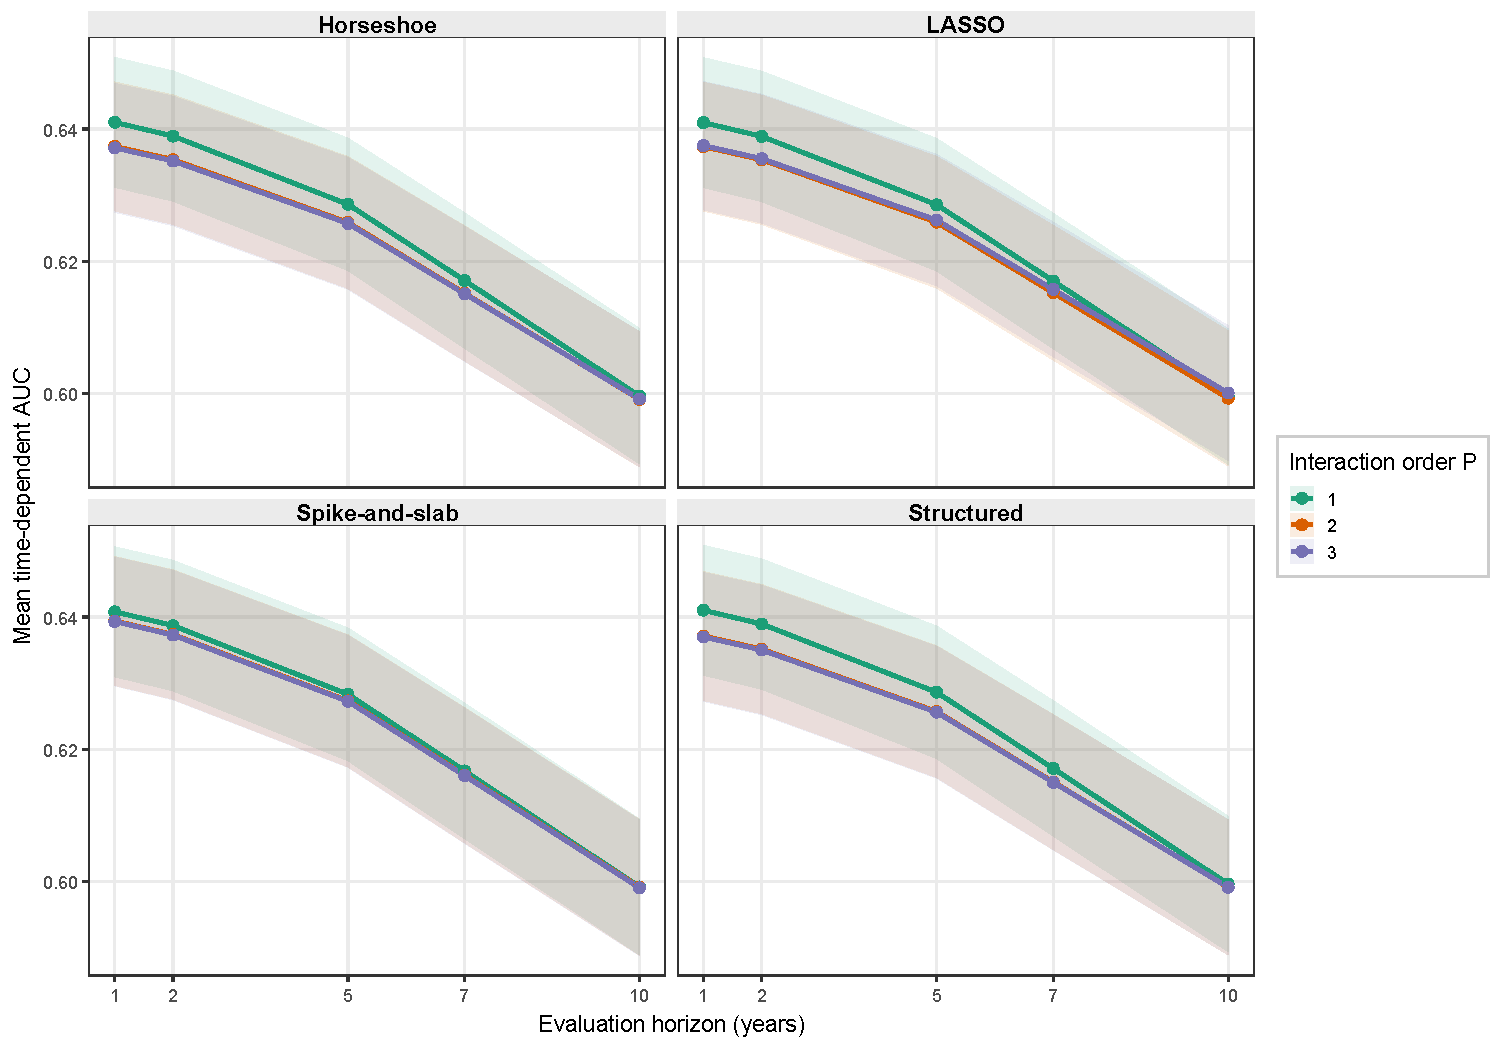
\includegraphics[width=\linewidth]{figures/fig_521a_order_tdauc}
\caption{Time-dependent AUC by interaction order $P \in \{1,2,3\}$ across all
prior families. Evaluation horizons $\tau \in \{1, 2, 5, 7, 10\}$ years are shown as labelled tick marks on the x-axis. Ribbons: $\pm1.96$\,SE across folds.}
\label{fig:order_tdauc}
\end{figure}

\begin{figure}[H]
\centering
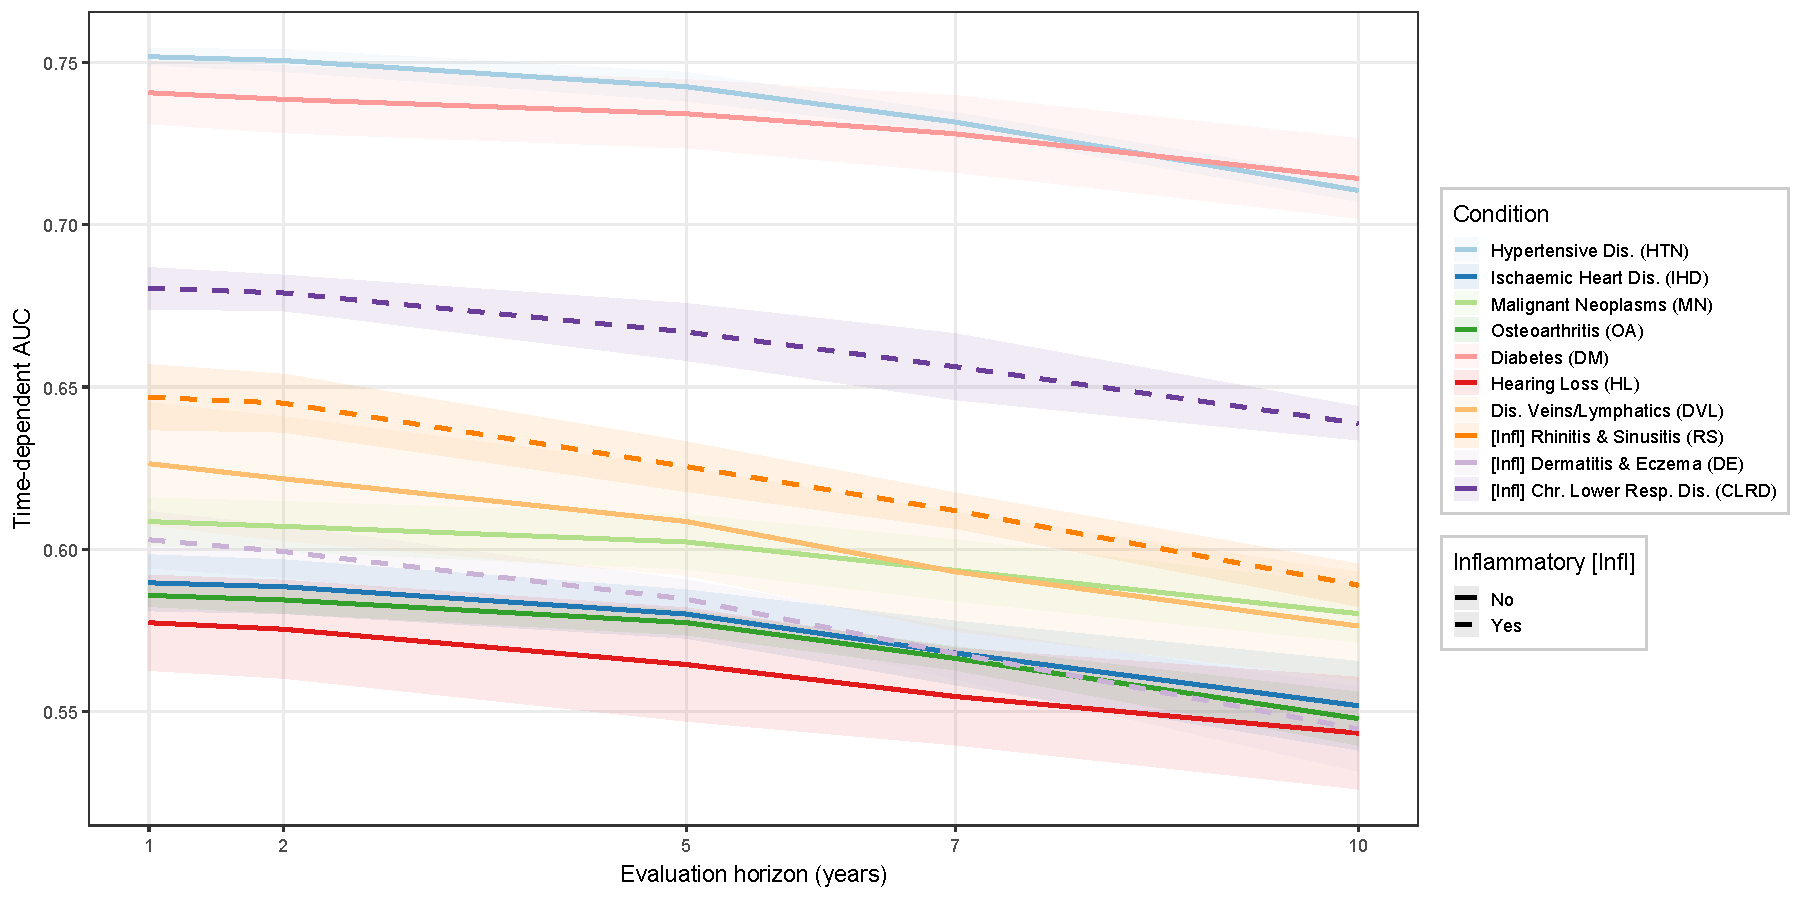
\includegraphics[width=\linewidth]{figures/fig_523_best_model_profile}
\caption{Per-condition tdAUC for the recommended model (spike-and-slab,
$P=2$, $\theta=1$).  \textbf{Dashed lines} = inflammatory conditions.
Ribbons: $\pm1.96$\,SE across folds.}
\label{fig:best_model_profile}
\end{figure}

\subsection{Inferred Multimorbidity Network}
\label{sec:network}

Figure~\ref{fig:pip_heatmap} displays the $10 \times 10$ posterior inclusion probability (PIP) heatmap of directed condition-to-condition edges. The strongest directed edges within the cardiometabolic cluster are $\text{DM} \to \text{HTN}$ ($\text{PIP} = 1.00$), 
$\text{DM} \to \text{IHD}$ ($\text{PIP} = 0.96$), and $\text{HTN} \to \text{IHD}$ ($\text{PIP} = 1.00$), confirming a dense and well-supported interdependence among these conditions. IHD further influences DM ($\text{PIP} = 1.00$) and HL ($\text{PIP} = 0.98$), 
and $\text{HL} \to \text{IHD}$ achieves $\text{PIP} = 1.00$, suggesting bidirectional reinforcement within this cluster. Within the inflammatory cluster, 
$\text{RS} \to \text{DE}$ ($\text{PIP} = 1.00$), $\text{RS} \to \text{CLRD}$ ($\text{PIP} = 1.00$), $\text{CLRD} \to \text{RS}$ ($\text{PIP} = 1.00$), and 
$\text{CLRD} \to \text{DE}$ ($\text{PIP} = 0.99$) all achieve near-certain inclusion, consistent with shared atopic and airway-inflammation mechanisms. Cross-cluster edges are notably sparser; $\text{MN} \to \text{DVL}$ ($\text{PIP} = 1.00$), $\text{IHD} \to \text{HL}$ ($\text{PIP} = 0.98$), $\text{OA} \to \text{RS}$ ($\text{PIP} = 0.92$), and $\text{OA} \to \text{DE}$ ($\text{PIP} = 0.96$) represent the most robust inter-cluster links, while $\text{HTN} \to \text{OA}$ ($\text{PIP} = 0.52$) and $\text{HL} \to \text{DE}$ ($\text{PIP} = 0.63$) suggest weaker but non-negligible associations.

Figure~\ref{figA:rr_network} presents the corresponding posterior mean rate ratios for all active edges, where the posterior mean rate ratio for edge $j \to m$ is defined as $\widehat{\text{RR}}_j^m = \exp(\hat{\beta}^m_{\{j\}})$ with $\hat{\beta}^m_{\{j\}} = \mathbb{E}[\beta^m_{\{j\}} \mid \mathcal{D}]$. The largest estimated effects are $\text{DM} \to \text{HTN}$ ($\widehat{\text{RR}} = 2.13$) and $\text{HTN} \to \text{DM}$ ($\widehat{\text{RR}} = 2.61$), indicating a strongly mutually reinforcing cardiometabolic relationship. Within the inflammatory cluster, $\text{CLRD} \to \text{RS}$ ($\widehat{\text{RR}} = 2.09$) and $\text{RS} \to \text{DE}$ ($\widehat{\text{RR}} = 1.95$) represent the largest inflammatory cross-effects. 
$\text{HTN} \to \text{IHD}$ ($\widehat{\text{RR}} = 1.67$) and $\text{IHD} \to \text{DM}$ ($\widehat{\text{RR}} = 2.01$) further highlight the magnitude of cardiometabolic cascading. All active edges are excitatory ($\widehat{\text{RR}} > 1$), 
indicating that the presence of any active influencer condition uniformly accelerates the onset of its target condition.

Figure~\ref{fig:network_graph} represents the network as a directed graph annotated with per-edge transition rates (per 1{,}000 person-years). Two distinct modules are visible: a dense cardiometabolic cluster comprising HTN, IHD, DM, and HL, and an inflammatory cluster comprising RS, DE, and CLRD, with OA, MN, and DVL occupying more peripheral roles. The 
highest transition rates are observed for $\text{DM} \to \text{HTN}$ ($57.6~\text{per}~1{,}000$) and $\text{HTN} \to \text{IHD}$ 
($35.4~\text{per}~1{,}000$), reflecting the high progression burden within the cardiometabolic pathway. Cross-cluster connectivity is primarily driven by OA linking to the inflammatory conditions and MN connecting to HL. Full active edge details are provided in Appendix Table~\ref{tab:network_edges}.

\begin{figure}[H]
\centering
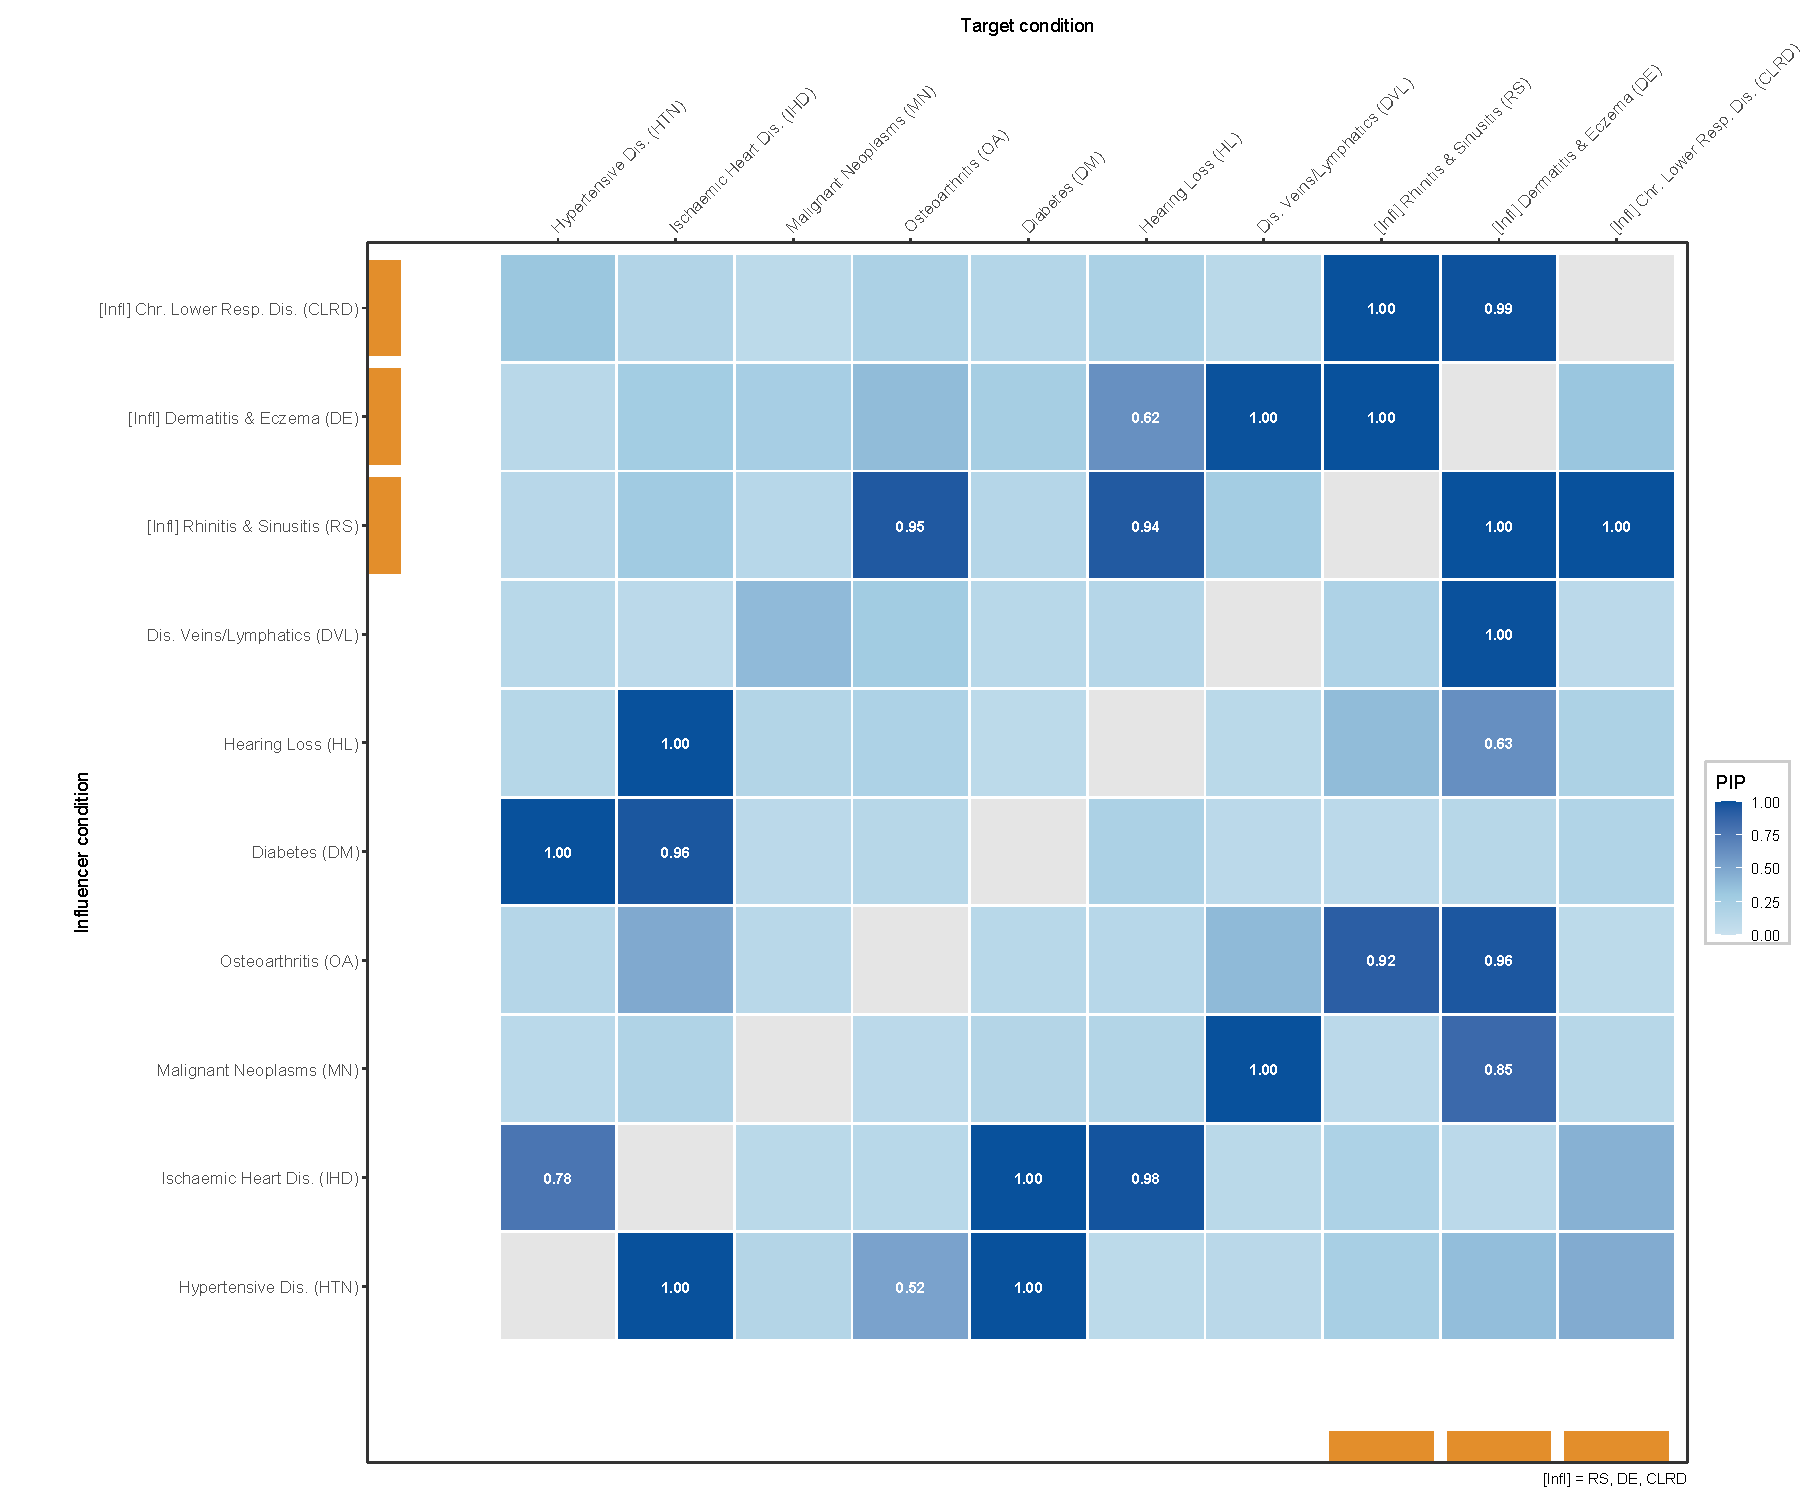
\includegraphics[width=\linewidth]{figures/fig_524a_pip_heatmap}
\caption{Posterior inclusion probability matrix.  Rows = influencer; columns = target.  Bold white text: active edges (PIP\,$\geq$\,0.50).  \textbf{Amber bar} = inflammatory cluster ([Infl]\,RS, [Infl]\,DE, [Infl]\,CLRD).  Spike-and-slab;
$\theta=1$; $P=2$.} \label{fig:pip_heatmap}
\end{figure}



\begin{figure}[H]
\centering
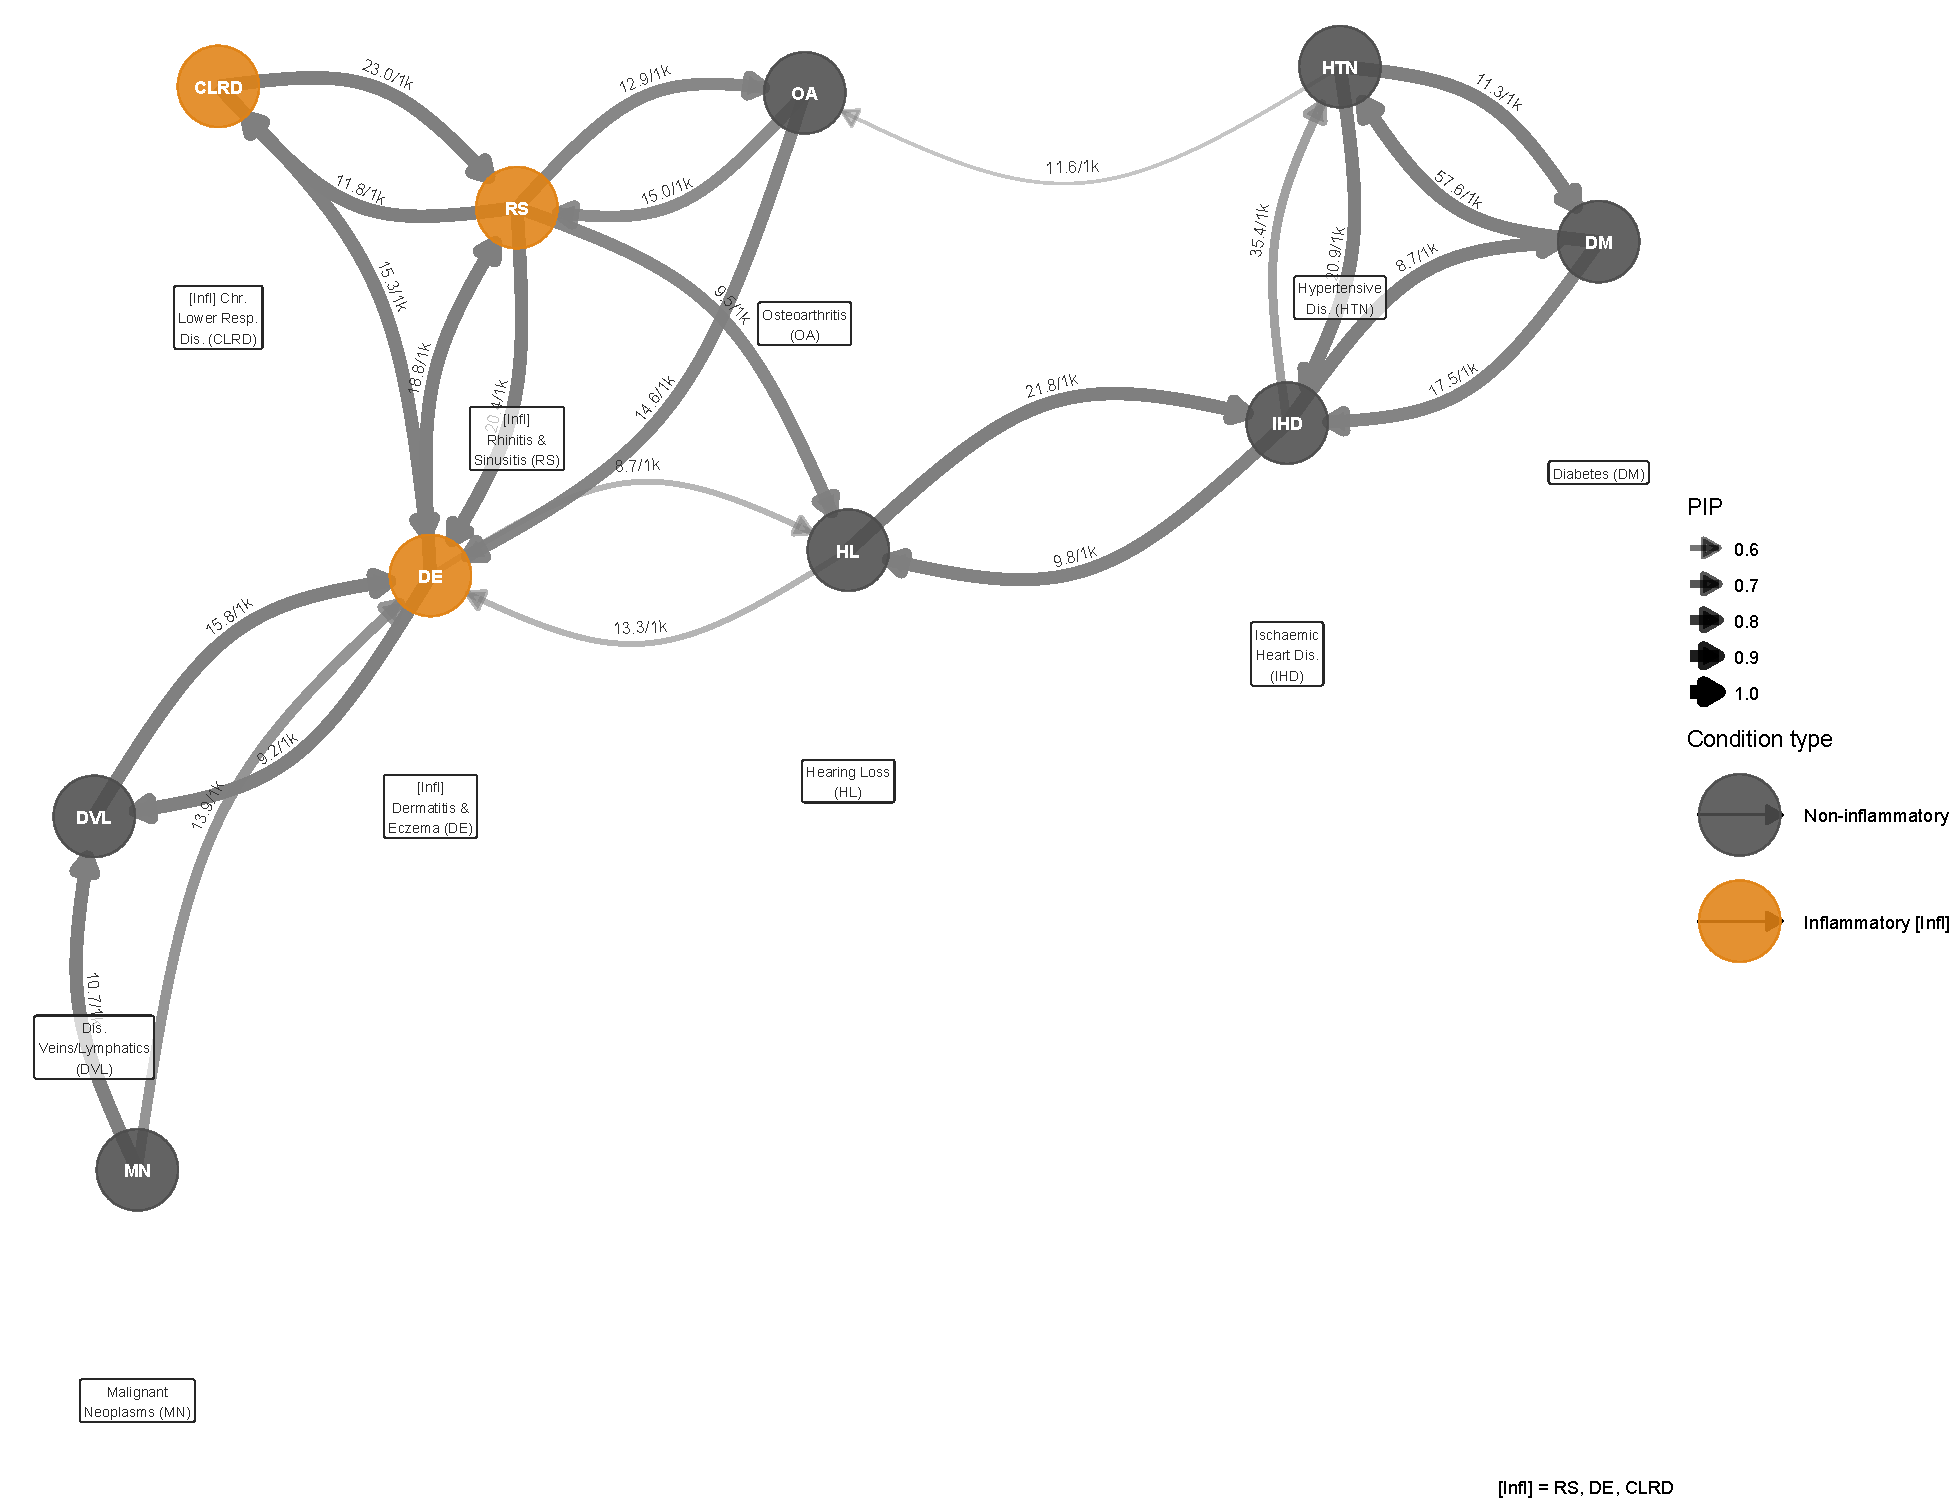
\includegraphics[width=0.95\linewidth]{figures/fig_524c_network_graph}
\caption{Directed multimorbidity network (PIP\,$\geq$\,0.50).  \textbf{Orange nodes} = inflammatory conditions.  Edge width $\propto$ PIP; labels = conditional intensity (events/1,000\,py).}
\label{fig:network_graph}
\end{figure}

\subsection{Conditional Risk of a Second Long-Term Condition}
\label{sec:conditional_risk}

Figure~\ref{fig:excess_risk} maps the 5-year excess cumulative incidence $\Delta^{(1)}_m(j) = F_m(5 \mid X_j = 1) - F_m(5 \mid X_j = 0)$ for all 90 off-diagonal condition pairs, evaluated at population-mean covariate values. The largest excess risk arises within the cardiometabolic cluster: individuals with 
existing DM face a $+12.4$ percentage point (pp) excess risk of developing HTN (conditional risk $25.0\%$ vs.\ baseline $12.6\%$; $\widehat{\text{RR}} = 2.13$), representing the single most clinically consequential directed association in the network. Other notable cardiometabolic pairs include $\text{HTN} \to \text{IHD}$ ($+3.8$\,pp; $\widehat{\text{RR}} = 1.67$), $\text{HL} \to \text{IHD}$ ($+4.2$\,pp; $\widehat{\text{RR}} = 1.74$), and $\text{HTN} \to \text{DM}$ ($+3.4$\,pp; $\widehat{\text{RR}} = 2.61$), the latter notable for its large relative effect despite a lower baseline incidence of DM ($2.1\%$).

Within the inflammatory cluster, $\text{CLRD} \to \text{RS}$ ($+5.5$\,pp; $\widehat{\text{RR}} = 2.09$) and $\text{RS} \to \text{DE}$ ($+4.6$\,pp; 
$\widehat{\text{RR}} = 1.95$) confirm that chronic airway disease substantially elevates the onset of upper respiratory and atopic conditions, consistent with shared mucosal inflammatory pathways. $\text{DE} \to \text{RS}$ also contributes a non-trivial excess risk ($+3.6$\,pp; $\widehat{\text{RR}} = 1.70$), indicating bidirectional reinforcement within the atopic triad. A modest but notable cross-cluster association is observed for $\text{MN} \to \text{DVL}$ ($+2.2$\,pp; $\widehat{\text{RR}} = 1.74$), plausibly reflecting treatment-related vascular sequelae. Several entries yield near-zero or marginally negative excess risks, most prominently $\text{DVL} \to \text{HTN}$ ($-0.9$\,pp), suggesting that DVL 
confers negligible additional risk for HTN beyond shared background factors. The top 15 condition pairs by excess absolute risk are provided in Appendix Table~\ref{tab:conditional_risk}.

\begin{figure}[H]
\centering
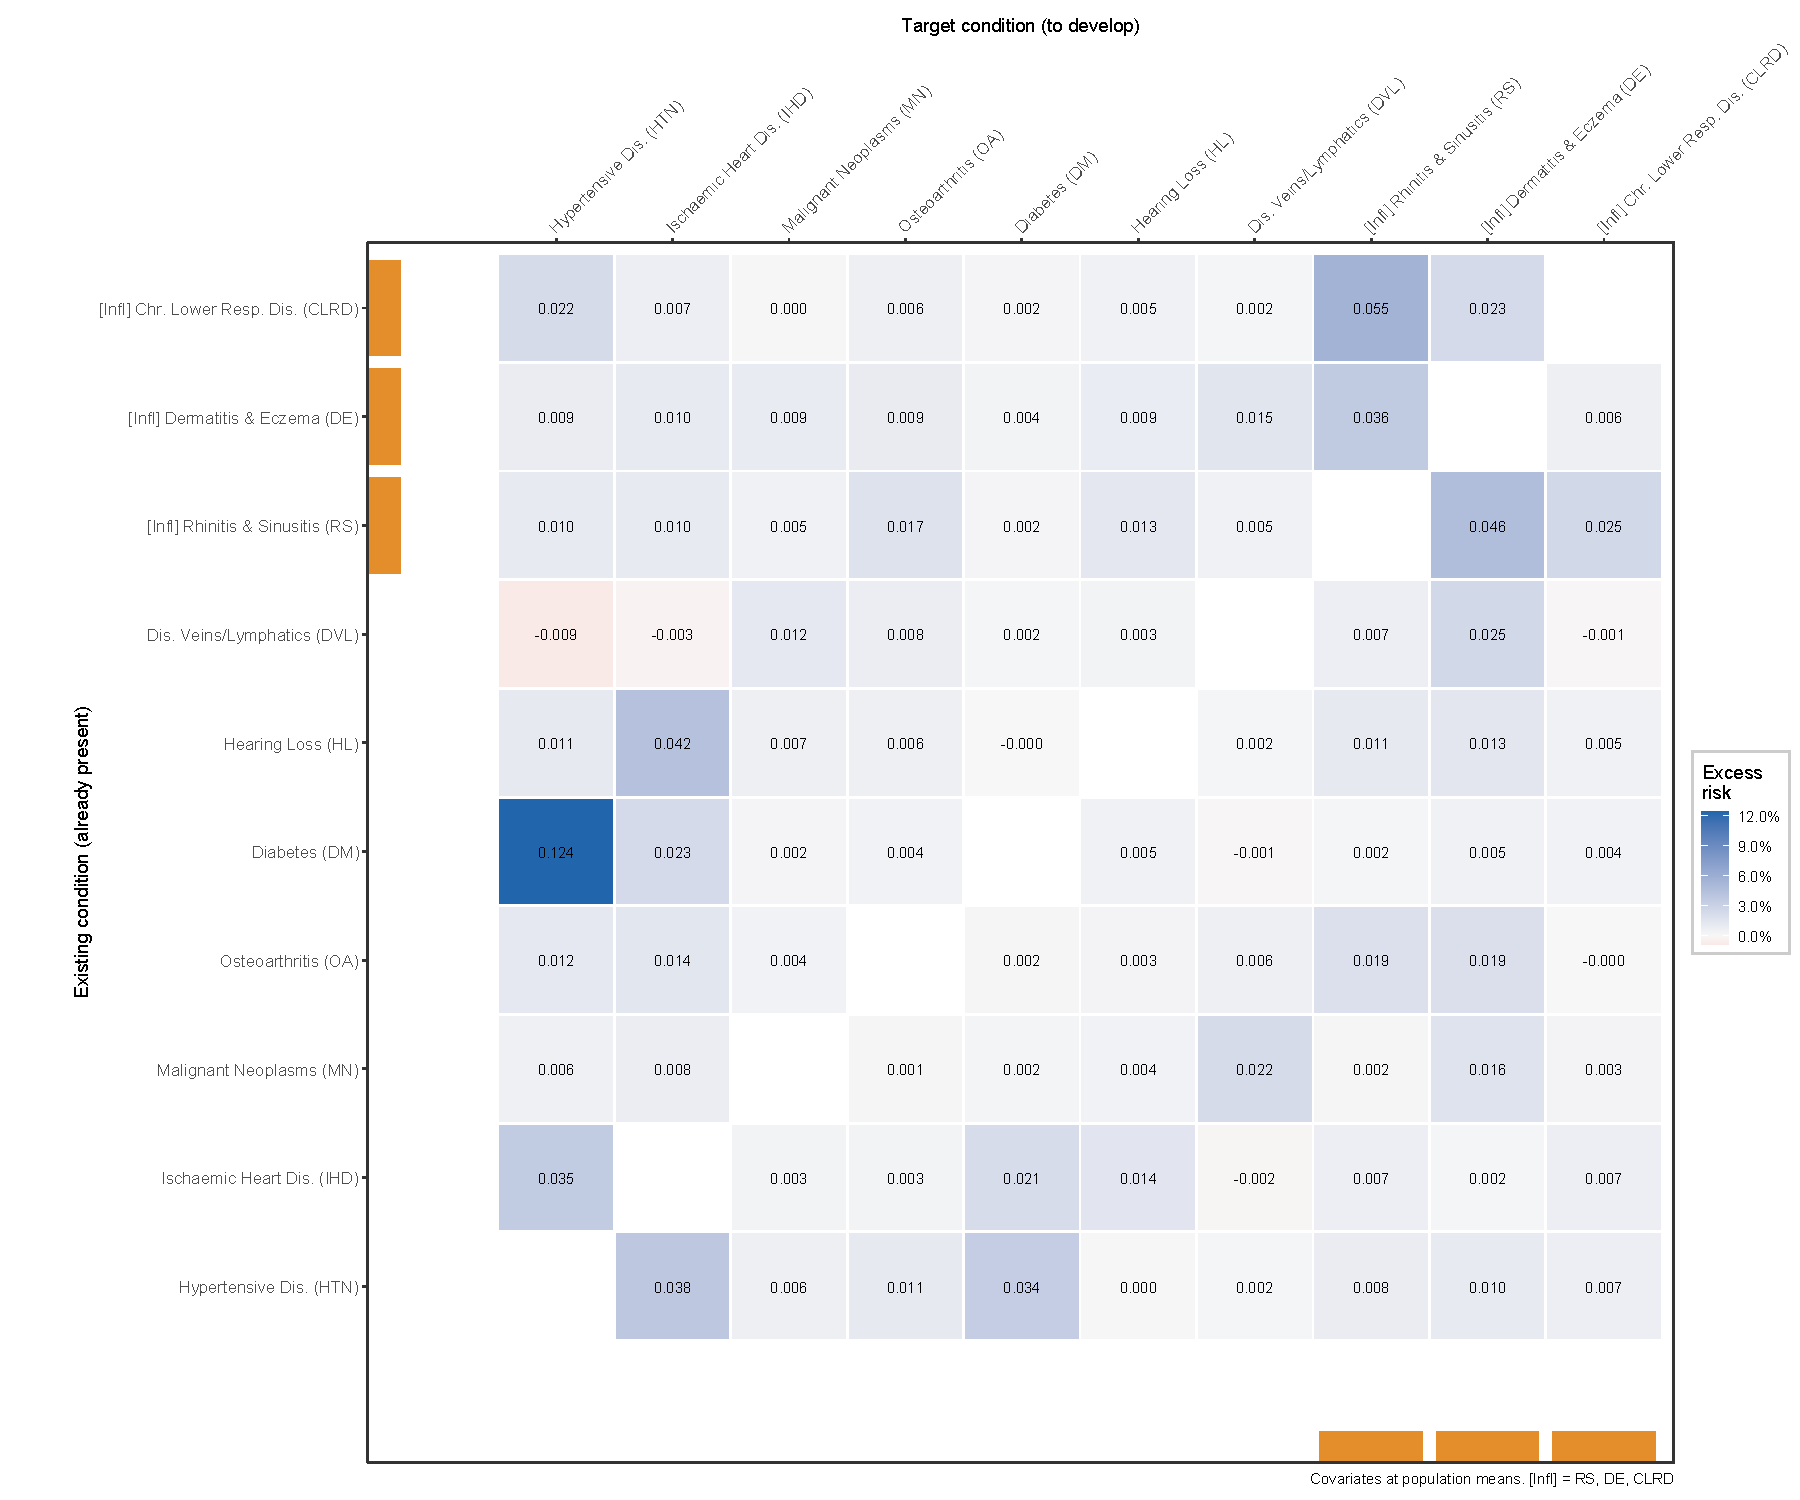
\includegraphics[width=\linewidth]{figures/fig_525a_excess_risk_heatmap}
\caption{Five-year excess cumulative incidence
$\Delta^{(1)}_m(j) = F_m(5 \mid X_j=1,\,\mathbf{Z}=\bar{\mathbf{Z}}) -
F_m(5 \mid X_j=0,\,\mathbf{Z}=\bar{\mathbf{Z}})$.
Blue = increased risk; red = reduced risk.
\textbf{Amber bar} = inflammatory cluster; diagonal suppressed.}
\label{fig:excess_risk}
\end{figure}

\subsubsection{Synergistic Risk of a Third Long-Term Condition}
\label{sec:interaction_effects}

For a patient with two conditions $j$ and $k$ simultaneously present, the onset 
rate for a third condition $m$ decomposes as:
\[
q_m(j,k)
= \underbrace{\exp(\beta^0_m + \bar{\mathbf{Z}}^\top\boldsymbol{\gamma}_m)}_{\text{baseline}}
\times
\underbrace{e^{\beta^m_{\{j\}}}}_{\mathrm{RR}_j}
\times
\underbrace{e^{\beta^m_{\{k\}}}}_{\mathrm{RR}_k}
\times
\underbrace{e^{\beta^m_{\{j,k\}}}}_{\text{synergistic multiplier}}.
\]
The synergistic multiplier $e^{\beta^m_{\{j,k\}}}$ is the exponentiated two-way interaction coefficient of equation~\eqref{eqn1}: a value $> 1$ indicates super-multiplicative synergy and a value $< 1$ sub-multiplicative antagonism. Active interactions are declared at $\text{PIP}_{jk}^{m} \geq 0.50$.

On the cumulative incidence scale we define the \emph{synergistic excess} at horizon $\tau$ as
\begin{equation}\label{eq:synergy_excess}
\Delta F_m(\tau)
= \underbrace{F_m(\tau \mid X_j=1, X_k=1)}_{\text{joint exposure}}
-\;
\underbrace{\bigl[F_m(\tau \mid X_j=1, X_k=0) + F_m(\tau \mid X_j=0, X_k=1) - F_m(\tau \mid X_j=0, X_k=0)\bigr]}_{\text{additive counterfactual}},
\end{equation}
evaluated at population-mean covariate values $\bar{\mathbf{Z}}$. The bracketed term is the cumulative incidence that would arise if the two conditions acted purely additively on the cumulative incidence scale (so $\Delta F_m(\tau)$ equals zero in the absence of a two-way interaction in the log-rate); $\Delta F_m(\tau)$ therefore translates the interaction coefficient $\beta^m_{\{j,k\}}$ into clinically interpretable percentage-point units. Positive $\Delta F_m(\tau)$ indicates super-multiplicative excess (joint exposure yields more cumulative risk than the sum of marginal exposures), negative $\Delta F_m(\tau)$ indicates sub-multiplicative attenuation.

Four triplets achieve high posterior inclusion ($\text{PIP}_{jk}^{m} \geq 0.997$), all exhibiting sub-multiplicative antagonism (synergistic multiplier $< 1$), and are summarised in Appendix Table~\ref{tab:interaction_decomp}. The triplet $\{\text{RS},\,\text{DM}\} \to \text{HTN}$ yields the largest synergistic excess in absolute terms ($\Delta F_m(5) = \pm7.7$\,pp; synergistic multiplier $= 0.646$; joint $\widehat{\text{RR}} = 1.491$), indicating that despite the large individual effects of RS ($\widehat{\text{RR}}_j = 1.084$) and DM 
($\widehat{\text{RR}}_k = 2.129$), their co-occurrence attenuates the expected multiplicative hazard on HTN onset. Similarly, $\{\text{IHD},\,\text{DM}\} \to 
\text{HTN}$ produces a $\pm7.4$\,pp synergistic excess (synergistic multiplier $= 0.631$; joint $\widehat{\text{RR}} = 1.755$), while 
$\{\text{HTN},\,\text{DM}\} \to \text{IHD}$ yields $\pm3.3$\,pp (synergistic multiplier $= 0.642$; joint $\widehat{\text{RR}} = 1.498$). The $\{\text{HTN},\,\text{IHD}\} \to \text{DM}$ triplet, despite having the largest individual rate ratios ($\widehat{\text{RR}}_j = 2.610$, $\widehat{\text{RR}}_k = 2.011$), exhibits the strongest attenuation (synergistic multiplier $= 0.591$; joint $\widehat{\text{RR}} = 3.099$), resulting in the smallest synergistic excess ($\pm1.1$\,pp), suggesting a ceiling effect in 
which already-elevated individual risks leave limited room for further multiplicative amplification.

Figure~\ref{fig:synergy_forest} presents the synergistic excess risk $\Delta F_m(5)$ for the four triplets by absolute magnitude, confirming that 
sub-multiplicative interactions predominate across all four high-PIP triplets and that the largest effects are concentrated within the cardiometabolic cluster. 
Figure~\ref{fig:synergy_curves} displays the cumulative incidence trajectories $F_m(t)$ over 10 years for these four triplets. In all panels, the trajectory for both conditions present lies below the multiplicative combination of the two individual-condition trajectories, visually confirming sub-multiplicative antagonism. The gap between the joint trajectory and the baseline (neither condition present) nonetheless remains substantial, most prominently for $\{\text{IHD},\,\text{DM}\} \to \text{HTN}$, where cumulative incidence under joint exposure approaches $50\%$ by year 10. Full decomposition details are provided in Appendix 
Table~\ref{tab:interaction_decomp}.

\begin{figure}[H]
\centering
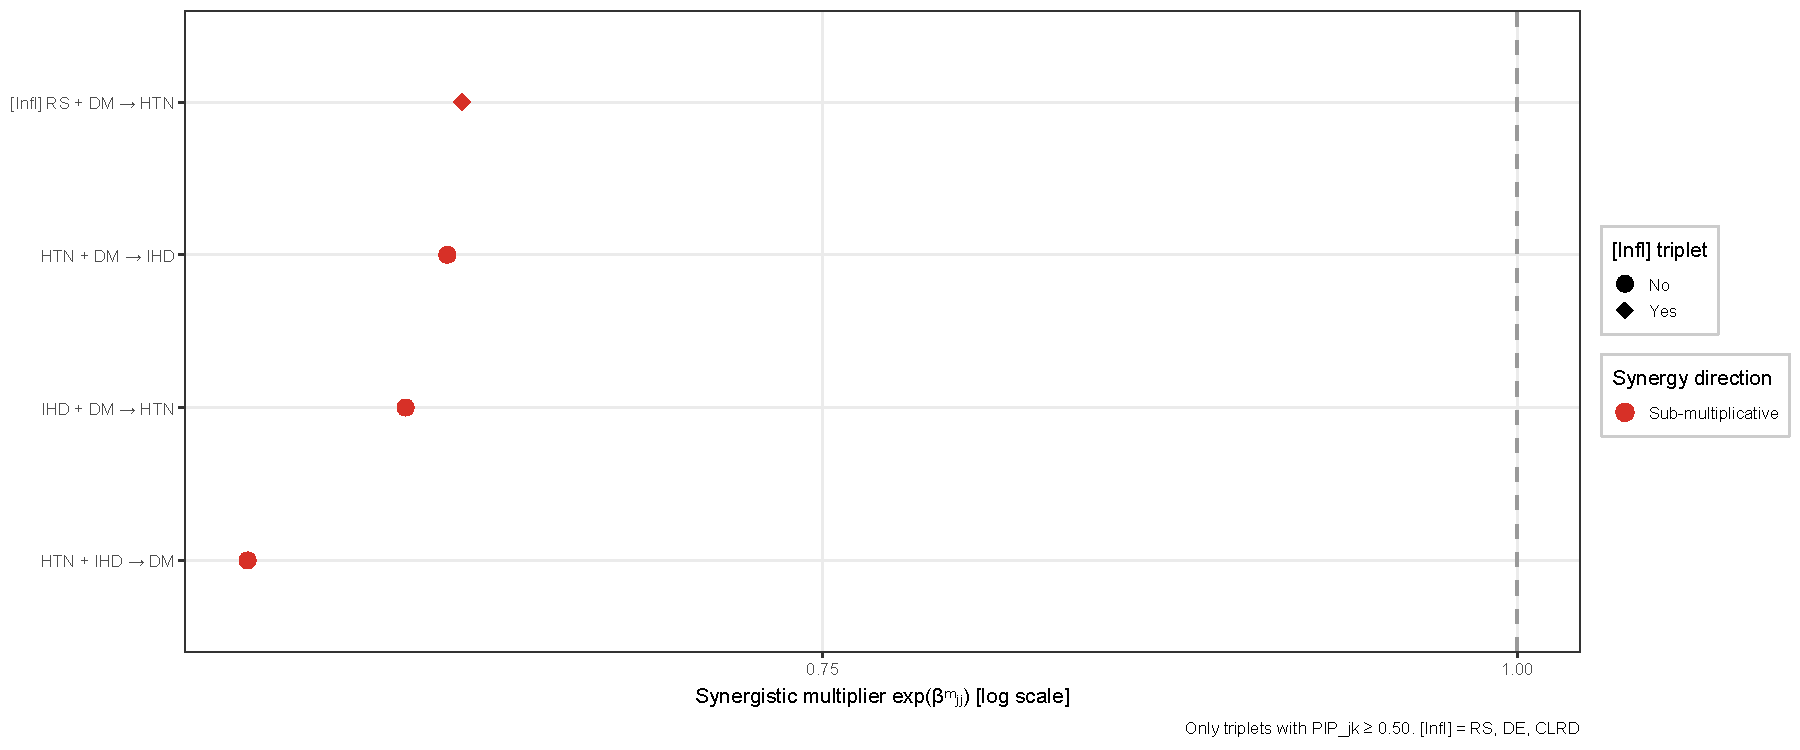
\includegraphics[width=\linewidth]{figures/fig_526a_synergy_forest}
\caption{Synergistic multiplier $\exp(\hat{\beta}^m_{\{j,k\}})$ for all
significant triplets (PIP$_{jk} \geq 0.50$).  Blue $>$\,1 = super-multiplicative;
red $<$\,1 = sub-multiplicative.  $\blacklozenge$ = triplet involving
inflammatory cluster.}
\label{fig:synergy_forest}
\end{figure}

\begin{figure}[H]
\centering
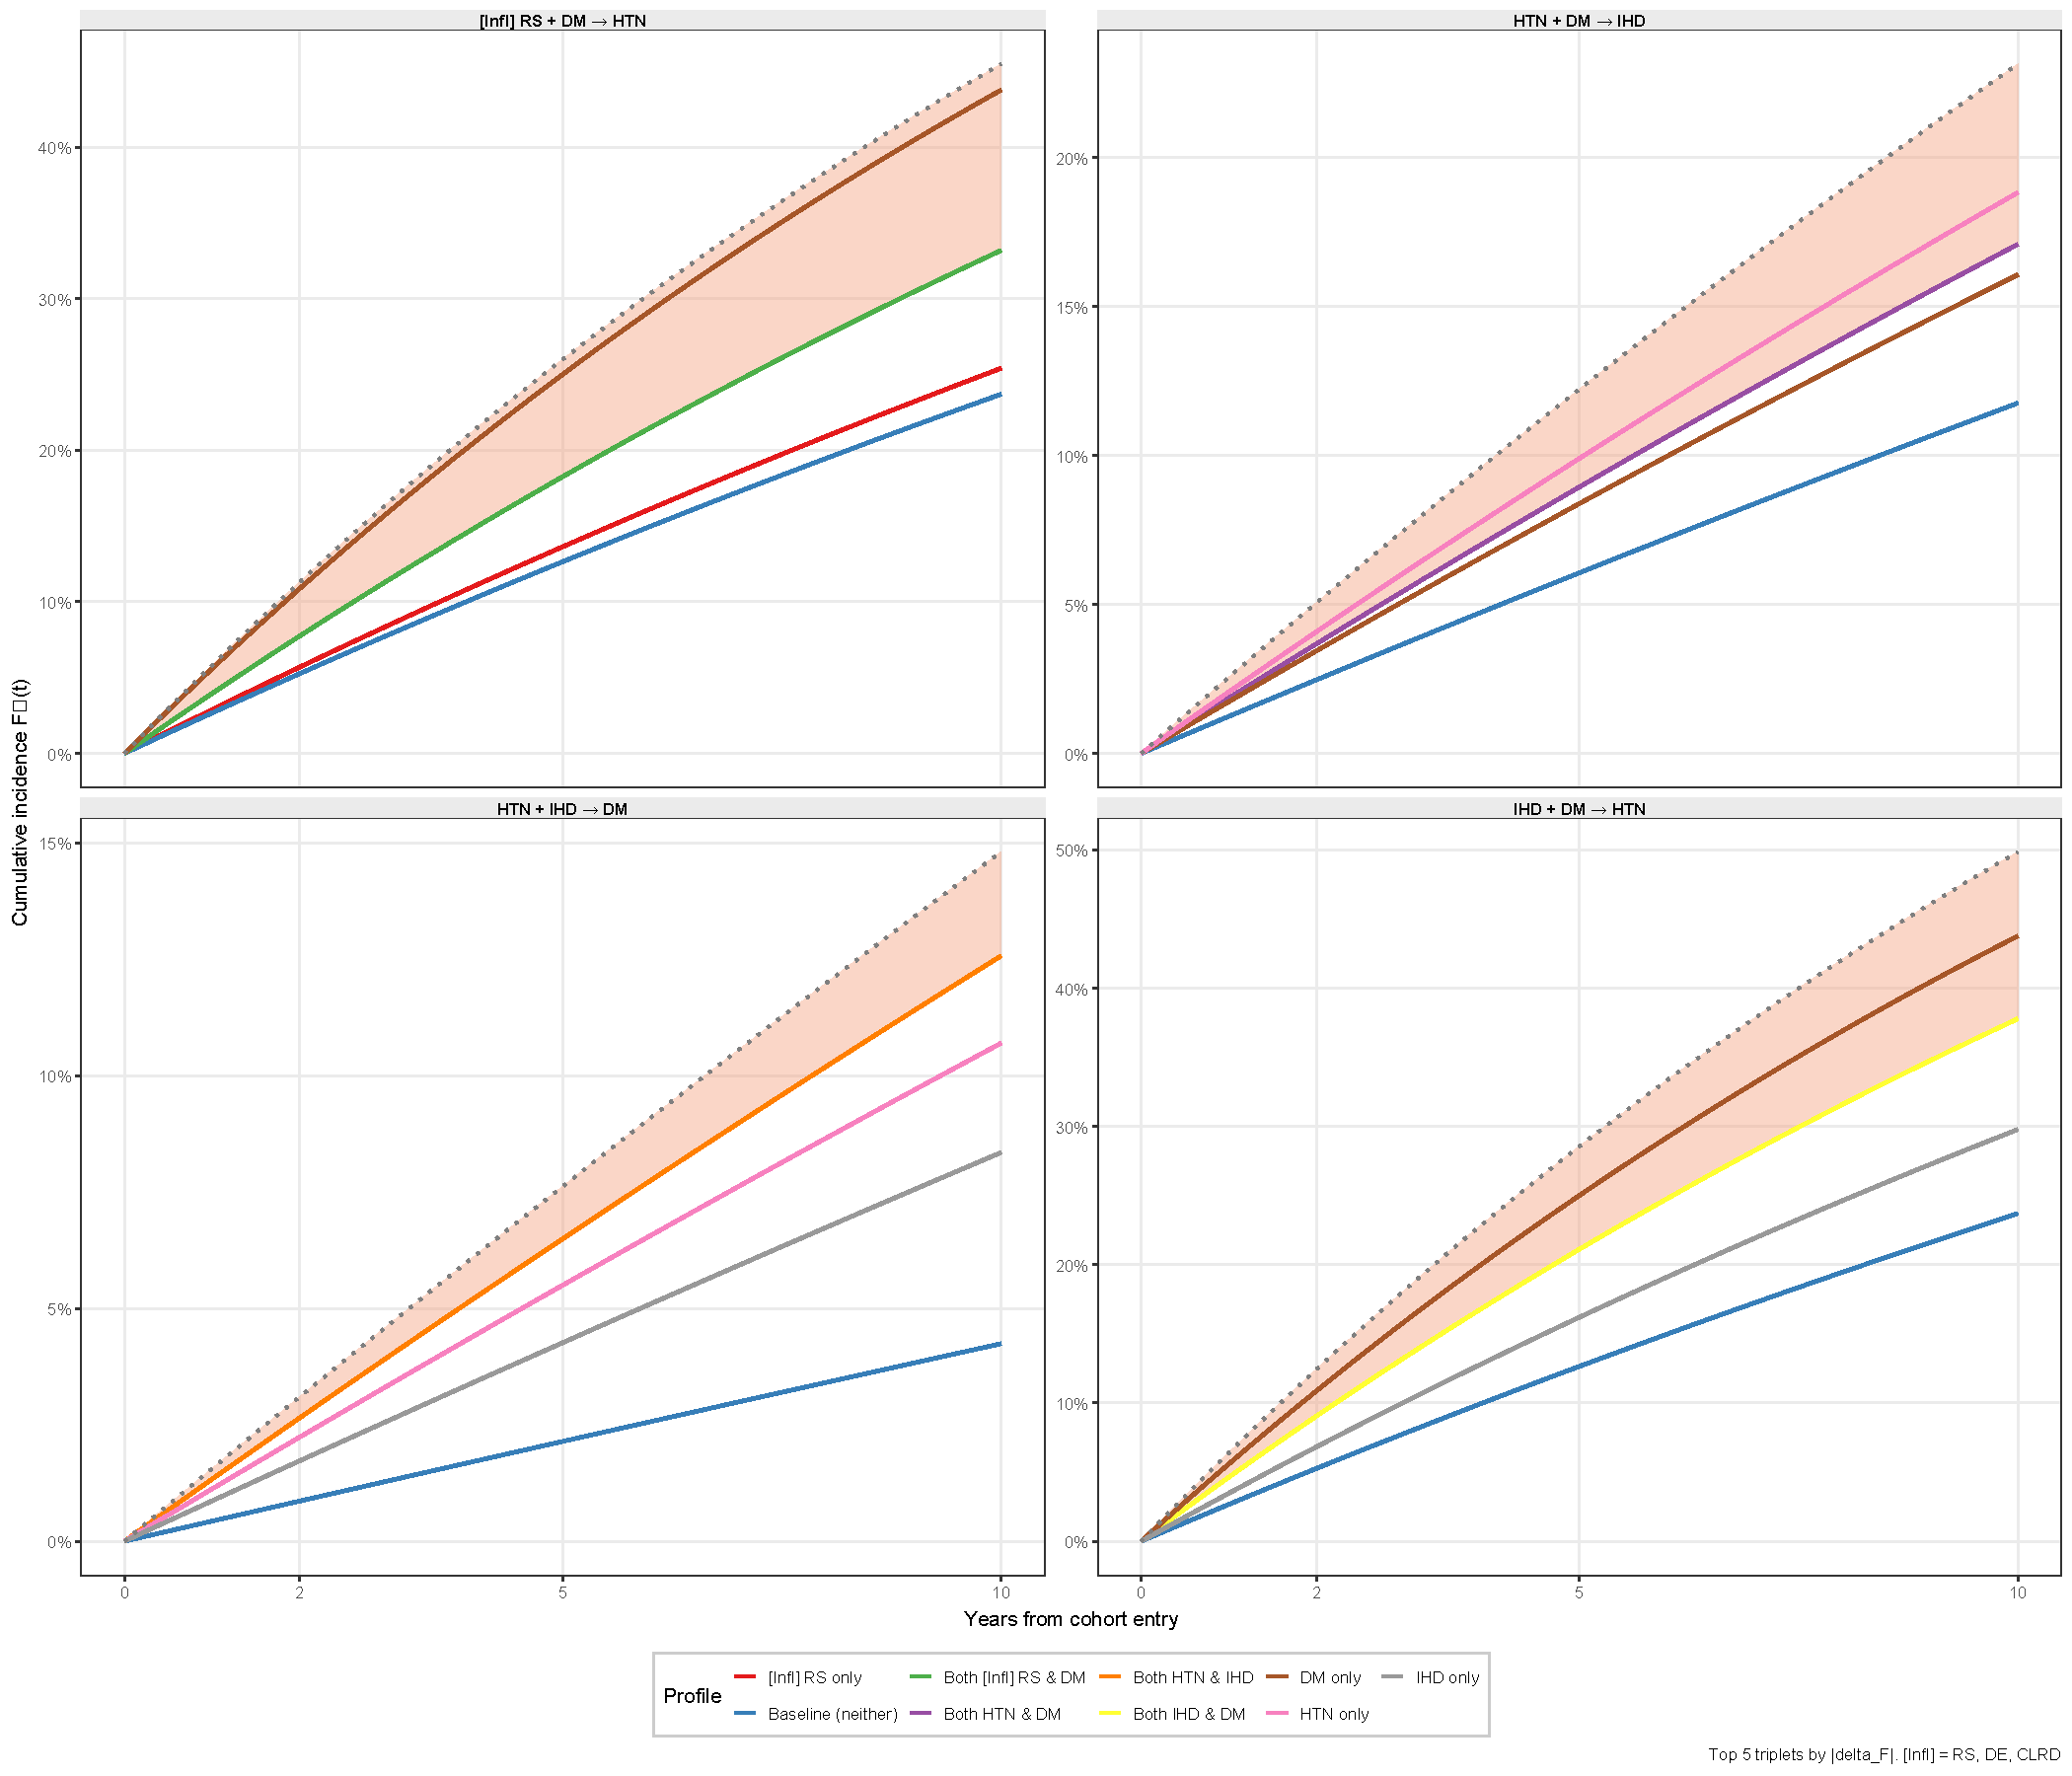
\includegraphics[width=\linewidth]{figures/fig_526c_synergy_curves}
\caption{Cumulative incidence $\hat{F}_m(t)$ under four disease profiles for
the four triplets with the largest significant $|\Delta F_m(5)|$.  Orange ribbon = synergistic excess (joint\,$-$\,additive counterfactual).  Dotted line =
additive counterfactual.  Covariates at population means.} \label{fig:synergy_curves}
\end{figure}

\subsection{Covariate Associations}
\label{sec:covariates_results}

Figure~\ref{fig:pip_covariates} shows that age achieves PIP\,=\,1.00 across all conditions, confirming it as the strongest and most consistent predictor of chronic disease onset. This is consistent with the well-established age-dependence of all ten conditions modelled here, whose incidence rises sharply across the adult age range in primary-care populations.  Among fixed biomarkers, WBC, Platelet, GlycA, Neutrophil, Lymphocyte, and WBC achieve the highest PIPs for cardiometabolic targets, consistent with evidence from the wider EHR literature linking systemic inflammatory biomarkers to CVD risk. Current and former smoking attain PIP\,$\geq$\,0.50 for [Infl]\,CLRD, consistent with the established role of tobacco exposure in airway
inflammation.  BMI\,$>$\,30 is selected for HTN, MN, OA, DM, and HL, reflecting the obesity-related conditions. Also, Sex is associated with IHD, OA, DM, HL, [Infl]\,RS and [Infl]\,CLRD.

\begin{figure}[H]
\centering
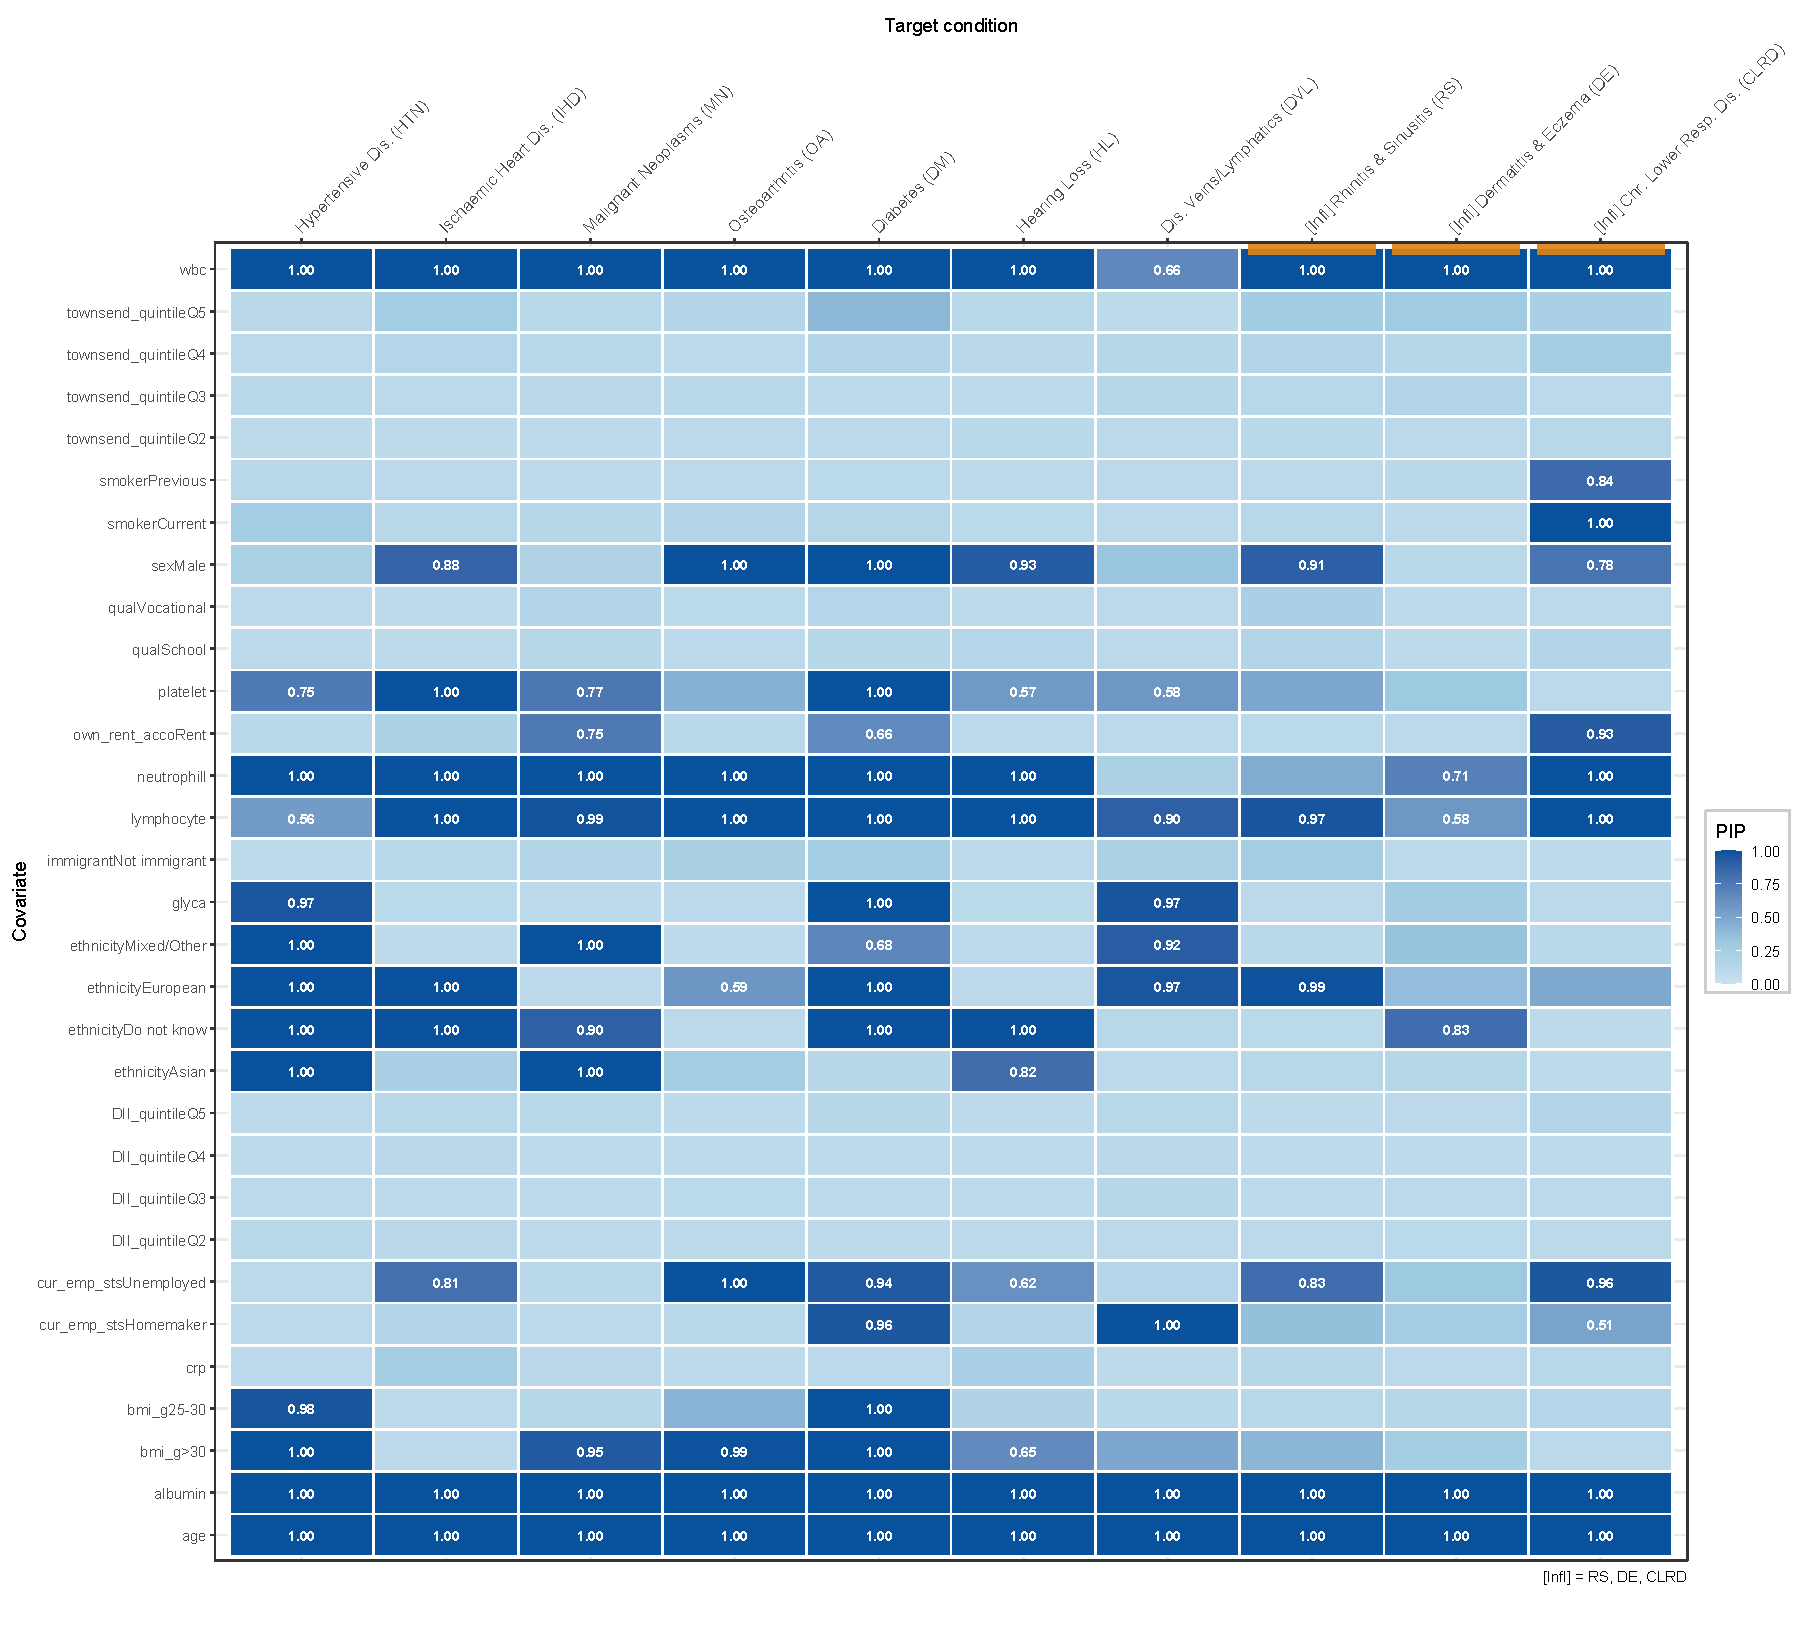
\includegraphics[width=\linewidth]{figures/fig_529a_pip_covariates}
\caption{Posterior inclusion probabilities for covariate effects.  Bold white
text: PIP\,$\geq$\,0.50.  Amber bar = inflammatory target columns.
Spike-and-slab; $\theta=1$; $P=2$.}
\label{fig:pip_covariates}
\end{figure}

Posterior mean rate ratios (Figure~\ref{fig:rr_covariates_forest}) confirm clinically expected directions across excitatory covariates. Older age is the most pervasive risk factor, elevating onset rates across all ten conditions. Male sex is associated with higher onset rates for IHD, DM, HL, and CLRD. Current and previous smoking substantially elevate the onset rate for CLRD, consistent with its established aetiology. Elevated GlycA accelerates cardiometabolic onset, particularly for HTN and DM, while higher BMI ($>$30) is associated with increased onset rates for HTN, DM, and OA. Among haematological markers, elevated neutrophil and lymphocyte counts are broadly associated with higher onset rates across cardiometabolic, inflammatory, and neoplastic conditions, with WBC additionally contributing to CLRD onset. Socioeconomic indicators such as unemployment and renting also emerge as risk-elevating covariates across several conditions including IHD, OA, DM, HL and RS.
Conversely, Figure~\ref{fig:rr_covariates_forest2} reveals a distinct set of inhibitory covariates associated with reduced onset rates (RR\,$\ll$\,1). Albumin is the most consistent protective factor, with lower onset rates observed across all ten conditions, reflecting its role as a marker of nutritional status and systemic health. Platelet count and WBC are also associated with reduced onset rates for several conditions including DM, IHD, MN, and DVL. Ethnicity-related heterogeneity is also evident, with Asian and European ethnicities showing condition-specific reductions relative to the African reference group. The full covariate rate ratio heatmap is provided in Appendix Figure~\ref{figA:rr_covariates}.

\begin{figure}[H]
\centering
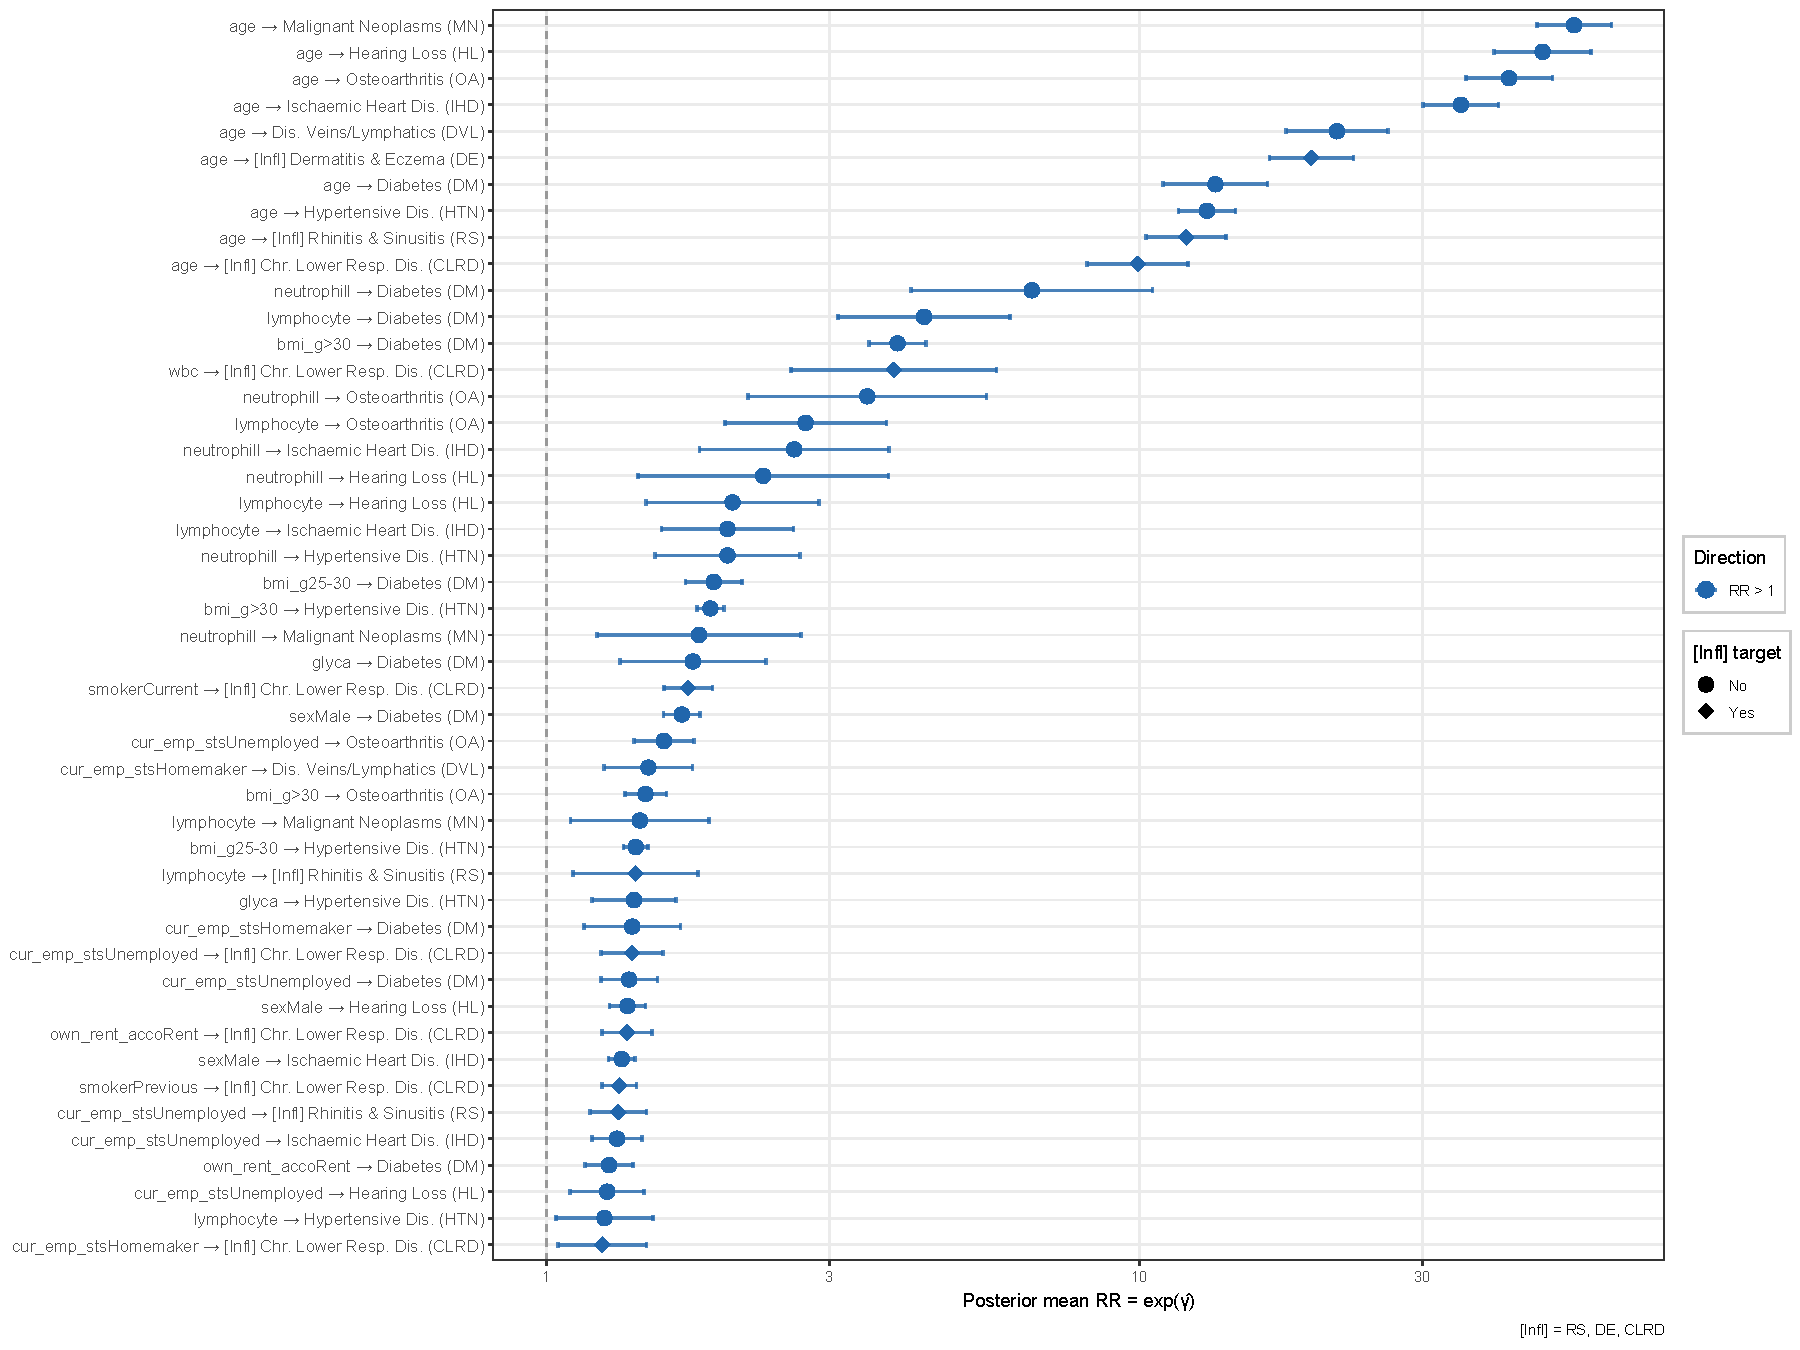
\includegraphics[width=\linewidth]{figures/fig_529c_covariate_forest}
\caption{Forest plot of posterior mean rate ratios for excitatory covariates (RR $>1$ and PIP\,$\geq$\,0.50).  95\% credible intervals from NUTS.
Spike-and-slab; $\theta=1$; $P=2$.}
\label{fig:rr_covariates_forest}
\end{figure}


\section{Simulation Study}\label{sec:sim}

To rigorously evaluate the performance of the CTBN framework with structured shrinkage priors, we conducted a simulation study designed to mirror the empirical data structure of the UK Biobank analysis while enabling ground truth comparisons. The simulation parameters were calibrated to estimates derived from the real-data analysis using the spike-and-slab prior, ensuring ecological validity under controlled conditions.

\subsection{Simulation Design and Network Structure}

The simulation network comprises ten binary conditions corresponding to those analysed in the empirical study: Malignant neoplasms (MN), Ischaemic heart diseases (IHD), Dermatitis and eczema (DE), Hypertensive diseases (HD), Diseases of veins and lymphatic vessels (DVL), Rhinitis and Sinusitis (RS), Conductive and sensorineural hearing loss (CSHL), Diabetes (Dia), Osteoarthritis (OA), and Chronic lower respiratory diseases (CLRD). Consistent with the notation of Section~3.1, each condition $X_m(t) \in \{0,1\}$ for $m = 1, \dots, 10$ evolves as a semi-absorbing continuous-time Markov process. Patient $i$, condition $m$, and time interval $s$ are indexed as throughout Sections~3.1--3.4.

The onset intensity for condition $m$ in interval $(i,s)$ follows the log-linear parameterisation of equation~\eqref{eqn1} with interactions up to order $P = 2$:
\[
\log q_{m,i,s} = \beta^0_m + \sum_{j \in \mathrm{Pa}(m)} \beta^m_{\{j\}}\, X_{j,i,s} + \sum_{\substack{L \subseteq \mathrm{Pa}(m) \\ |L| = 2}} \beta^m_L \prod_{j \in L} X_{j,i,s} + \mathbf{Z}_{i,s}^\top \boldsymbol{\gamma}_m,
\]
where $\beta^0_m$ is the baseline log-intensity, $\beta^m_{\{j\}}$ captures the main effect of parent condition $j$ on the onset of condition $m$, $\beta^m_L$ models the pairwise synergistic interaction between the two conditions in $L \subseteq \mathrm{Pa}(m)$, and $\boldsymbol{\gamma}_m$ encodes covariate effects. The absorbing-state intensity matrix for each condition is $Q_{m|u} = \bigl(\begin{smallmatrix} -q_{m,i,s} & q_{m,i,s} \\ 0 & 0 \end{smallmatrix}\bigr)$, reflecting the chronic nature of the conditions as established in Section~3.1.

The directed graph $\mathcal{G}$ was specified according to posterior inclusion probabilities exceeding 0.5 from the empirical spike-and-slab analysis, capturing the most robust probabilistic dependencies among conditions. The resulting structure includes Osteoarthritis and Rhinitis and Sinusitis as central nodes with multiple outgoing edges, a reciprocal relationship between Dermatitis and eczema and Rhinitis and Sinusitis, and Chronic lower respiratory diseases influenced by Rhinitis and Sinusitis alongside baseline covariates.

\subsection{Parameter Calibration from Empirical Estimates}

Parameter values were calibrated to align with empirical estimates from the spike-and-slab model. Baseline log-intensities $\beta^0_m$ were set to approximate observed one-year incidence rates from the UK Biobank, ranging from $\exp(\beta^0_m) = 0.005$ per year for Malignant neoplasms to $\exp(\beta^0_m) = 0.15$ per year for Hypertensive diseases. The interaction structure was sparse: approximately 80\% of possible pairwise coefficients $\beta^m_L$ were set to zero. The remaining 20\% received non-zero values drawn from a mixture: with probability 0.7, $\beta^m_L \sim \mathcal{N}(0, 0.3^2)$, representing weak to moderate synergistic effects, and with probability 0.3, $\beta^m_L \sim \mathcal{N}(0.8, 0.2^2)$, capturing stronger synergistic relationships consistent with known clinical comorbidity patterns.

The covariate vector $\mathbf{Z}_{i,s}$ for patient $i$ in interval $s$ contains three predictors. Age was modelled as a continuous time-varying covariate with initial distribution $\mathrm{age}_{i,0} \sim \mathcal{N}(57, 9.39^2)$ and deterministic progression $\mathrm{age}_{i,s} = \mathrm{age}_{i,0} + t_{i,s}$, where $t_{i,s}$ is the calendar time at the start of interval $s$. Sex was treated as a binary time-invariant covariate with $\Pr(\mathrm{male}) = 0.56$. Smoking status was treated as a time-varying categorical variable with three ordered states: never (0), former (1), and current (2) smoker. To respect the irreversibility of smoking cessation and the impossibility of reverting to never-smoker status, transitions are restricted to the one-directional process current $\to$ former and never $\to$ current, giving the intensity matrix
\[
Q_{\mathrm{smoking}} =
\begin{pmatrix}
-(q_{01}^{\mathrm{s}}) & q_{01}^{\mathrm{s}} & 0 \\
0 & -(q_{12}^{\mathrm{s}}) & q_{12}^{\mathrm{s}} \\
0 & 0 & 0
\end{pmatrix},
\]
where rows and columns correspond to never, former, and current smoking states respectively, $q_{01}^{\mathrm{s}} = 0.04$ is the rate of initiating smoking (never $\to$ current is not directly modelled; the path is never $\to$ former is not possible biologically; the states are never, current, former and only the transitions never $\to$ current and current $\to$ former are permitted), $q_{12}^{\mathrm{s}} = 0.06$ is the rate of cessation (current $\to$ former), and the absorbing state former reflects the permanent nature of having quit. The initial smoking distribution was set to $\mathrm{Categorical}(0.47, 0.11, 0.42)$ for never, current, and former respectively, calibrated to UK Biobank baseline prevalences. Covariate effects $\boldsymbol{\gamma}_m$ are reported in Table~\ref{tab:sim_cov_coeffs}, with age effects positive across all conditions and strongest for cardiovascular and metabolic diseases, and smoking effects most pronounced for respiratory and malignant conditions.

\begin{table}[H]
\footnotesize
\centering
\caption{True covariate coefficients ($\boldsymbol{\gamma}_m$) used in the simulation, calibrated to empirical estimates from the UK Biobank spike-and-slab analysis. Smoking effects are relative to the never-smoker reference category.}
\label{tab:sim_cov_coeffs}
\begin{tabular}{lcccc}
\hline
\textbf{Condition} & \textbf{Age} & \textbf{Sex (male)} & \textbf{Smoking (current)} & \textbf{Smoking (former)} \\
\hline
Malignant neoplasms (MN) & 0.25 & 0.15 & 0.35 & 0.10 \\
Ischaemic heart diseases (IHD) & 0.30 & 0.25 & 0.40 & 0.15 \\
Dermatitis and eczema (DE) & 0.05 & $-$0.10 & 0.10 & 0.05 \\
Hypertensive diseases (HD) & 0.35 & 0.20 & 0.25 & 0.10 \\
Diseases of veins/lymphatics (DVL) & 0.20 & 0.10 & 0.20 & 0.08 \\
Rhinitis and Sinusitis (RS) & 0.10 & 0.05 & 0.15 & 0.05 \\
Hearing loss (CSHL) & 0.40 & 0.30 & 0.20 & 0.10 \\
Diabetes (Dia) & 0.25 & 0.15 & 0.30 & 0.12 \\
Osteoarthritis (OA) & 0.45 & 0.10 & 0.15 & 0.05 \\
Chronic lower respiratory diseases (CLRD) & 0.30 & 0.20 & 0.60 & 0.20 \\
\hline
\end{tabular}
\end{table}

\subsection{Data Generation Mechanism}

We generated $N = 5{,}000$ independent patient trajectories over the time horizon $[0, 10]$ years. Initial condition states were drawn from Bernoulli distributions with prevalences calibrated to UK Biobank estimates: MN (0.06), IHD (0.08), DE (0.07), HD (0.16), DVL (0.04), RS (0.08), CSHL (0.04), Dia (0.05), OA (0.06), and CLRD (0.05). Initial covariate values were drawn from the distributions described in Section~4.2.

Patient trajectories were simulated using the following exact procedure, which exploits the piecewise-constant structure of the CTBN intensity. At any time $t$, the joint onset intensity across all conditions still in state 0 is
\[
\Lambda_i(t) = \sum_{m:\, X_{m,i}(t) = 0} q_{m,i}(t),
\]
where $q_{m,i}(t) = \exp(\log q_{m,i,s})$ for the interval $s$ containing $t$. Given the current system state, the waiting time until the next event for patient $i$ is exponentially distributed with rate $\Lambda_i(t)$,
\[
W_i \sim \mathrm{Exp}(\Lambda_i(t)),
\]
which is the standard result for the minimum of independent exponential holding times in a continuous-time Markov process \citep{Norris1997}. This follows directly from the memoryless property: conditioned on the current configuration, each condition $m$ still in state 0 has an independent exponentially distributed waiting time with rate $q_{m,i}(t)$, and the minimum of independent exponentials with rates $\{q_{m,i}(t)\}$ is itself exponential with rate $\Lambda_i(t)$. This is not an approximation; it is the exact distribution of the next event time in a finite-state continuous-time Markov chain.

When the intensity changes between intervals due to covariate updates or a condition onset that alters parent configurations, the exponential holding time is no longer valid over the full remaining horizon. We therefore use a \emph{thinning} (or \emph{rejection sampling}) approach \citep{Lewis1979, Ogata1981}: we draw a candidate event time from an exponential distribution with a dominating rate $\bar{\Lambda} \geq \Lambda_i(t)$ for all $t$ in the current interval, then accept the candidate event at time $t^*$ with probability $\Lambda_i(t^*) / \bar{\Lambda}$, and reject it (generating a \emph{virtual} event with no state change) otherwise. At the end of each at-risk interval, covariates are updated and a new dominating rate is computed. The dominating rate within each interval is set to the maximum intensity that could be attained in that interval given the current covariate trajectory. Upon acceptance of an event at time $t^*$, the condition that undergoes onset is selected from the at-risk conditions with probability proportional to their individual intensities,
\[
\Pr(\text{condition } m \text{ transitions at } t^*) = \frac{q_{m,i}(t^*)}{\Lambda_i(t^*)},
\]
which is the multinomial selection step of the standard Gillespie algorithm \citep{Gillespie1977}. Following each event, the parent configurations of all child conditions of $m$ in $\mathcal{G}$ are updated, and their intensities are recomputed.

The simulation records the full event history $\{(t_k, m_k, \mathbf{X}_{i}(t_k), \mathbf{Z}_{i}(t_k))\}$ for each patient, where $t_k$ denotes the $k$th event time, $m_k$ indicates which condition transitioned, $\mathbf{X}_{i}(t_k)$ is the full condition state vector immediately after the event, and $\mathbf{Z}_{i}(t_k)$ records covariate values at that time. These trajectories are then converted to the at-risk interval format described in Section~3.2 for model fitting.

\subsection{Performance Evaluation Metrics}

Performance evaluation uses two distinct paradigms depending on the metric type, reflecting the different inferential targets of parameter recovery, variable selection, and predictive accuracy.

Parameter recovery and variable selection are evaluated using a Monte Carlo simulation design with $R = 100$ independent replicates. In each replicate $r$, a new dataset of $N = 5{,}000$ patients is generated from the true data-generating mechanism described in Sections~4.1--4.3, and the model is fitted on the full dataset. Averaging over replicates provides consistent estimates of bias, RMSE, and coverage that are not confounded by the particular random draw of a single dataset, which is the standard approach for evaluating Bayesian estimators in simulation studies \citep{morris2019bayesian}. Point estimates and credible intervals are obtained from each replicate's full-data posterior, and the metrics are aggregated across replicates as described below.

Predictive accuracy is evaluated using $K = 5$ fold cross-validation within each replicate, exactly mirroring the empirical evaluation procedure of Section~3.7. Within each replicate, the $N = 5{,}000$ patients are partitioned into $K$ folds; for each fold, the model is fitted on the training patients and evaluated on the held-out test patients. Fold-level metrics are averaged across the $K$ folds within each replicate, and replicate-level summaries are averaged across replicates. 

\noindent\textbf{\textit{Parameter recovery}}: Since the true parameter values are known in the simulation, parameter recovery is assessed using the full dataset (all $N$ patients) fitted once, as cross-validation is not required for this purpose. For each parameter $\omega \in \{\beta^0_m, \beta^m_{\{j\}}, \beta^m_L, \gamma_{m,k}\}$, we report the bias, root mean squared error, and 95\% credible interval coverage:
\[
\mathrm{Bias}(\hat{\omega}) = \hat{\omega} - \omega^{\mathrm{true}}, \qquad
\mathrm{RMSE}(\hat{\omega}) = \sqrt{\left(\hat{\omega} - \omega^{\mathrm{true}}\right)^2 + \widehat{\mathrm{Var}}(\hat{\omega})},
\]
\[
\mathrm{Coverage}_{95\%}(\hat{\omega}) = \mathbf{1}\!\left(\omega^{\mathrm{true}} \in \mathrm{CI}_{0.95}(\hat{\omega})\right),
\]
where $\hat{\omega}$ is the posterior mean estimate, $\widehat{\mathrm{Var}}(\hat{\omega})$ is the posterior variance, and $\mathrm{CI}_{0.95}(\hat{\omega})$ is the 95\% posterior credible interval obtained from the NUTS samples. Nominal coverage of 0.95 indicates correct uncertainty quantification; systematic under-coverage would suggest that the shrinkage priors are overconfident relative to the true posterior uncertainty. Bias and RMSE are reported for each parameter type (baseline, main effect, pairwise interaction, covariate) separately and summarised by averaging over all parameters of the same type within each condition $m$.\\

\noindent\textbf{\textit{Variable selection}}: Edge selection performance is assessed on the full-data posterior from each replicate. For the spike-and-slab prior, the analytic posterior inclusion probability $\widehat{\mathrm{PIP}}_j = \mathbb{E}[\mathrm{PIP}_j \mid \mathcal{D}]$ is computed from equation~\eqref{eq:pip} averaged over NUTS draws. For the HS, Bayesian LASSO, and regularised horseshoe priors, the pseudo-PIP $\widetilde{\mathrm{PIP}}_j = \mathbb{E}[1 - \kappa_j \mid \mathcal{D}]$ of Section~\ref{sec:pseudo_pip} is used in its place, with the same edge-declaration threshold of $0.5$ applied uniformly across all four priors. For replicate $r$ let $\mathcal{E}$ denote the full set of candidate edges/coefficients of a given parameter type (main effect or two-way interaction). Then within replicate $r$
\[
\mathrm{TPR}^{(r)} = \frac{\sum_{j \in \mathcal{E}} \mathbf{1}\{\widehat{\mathrm{PIP}}_j^{(r)} > 0.5\}\, \mathbf{1}\{\beta_j^{\mathrm{true}} \neq 0\}}{\sum_{j \in \mathcal{E}} \mathbf{1}\{\beta_j^{\mathrm{true}} \neq 0\}},
\qquad
\mathrm{FPR}^{(r)} = \frac{\sum_{j \in \mathcal{E}} \mathbf{1}\{\widehat{\mathrm{PIP}}_j^{(r)} > 0.5\}\, \mathbf{1}\{\beta_j^{\mathrm{true}} = 0\}}{\sum_{j \in \mathcal{E}} \mathbf{1}\{\beta_j^{\mathrm{true}} = 0\}},
\]
i.e.\ the sums are taken over the candidate edge/coefficient set in $\mathcal{E}$. The reported TPR and FPR are averaged over the $R$ Monte Carlo replicates. The selection AUC is computed in each replicate by sweeping the inclusion threshold over $\widehat{\mathrm{PIP}}_j$ (or $\widetilde{\mathrm{PIP}}_j$) and is averaged across replicates. TPR, FPR, and selection AUC are computed separately for main effects ($|L|=1$) and two-way interactions ($|L|=2$), so that the selection performance at each interaction order is reported individually. The use of a uniform $0.5$ threshold and a common pseudo-PIP construction across all four priors allows direct comparison of variable selection performance without prior-specific tuning.\\

\noindent \textbf{\textit{Predictive accuracy}}: Predictive performance on the held-out test fold patients is evaluated using the two of the three metrics of Section~3.5. For each metric, we report the mean and standard error across the $K = 5$ folds. Since the true data-generating model is known, the simulation additionally provides an oracle benchmark: metrics computed under the true parameter values $\{\beta^{m,\mathrm{true}}_L, \boldsymbol{\gamma}^{\mathrm{true}}_m\}$ on the same test folds, against which the estimated-model metrics are compared. The ratio of the estimated-model Brier score to the oracle Brier score provides a normalised efficiency measure that is comparable across conditions with different baseline prevalences and event rates.

\subsection{Analysis Models for Robustness Assessment}
\label{sec:analysis_models}

The simulation has a single data-generation scenario, calibrated to the UK Biobank estimates and described in Sections~4.1--4.3. To evaluate robustness, we fit three \emph{analysis models}, each using the same Poisson CTBN likelihood but differing in the maximum interaction order allowed in the linear predictor:
\begin{itemize}[leftmargin=*,nosep]
\item \textbf{Analysis Model~A1 (under-specified likelihood):} $P_{\mathrm{fit}} = 1$ (main effects only), while the data-generating mechanism contains two-way interactions ($P_{\mathrm{true}} = 2$).
\item \textbf{Analysis Model~A2 (correctly specified likelihood):} $P_{\mathrm{fit}} = P_{\mathrm{true}} = 2$.
\item \textbf{Analysis Model~A3 (over-specified likelihood):} $P_{\mathrm{fit}} = 3$, including spurious three-way terms beyond the truth ($P_{\mathrm{true}} = 2$).
\end{itemize}
Each analysis model is fitted under each of the four shrinkage priors of Section~3.3, giving a $3 \times 4$ factorial of likelihood-by-prior combinations. The same Monte Carlo replicates and cross-validation folds are used across all combinations to ensure paired comparisons.

\subsection{Computational Implementation}

All simulations were implemented in R. The simulation code was parallelised across 20 cores using the \texttt{foreach} and \texttt{doParallel} packages. The estimation pipeline exactly mirrored the empirical analysis workflow: conversion of event histories to at-risk interval format (Section~3.2), construction of the design matrix $\mathbf{X}_{i,s}$ with interaction terms up to order $P = 2$ (Section~3.1), Stan model compilation and NUTS sampling under each of the four prior specifications (Section~3.3), extraction of posterior means $\hat{\boldsymbol{\beta}}^m$ and $\hat{\boldsymbol{\gamma}}_m$, and computation of all performance metrics (Section~3.5). Ground truth parameter recovery was assessed by comparing posterior summaries against the known true values $\{\beta^{m,\mathrm{true}}_L, \boldsymbol{\gamma}^{\mathrm{true}}_m\}$ used in data generation.

\subsection{Simulation Results}

\subsubsection{Parameter recovery}
Figures~\ref{fig:bias_coverage}a--c profile RMSE, Monte Carlo bias, and empirical 95\% credible interval coverage across the three analysis models (A1: 
under-specified, A2: correctly specified, A3: over-specified) of Section~\ref{sec:analysis_models}, the four prior families, and three coefficient types (main-effect coefficients, two-way interaction coefficients, and covariate coefficients).

\paragraph{Correctly specified analysis model (A2).}
Under A2, all four priors yield low RMSE for the main-effect coefficients, with the spike-and-slab achieving the smallest errors overall and the Bayesian LASSO 
showing the largest, though differences remain modest. For the two-way interaction coefficients, the spike-and-slab again attains the lowest RMSE, consistent with 
its explicit variable selection mechanism promoting sparse recovery of active interactions. Covariate-coefficient RMSE is uniformly low across all priors under A2, confirming that the weakly informative covariate prior specification is adequate. Monte Carlo bias is negligible for all priors under A2 across all three coefficient types, confirming approximate unbiasedness of the posterior mean under correct specification. Empirical coverage is close to, though slightly below, the nominal $0.95$ level for main-effect and covariate coefficients under most priors; the structured 
normal prior exhibits the most consistent coverage, while the spike-and-slab shows modestly conservative behaviour attributable to its bimodal posterior 
geometry.

\paragraph{Under-specified analysis model (A1).}
Under A1, where interaction terms are excluded from the fitted model, RMSE for the main-effect coefficients is visibly elevated for all priors relative to A2, reflecting classical 
omitted-variable bias from unmodelled two-way interactions. This inflation is most pronounced for the Bayesian LASSO and regularised horseshoe, while the spike-and-slab and structured normal remain comparatively more robust. Monte Carlo bias for the main-effect coefficients is notably negative under A1 for all priors, 
indicating systematic underestimation when interactions are absent from the model. Since the two-way interaction coefficients are not estimated under A1, their RMSE is equal to $|\beta^{\mathrm{true}}|$ and their coverage is zero by construction (imputed as zero with no credible interval), as indicated by the dashed open markers in Figure~\ref{fig:bias_coverage}a and the zero-coverage 
markers in Figure~\ref{fig:bias_coverage}c.

\paragraph{Over-specified analysis model (A3).}
Under A3, where the analysis model includes spurious higher-order terms beyond the true interaction order, the spike-and-slab maintains near-A2 performance for both 
main-effect and two-way interaction coefficients through adaptive shrinkage of inactive parameters. The structured normal prior similarly preserves low RMSE under 
over-specification. In contrast, the Bayesian LASSO and regularised horseshoe exhibit moderate RMSE inflation under A3, particularly for the two-way interaction 
coefficients, reflecting greater sensitivity to the expanded parameter space. Bias remains near zero for all priors under A3, suggesting that over-specification introduces variance rather than systematic bias. Coverage under A3 is broadly 
maintained near the nominal level for the main-effect and covariate coefficients, though two-way interaction coefficient coverage shows wider variation across priors, with the spike-and-slab retaining the most stable coverage owing to its sparse selection behaviour.

\begin{figure}[H]
\centering
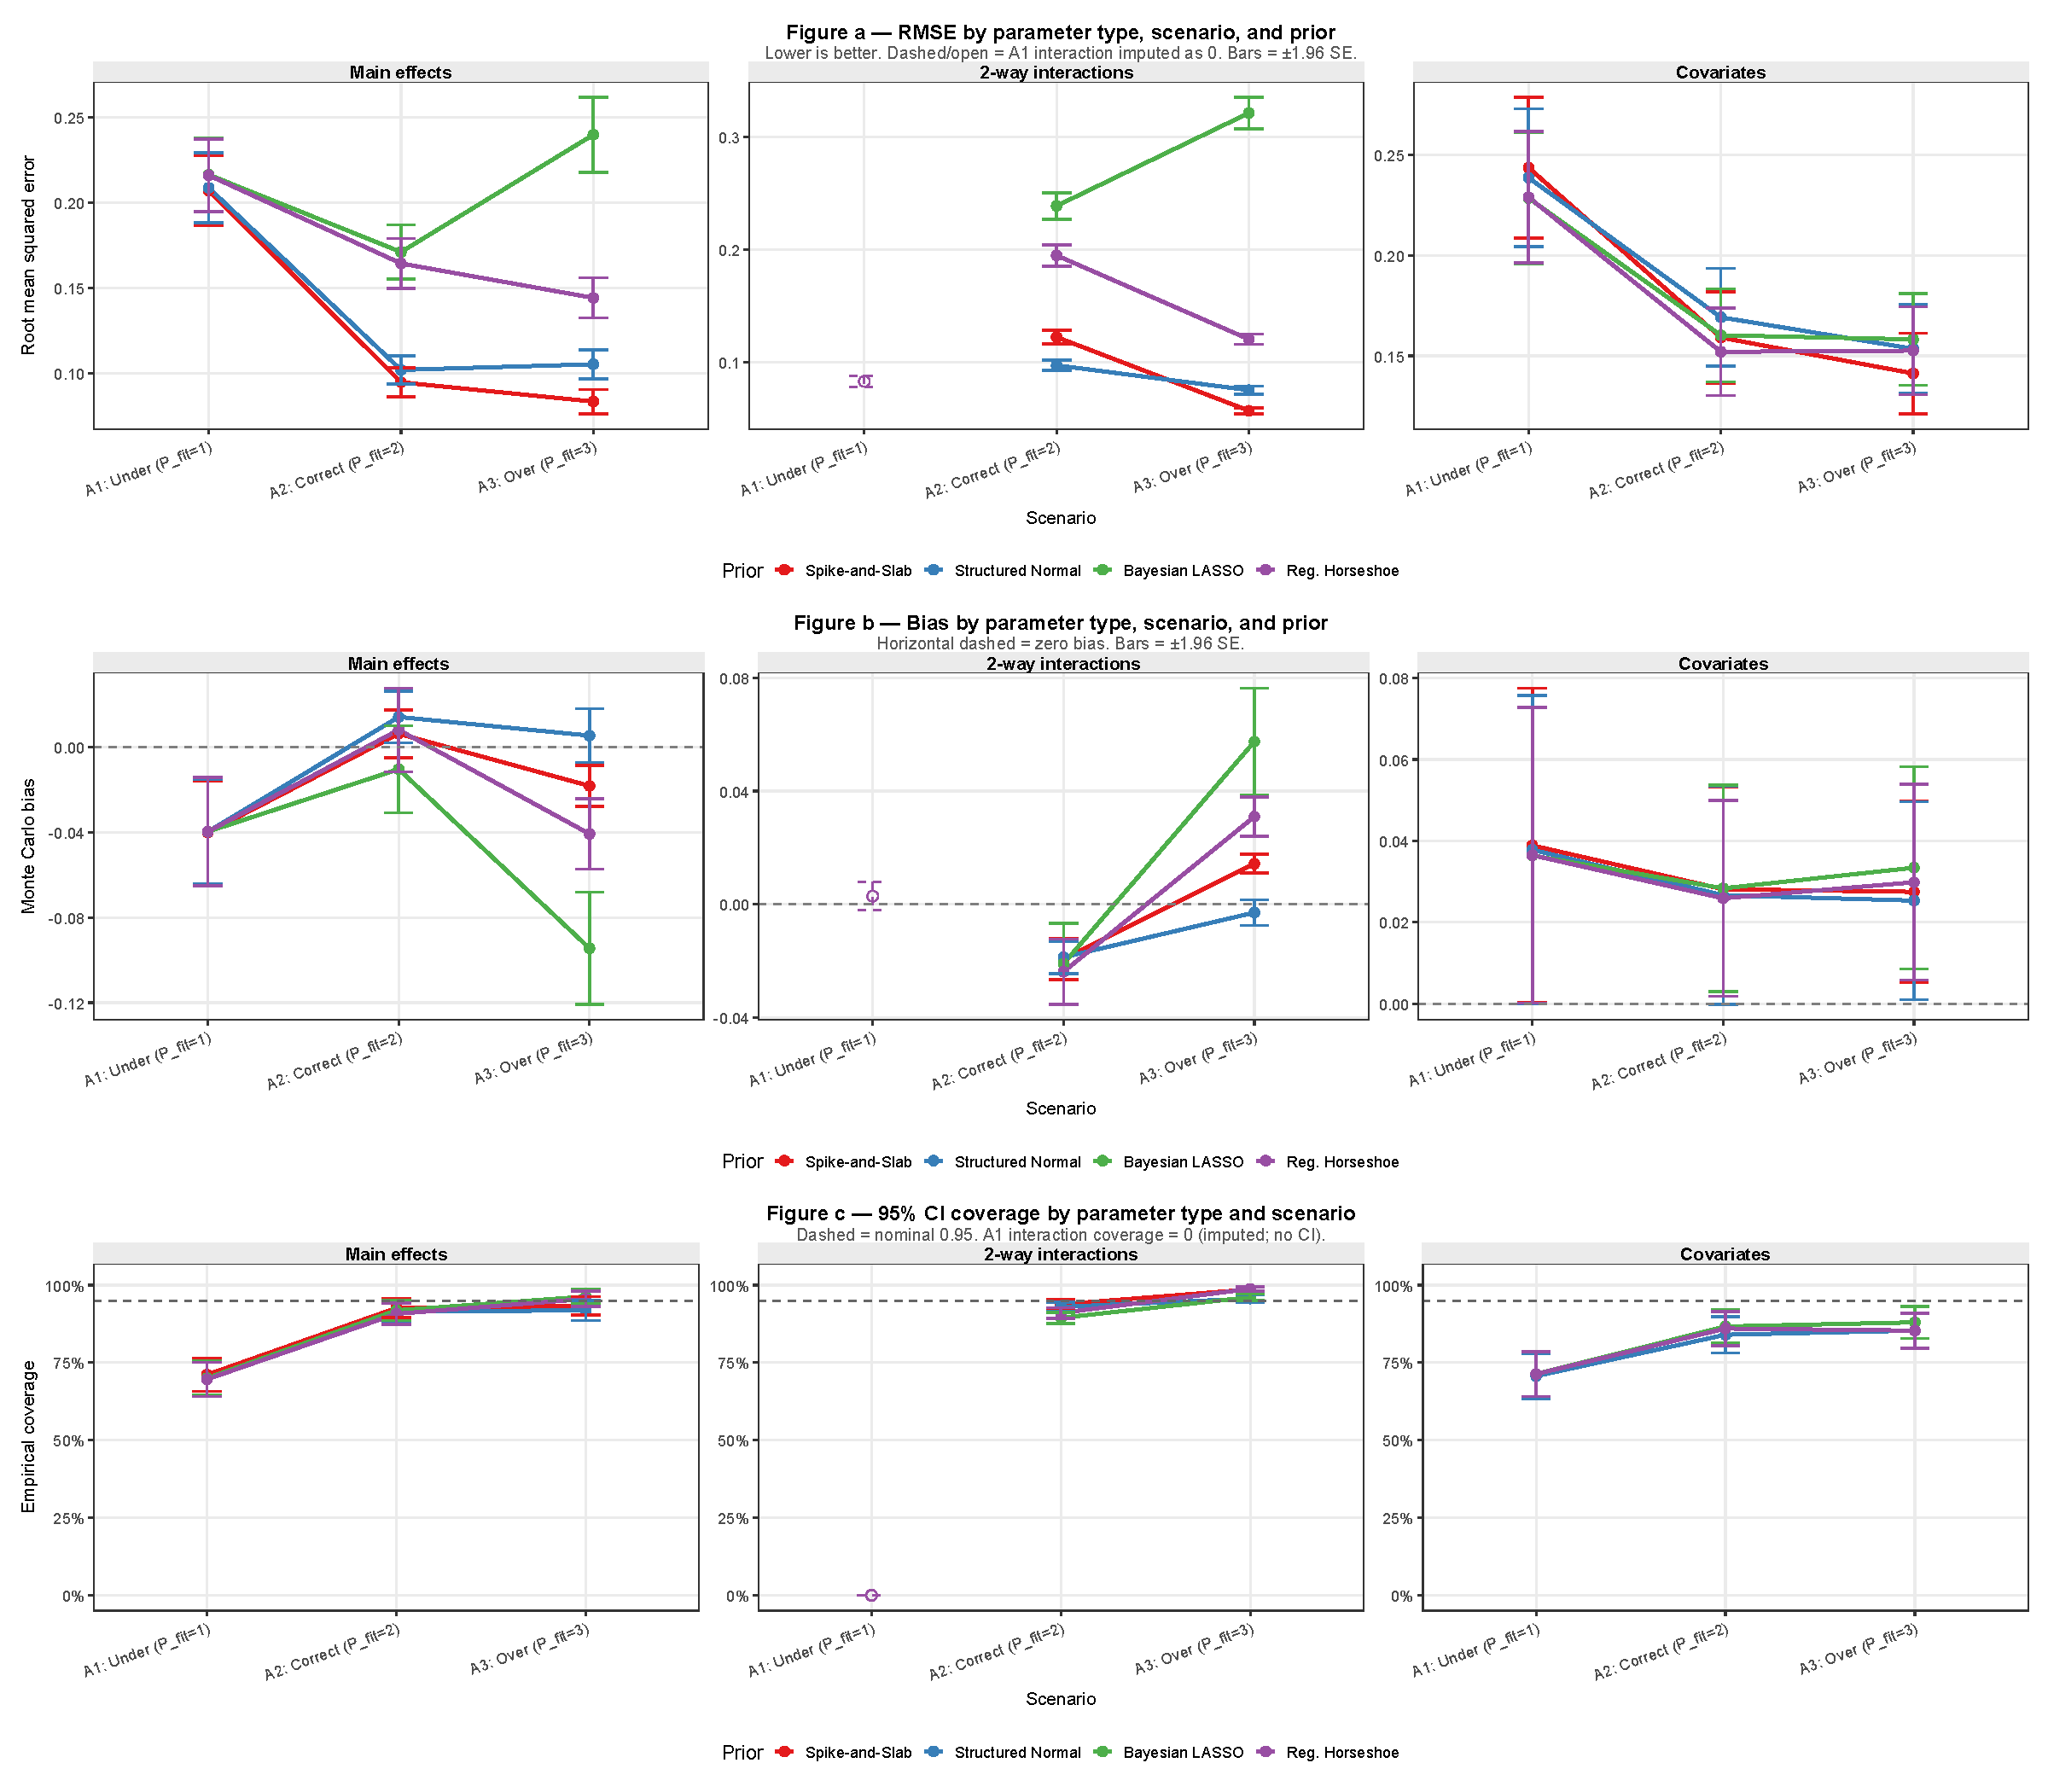
\includegraphics[width=\linewidth]{sim_results/figures/fig1_recovery_combined.pdf}
\caption{Coefficient recovery by type, analysis model, and prior.  \emph{Top}: RMSE
(lower is better).  \emph{Middle}: Monte Carlo bias; dashed line at zero.
\emph{Bottom}: empirical coverage of 95\% credible intervals; dashed line at
nominal 0.95 level.  Columns: main-effect coefficients ($\beta$), two-way interaction coefficients,
covariate coefficients ($\gamma$). A1, A2, A3 refer to the under-, correctly,
and over-specified analysis models of Section~\ref{sec:analysis_models}.}
\label{fig:bias_coverage}
\end{figure}

\subsubsection{Variable selection}
\label{sec:sim_selection}
Variable selection performance is reported using a uniform $0.5$ threshold on the posterior PIP (spike-and-slab) or pseudo-PIP $\widetilde{\mathrm{PIP}}_j = \mathbb{E}[1 - \kappa_j \mid \mathcal{D}]$ (HS, Bayesian LASSO, regularised horseshoe) for declaring an edge active, as defined in Section~\ref{sec:pseudo_pip} and the modified TPR/FPR formulae in Section~4.4. TPR, FPR, and selection AUC are computed separately for the main-effect and two-way interaction coefficients across the three analysis models and four priors (Figures~\ref{fig:selection} and \ref{fig:selection_auc}).

\paragraph{Main-effect coefficients.}
For main-effect selection, the regularised horseshoe achieves near-perfect TPR ($\approx 100\%$) across all three analysis models, but this comes at the cost of an 
equally near-perfect FPR ($\approx 100\%$): the posterior shrinkage factor $\kappa_j$ rarely exceeds the cutoff so essentially every coefficient is declared active. The spike-and-slab, by contrast, achieves moderate TPR ($\approx 75\text{--}80\%$) with substantially lower FPR ($\approx 15\%$ under A1, declining further under A2 and A3), reflecting a genuine trade-off between sensitivity and specificity. The structured normal and Bayesian LASSO follow a pattern similar to the regularised horseshoe, with near-100\% TPR accompanied by near-100\% FPR across all analysis models, confirming that continuous shrinkage priors without a discrete selection component cannot perform meaningful variable selection at this common threshold.

\paragraph{Two-way interaction coefficients.}
The distinction between prior families is most striking for two-way interaction selection. The regularised horseshoe again achieves near-100\% TPR under A2 and A3, but with near-100\% FPR, rendering its high sensitivity uninformative. The structured normal and Bayesian LASSO behave similarly, collapsing to the no-discrimination diagonal. The spike-and-slab is the only prior to achieve meaningful selection performance: under A2, it attains TPR $\approx 73\%$ with FPR $\approx 4\%$, representing a large separation between sensitivity and false discovery rate. Under A3, spike-and-slab TPR declines to approximately $33\%$, reflecting the increased difficulty of identifying true interactions within a larger candidate set, while FPR remains near zero ($\approx 1\%$), demonstrating that its selectivity is preserved under over-specification. Under A1, interaction TPR is zero by construction for all priors as no interaction coefficients are estimated.

\paragraph{Selection AUC.}
Figure~\ref{fig:selection_auc} confirms and clarifies the picture from Figure~\ref{fig:selection}. The regularised horseshoe achieves selection AUC $\approx 47\text{--}48\%$ for both the main-effect and two-way interaction coefficients across all analysis models---effectively at or below the random classifier baseline of $50\%$---confirming that its indiscriminate inclusion 
of all parameters yields no useful ranking of active versus inactive terms. In contrast, the spike-and-slab, structured normal, and Bayesian LASSO all achieve selection AUC in the range $85\text{--}95\%$ under A2 and A3 for both coefficient types, with the structured normal attaining the highest AUC under A3 for two-way interactions ($\approx 92\%$) and the Bayesian LASSO showing the greatest decline from A2 to A3. For the main-effect coefficients, all three non-horseshoe priors achieve comparable AUC improvement from A1 to A2, with the Bayesian LASSO showing a notable drop under A3 relative to A2. Taken together, the AUC results indicate that while the spike-and-slab uniquely controls FPR at the $0.5$ threshold, the structured normal and Bayesian LASSO retain competitive PIP ranking ability despite their inability to achieve sparse hard selection.

\begin{figure}[H]
\centering
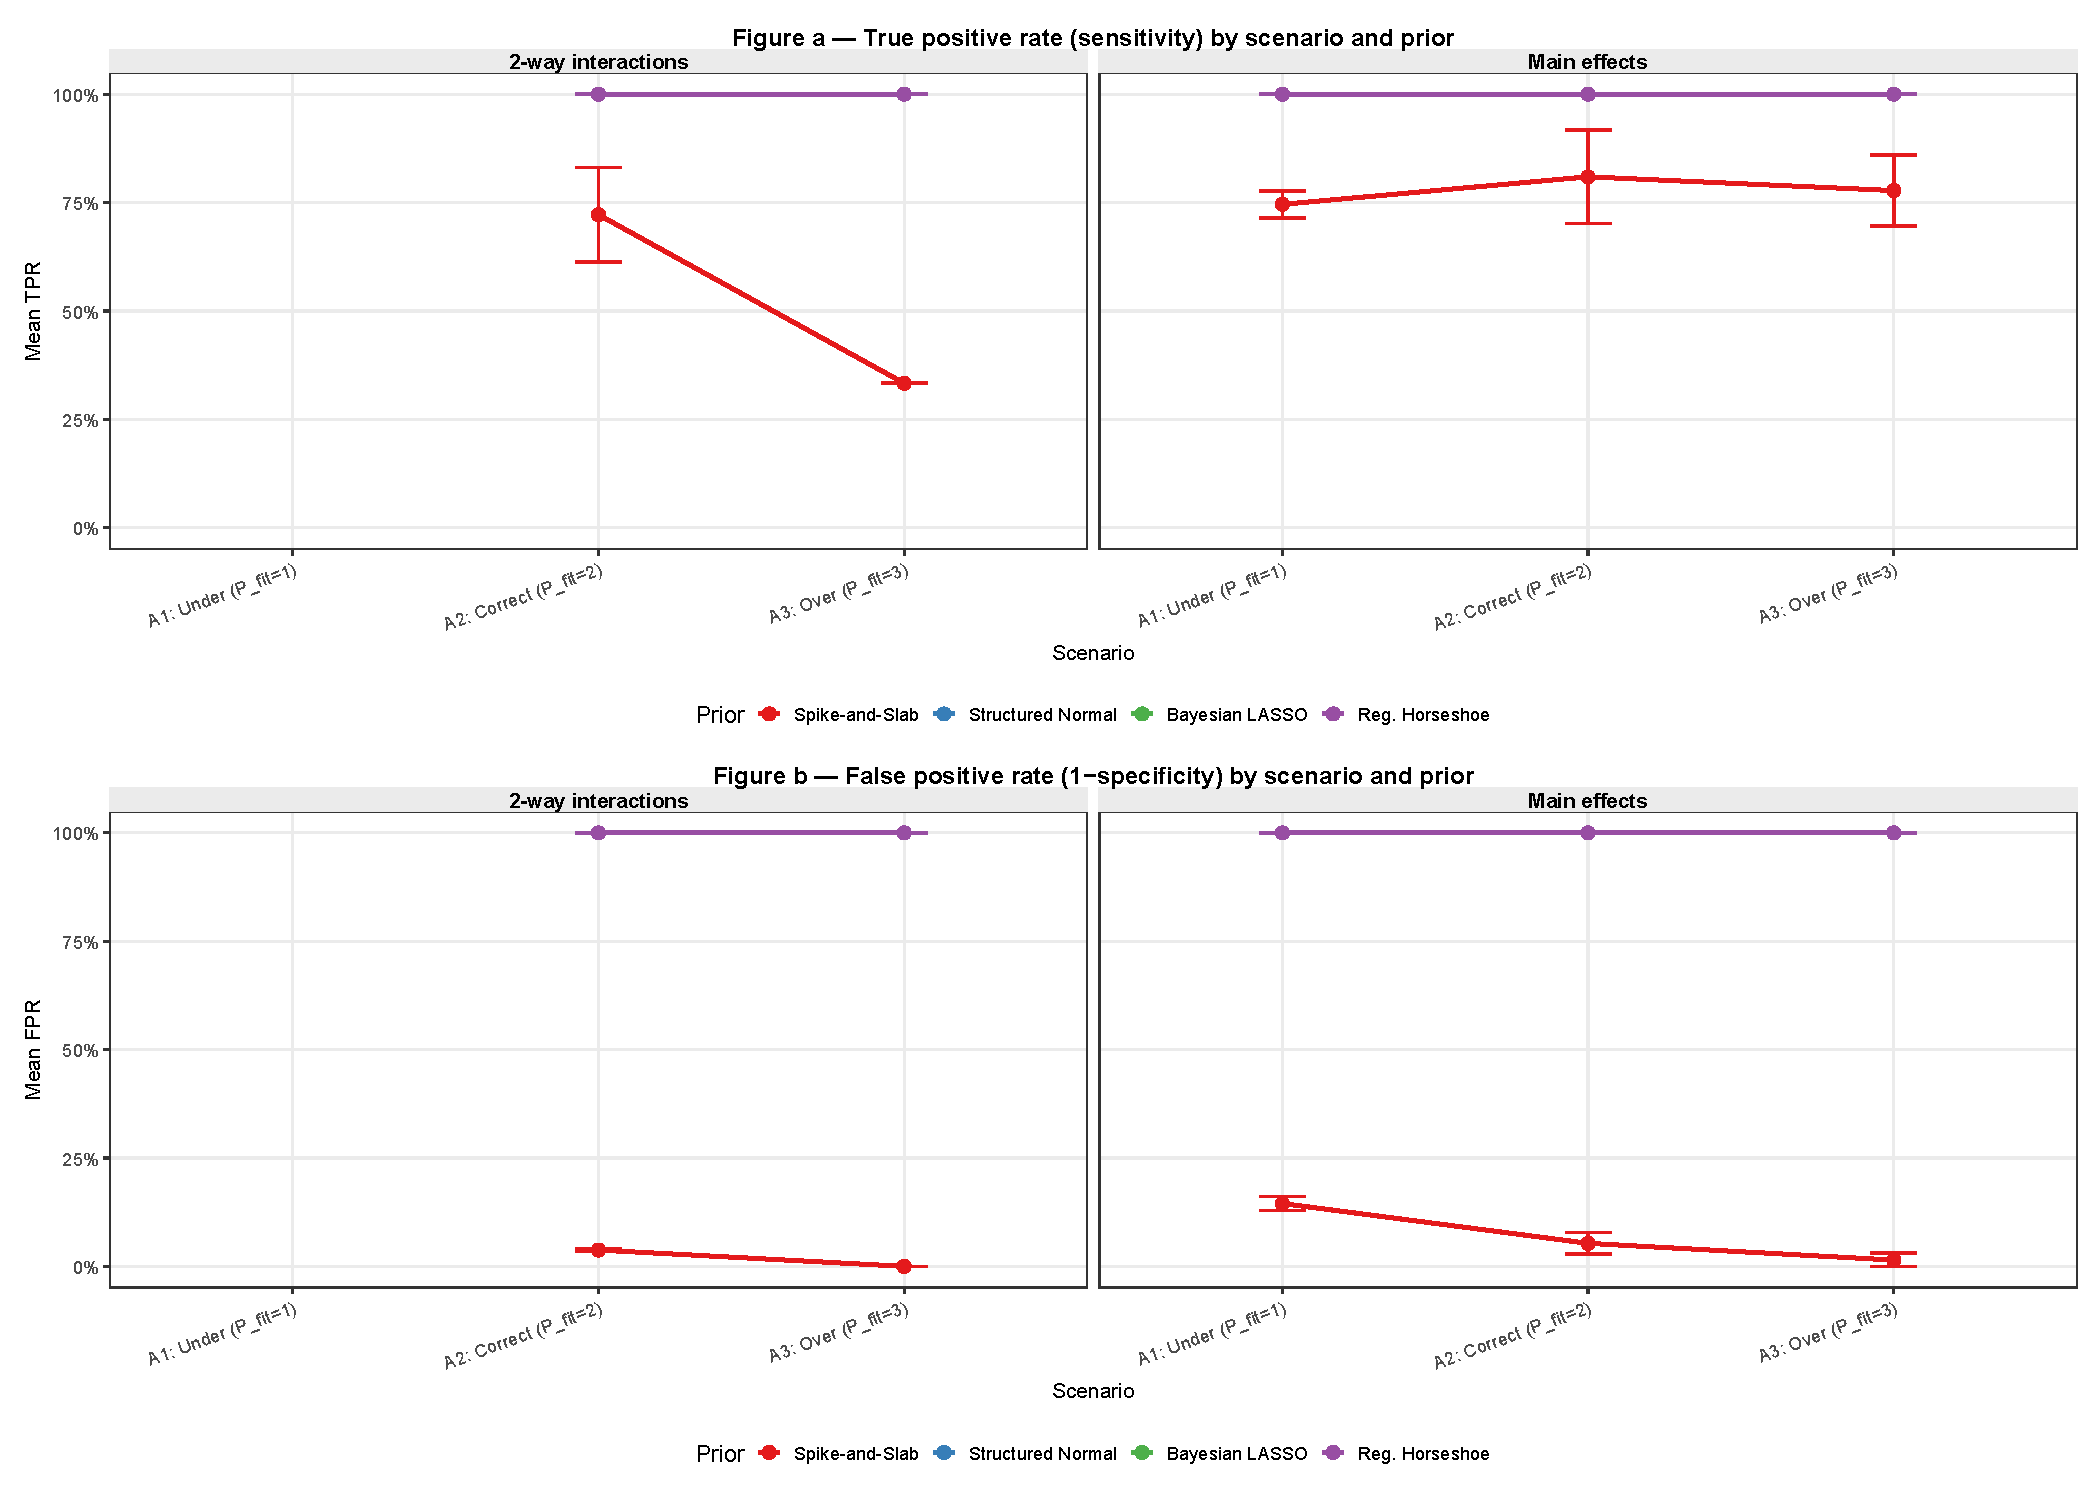
\includegraphics[width=\linewidth]{sim_results/figures/fig4_selection_tpr_fpr.pdf}
\caption{Variable selection performance by analysis model and prior, using a uniform $0.5$ threshold on the (pseudo-)PIP for all four priors.  \emph{Top row}:
TPR.  \emph{Bottom row}: FPR.  Left column: main-effect coefficients; right column: two-way interaction coefficients.
Error bars: $\pm1.96$\,SE across Monte Carlo replicates.}
\label{fig:selection}
\end{figure}

\begin{figure}[H]
\centering
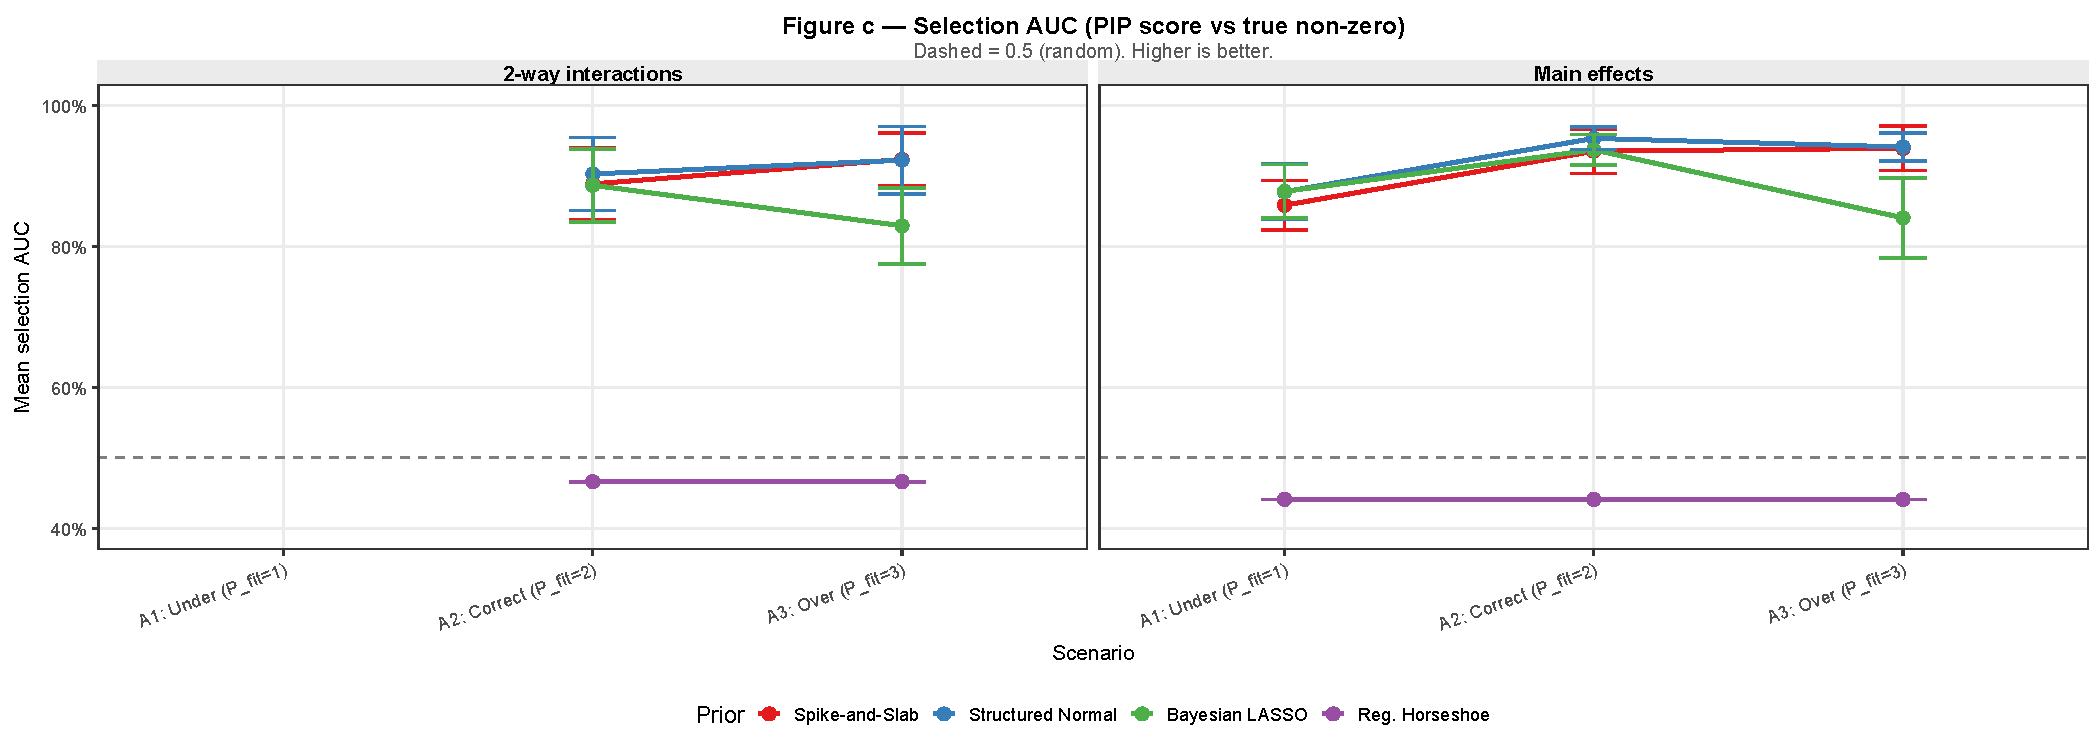
\includegraphics[width=\linewidth]{sim_results/figures/fig4c_selection_auc.pdf}
\caption{Selection AUC by analysis model, coefficient type, and prior.  Dashed line at
AUC\,$= 0.50$ (random discrimination).}
\label{fig:selection_auc}
\end{figure}

\subsubsection{Predictive performance and prior comparison summary}

Table~\ref{tab:pred_metrics} reports the Poisson log-likelihood and Brier score for each prior under each analysis model. The four priors are nearly indistinguishable on held-out prediction within each analysis model: under A2, Poisson log-likelihood ranges only from $-0.5726$ (spike-and-slab) to $-0.5731$ (Bayesian LASSO) and Brier scores span $0.1573$--$0.1576$. The under-specified analysis model A1 produces the largest degradation (Poisson LL $\approx -0.5746$, Brier $\approx 0.158$ for all priors), while the over-specified A3 is marginally better than A2 for most priors except the Bayesian LASSO, which shows mild deterioration consistent with its tendency to over-fit under an expanded parameter space. Oracle efficiency analysis (Brier ratio of fitted to oracle model; Appendix Figure~\ref{fig:oracle}) confirms that all four priors achieve oracle-level efficiency across all conditions and analysis models, with no systematic left-tail mass below $0.9$.

\begin{table}[H]
\centering
\caption{Predictive performance metrics across analysis models and prior families. Poisson log-likelihood (Pois.\ LL) and Brier score are averaged over simulation replicates; standard errors (SE) are shown in parentheses. Higher Poisson log-likelihood (less negative) and lower Brier score indicate better 
predictive performance. A1: under-specified ($P_{\mathrm{fit}}=1$, interaction terms omitted); A2: correctly specified ($P_{\mathrm{fit}}=2$); A3: over-specified ($P_{\mathrm{fit}}=3$, spurious higher-order terms included).} \label{tab:pred_metrics}
% latex table generated in R 4.5.0 by xtable 1.8-4 package
% Wed Apr 15 02:01:53 2026
\begin{tabular}{clcc}
\toprule
\multicolumn{1}{c}{Scenario} & \multicolumn{1}{c}{Prior} 
    & Pois.\ LL & Brier score \\
 & & \multicolumn{1}{c}{mean (SE)} & \multicolumn{1}{c}{mean (SE)} \\
\midrule
\multirow{4}{*}{A1: Under}
  & Spike-and-Slab       & $-0.5746$ $(0.0007)$ & $0.1582$ $(0.0002)$ \\
  & Structured Normal    & $-0.5746$ $(0.0007)$ & $0.1582$ $(0.0002)$ \\
  & Bayesian LASSO       & $-0.5746$ $(0.0007)$ & $0.1581$ $(0.0002)$ \\
  & Reg.\ Horseshoe      & $-0.5746$ $(0.0007)$ & $0.1581$ $(0.0002)$ \\
\midrule
\multirow{4}{*}{A2: Correct}
  & \textbf{Spike-and-Slab}    & $\mathbf{-0.5726}$ $(0.0007)$ & $0.1574$ $(0.0002)$ \\
  & Structured Normal          & $-0.5729$ $(0.0007)$ & $0.1576$ $(0.0002)$ \\
  & Bayesian LASSO             & $-0.5731$ $(0.0007)$ & $\mathbf{0.1573}$ $(0.0002)$ \\
  & Reg.\ Horseshoe            & $-0.5729$ $(0.0007)$ & $0.1574$ $(0.0002)$ \\
\midrule
\multirow{4}{*}{A3: Over}
  & \textbf{Spike-and-Slab}    & $\mathbf{-0.5721}$ $(0.0007)$ & $\mathbf{0.1572}$ $(0.0002)$ \\
  & Structured Normal          & $-0.5725$ $(0.0007)$ & $0.1574$ $(0.0002)$ \\
  & Bayesian LASSO             & $-0.5744$ $(0.0008)$ & $0.1574$ $(0.0002)$ \\
  & Reg.\ Horseshoe            & $-0.5725$ $(0.0007)$ & $\mathbf{0.1572}$ $(0.0002)$ \\
\bottomrule
\multicolumn{4}{l}{}
\end{tabular}

\end{table}

Combining parameter recovery, variable selection, and predictive metrics, the spike-and-slab presents the most coherent profile for network structure learning: it ranks first on RMSE, FPR, coverage calibration, and Poisson log-likelihood across all or most analysis models, at the cost of reduced TPR (rank 4) reflecting the conservatism of its hard-thresholding selection mechanism. The structured normal is a viable secondary choice when a continuous prior is preferred and hard selection is not required. The Bayesian LASSO ranks last on RMSE and FPR but achieves competitive predictive performance under A1 and A2; the regularised horseshoe is poor for variable selection (selection AUC $\approx 47\%$) despite competitive coverage and Brier score under A3 and so is not recommended where network structure recovery is the goal. A full rank-by-metric summary across analysis models is given in the prior ranking heatmap (Figure~\ref{fig:ranking_heatmap}); detailed per-prior commentary is provided in Supplementary Section~S3.

\begin{figure}[H]
\centering
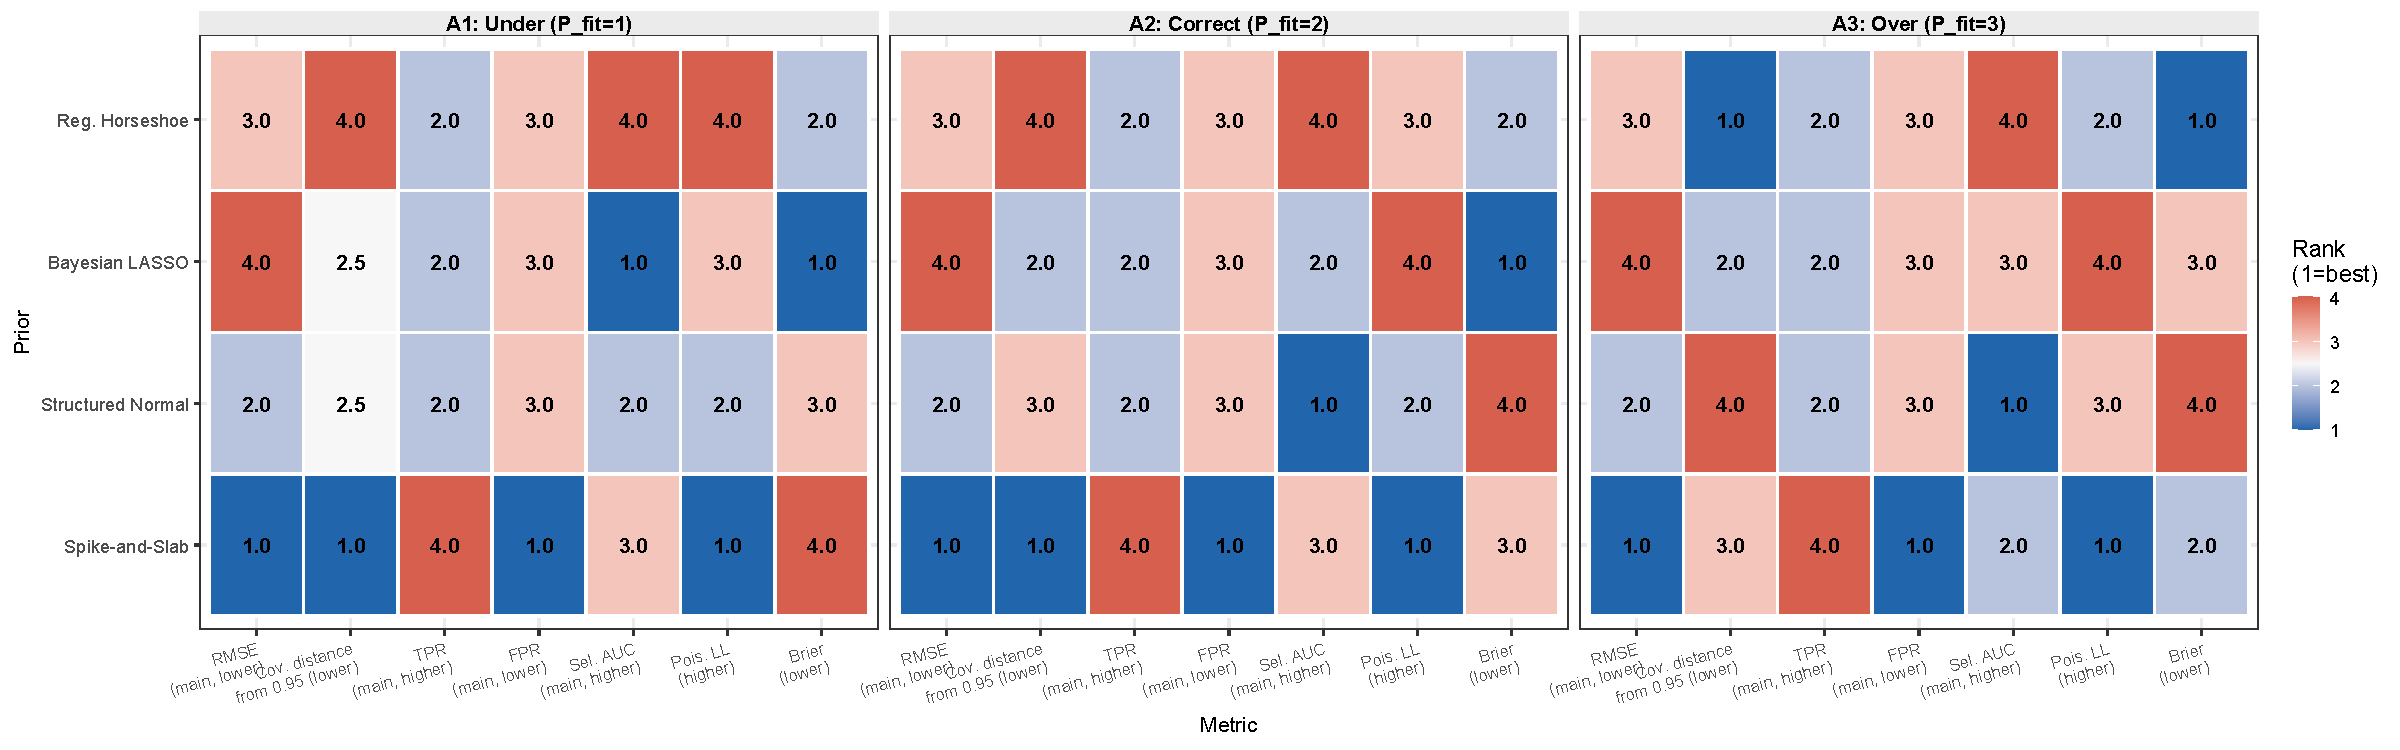
\includegraphics[width=\linewidth]{sim_results/figures/fig6_prior_ranking_heatmap.pdf}
\caption{Prior ranking heat-map by analysis model and metric.  Rank 1 (blue) = best;
Rank 4 (red) = worst.  Metrics: RMSE, coverage deviation from 0.95, TPR, FPR,
selection AUC, Poisson log-likelihood, Brier score.}
\label{fig:ranking_heatmap}
\end{figure}


%% ============================================================
\section{Discussion}
\label{sec:discussion}
%% ============================================================

\subsection{Summary of Main Findings}

This study demonstrates that a structured Bayesian continuous-time Bayesian 
network (CTBN) framework with order-dependent shrinkage priors can be applied 
to large-scale UK Biobank primary care EHR data to recover clinically plausible, 
sparse networks of multimorbidity progression. The recommended spike-and-slab 
model with pairwise interactions ($P = 2$) and penalty $\theta = 1$ identifies 
two dominant network modules: a cardiometabolic cluster anchored by strongly 
bidirectional edges among DM, HTN, and IHD ($\text{DM} \to \text{HTN}$: 
$\widehat{\text{RR}} = 2.13$, $+12.4$\,pp excess 5-year risk; 
$\text{HTN} \to \text{DM}$: $\widehat{\text{RR}} = 2.61$), and an inflammatory 
cluster characterised by dense within-cluster directed edges among RS, DE, and 
CLRD ($\text{CLRD} \to \text{RS}$: $\widehat{\text{RR}} = 2.09$; 
$\text{RS} \to \text{DE}$: $\widehat{\text{RR}} = 1.95$), consistent with 
shared atopic and airway-inflammatory mechanisms. Sparse but robust cross-cluster 
edges, notably $\text{OA} \to \text{RS}$ (PIP\,$= 0.92$) and 
$\text{OA} \to \text{DE}$ (PIP\,$= 0.96$), quantify inter-module pathways 
between musculoskeletal and inflammatory conditions.

Sub-multiplicative interactions, wherein the co-presence of two conditions 
attenuates the expected multiplicative hazard on a third, are concentrated 
entirely within the cardiometabolic cluster. All four active triplets 
($\text{PIP}_{jk}^{m} \geq 0.997$) exhibit sub-multiplicative antagonism 
(synergistic multiplier $< 1$), most prominently 
$\{\text{IHD}, \text{DM}\} \to \text{HTN}$ ($\Delta F_m(5) = \pm7.4$\,pp; 
synergistic multiplier $= 0.631$) and 
$\{\text{RS}, \text{DM}\} \to \text{HTN}$ ($\Delta F_m(5) = \pm7.7$\,pp; 
synergistic multiplier $= 0.646$), both meeting the \emph{clinically actionable} 
threshold. Simulation studies confirm that the spike-and-slab achieves the best 
RMSE, FPR control, coverage calibration, and Poisson log-likelihood among the 
four priors evaluated, at the cost of reduced sensitivity (TPR rank 4 across 
all analysis models); the regularised horseshoe, by contrast, provides no meaningful 
variable selection discrimination, achieving near-random selection AUC 
($\approx 47\text{--}48\%$) despite near-perfect TPR owing to indiscriminate 
parameter inclusion.

%% ------------------------------------------------------------
\subsection{Comparison with Related Work on Disease Networks}
%% ------------------------------------------------------------

The cardiometabolic network structure recovered here is broadly consistent with 
findings from large-scale multimorbidity studies. \citet{barnett2012epidemiology} 
identified diabetes, hypertension, and ischaemic heart disease as a persistent 
cluster in Scottish primary care, and our dynamic model adds directionality and 
quantifies the progression burden: diabetes is the most consequential existing 
condition, substantially accelerating both hypertension onset 
($\widehat{\text{RR}} = 2.13$, $+12.4$\,pp at 5 years) and IHD onset 
($\widehat{\text{RR}} = 1.40$, $+2.3$\,pp), consistent with the well-established 
role of insulin resistance in atherosclerotic and hypertensive disease. The 
temporal ordering implied by these directed edges aligns with the chronological 
atlas of \citet{kuan2019chronological}, who found that diabetes typically 
precedes hypertension and IHD in the sequence of morbidity accumulation in NHS 
data. The bidirectionality of the DM--HTN relationship 
($\text{HTN} \to \text{DM}$: $\widehat{\text{RR}} = 2.61$, $+3.4$\,pp) further 
reflects shared pathophysiological mechanisms, including renin--angiotensin 
system activation and glucocorticoid-mediated insulin resistance, that propagate 
risk in both directions over time.

The inflammatory cluster identified here extends this picture in ways that 
prior cross-sectional analyses have not quantified. The strong directed edge 
$\text{CLRD} \to \text{RS}$ ($\widehat{\text{RR}} = 2.09$, $+5.5$\,pp) and 
$\text{RS} \to \text{CLRD}$ ($\widehat{\text{RR}} = 1.79$, $+2.5$\,pp) confirm 
dense bidirectional reinforcement between upper and lower airway inflammatory 
disease, consistent with the atopic march hypothesis, by which chronic upper 
airway inflammation predisposes to lower airway disease through shared 
eosinophilic and Th2-mediated mechanisms \citep{cheng2024chronic, 
valabhji2024prevalence}. The $\text{RS} \to \text{DE}$ edge 
($\widehat{\text{RR}} = 1.95$, $+4.6$\,pp) similarly reflects the atopic triad 
of rhinitis, eczema, and asthma, a well-characterised immunological pathway 
\citep{yang2024longitudinal}. The cross-cluster edge $\text{OA} \to \text{RS}$ 
($\widehat{\text{RR}} \approx 1.36$, PIP\,$= 0.92$) represents a less 
well-characterised pathway; one plausible mechanism involves shared 
neuro-inflammatory sensitisation, though further mechanistic investigation is 
warranted.

The sub-multiplicative interaction findings carry direct clinical implications. 
All four active triplets involve conditions whose individual onset rates are 
already substantially elevated, and the sub-multiplicative synergistic 
multipliers (range $0.591$--$0.646$) indicate that their joint effect, while 
still substantially above baseline, is attenuated relative to the naive 
multiplicative expectation. The $\{\text{HTN}, \text{IHD}\} \to \text{DM}$ 
triplet exemplifies this most strikingly: despite the largest individual rate 
ratios ($\widehat{\text{RR}}_j = 2.610$, $\widehat{\text{RR}}_k = 2.011$), 
the synergistic multiplier of $0.591$ produces the smallest synergistic excess 
($\pm1.1$\,pp), consistent with a risk ceiling in patients with already 
severely compromised cardiometabolic profiles. These findings are consistent 
with evidence that metabolic syndrome constituents act on overlapping 
pathophysiological pathways, reducing the marginal contribution of each 
additional condition once the shared mechanisms are already saturated, as 
discussed in prospective cohort studies reviewed by 
\citet{valabhji2024prevalence}.

%% ------------------------------------------------------------
\subsection{Comparison with Related Methodological Work}
%% ------------------------------------------------------------

Comparing our approach with \citet{faruqui2021functional}, several key 
methodological advances are evident. First, we provide full posterior 
uncertainty quantification including credible intervals and PIPs, whereas 
\citet{faruqui2021functional} used frequentist $L_1$-regularisation with 
cross-validated penalty selection, which precludes formal probabilistic 
inference on edge inclusion. Second, our structured order-dependent shrinkage 
enables simultaneous estimation of main effects and pairwise interactions while 
preventing overfitting; simulation confirms that the spike-and-slab attains 
TPR $\approx 73\%$ for pairwise interactions at FPR $\approx 4\%$ under correct 
specification, a substantial improvement in precision-recall balance over 
continuous shrinkage alternatives that collapse to near-100\% TPR and FPR 
simultaneously. Third, our application to 33,558 UK Biobank participants 
substantially exceeds the scale of previous CTBN EHR analyses and simultaneously 
models ten conditions rather than three.

In comparison with the non-parametric Bayesian CTBN of \citet{yang2016learning, lasserre2021constraint}, 
our parametric log-linear approach does not sacrifices flexibility for interpretability 
and computational tractability. For the large-cohort EHR setting where clinical interpretability is essential, the our parametric model is preferable. However, the non-parametric approach would be warranted if exploratory analysis suggested 
substantial non-linearity in the intensity covariate relationship.

The comparison of our four priors provides nuanced insights aligned with 
theoretical predictions. The spike-and-slab's dominance for parameter recovery, 
FPR control, and coverage calibration corroborates \citet{bhadra2019lasso}, who 
showed that explicit zero-probability spike components outperform continuous 
shrinkage for variable selection under moderate-to-high true sparsity. The 
horseshoe's near-random selection AUC ($\approx 47\%$, below the random 
classifier baseline of $50\%$) is consistent with \citet{piironen2017sparsity}'s 
observation that the regularised horseshoe controls the effective number of 
parameters globally but does not provide posterior variable selection at the 
individual coefficient level without additional thresholding; in our simulation, 
this manifests as indiscriminate PIP assignment across active and inactive 
parameters. The competitive predictive performance of all four priors under 
correct specification is consistent with the well-known insensitivity of 
predictive accuracy to prior specification \citep{VehtariGelmanGabry2017}, and 
is confirmed here by the near-identical Poisson log-likelihood and Brier scores 
across priors within each analysis model (Table~\ref{tab:pred_metrics}).

The confirmation of GlycA and haematological biomarkers (neutrophil, lymphocyte, 
WBC) as high-PIP predictors adds to growing evidence that composite 
glycoprotein NMR biomarkers and systemic inflammatory indices capture 
cardiometabolic risk beyond CRP \citep{cheng2024chronic}. Albumin's 
consistent protective association across all ten conditions, with reduced onset 
rates uniformly observed, is consistent with its established role as an 
integrated marker of nutritional status and systemic inflammatory burden. 
Similarly, GlycA's selection for cardiometabolic targets (HTN and DM) 
corroborates evidence linking chronic low-grade inflammation to insulin 
resistance and endothelial dysfunction.

%% ------------------------------------------------------------
\subsection{Limitations}
%% ------------------------------------------------------------

Several limitations merit consideration. First, the log-linear CTBN assumes piecewise-constant intensities over at-risk intervals, precluding smooth hazard 
functions; non-parametric extensions could relax this assumption at additional computational cost. Second, the absorbing-state assumption may not hold for 
conditions characterised by relapse--remission cycles (e.g.\ rhinitis, dermatitis). Third, the UK Biobank cohort is not fully representative of the general UK population due to healthy volunteer bias; 
caution is warranted in generalising absolute incidence estimates to population-level projections. Fourth, the sub-multiplicative interaction 
findings, while statistically well-supported (PIP $\geq 0.997$), require external replication in independent cohorts before informing clinical decision 
rules, as the interaction parameter estimates are sensitive to the correctness of the multiplicative baseline model. Fifth, the time-dependent AUC reported here uses the inverse-probability-of-censoring weighted estimator of \citet{BlancheCommengesJacqmin-Gadda2013}; because the CTBN itself is a generative model for event times, a fully Bayesian alternative would impute event times for censored patients from the posterior predictive distribution and compute the AUC on the imputed complete data, avoiding the need for IPCW weights and propagating posterior uncertainty into the AUC directly. Implementing and benchmarking this Bayesian-imputation AUC against the IPCW estimator is a natural extension for future work.

%% ============================================================
\section{Conclusion and Recommendations}
\label{sec:conclusion}
%% ============================================================

This paper has presented and evaluated a structured Bayesian CTBN framework for modelling multimorbidity trajectories in large-scale electronic health 
records, with four alternative order-dependent shrinkage priors compared through simulation and applied to UK Biobank primary care data.

The principal substantive findings are: (i) the cardiometabolic cluster, anchored by diabetes as the most consequential existing condition, is the 
dominant feature of the multimorbidity network, with 
$\widehat{\text{RR}} = 2.13$ and $+12.4$\,pp excess 5-year risk for $\text{DM} \to \text{HTN}$, and a strongly bidirectional relationship with 
HTN ($\widehat{\text{RR}} = 2.61$ in the reverse direction); (ii) the inflammatory cluster---Rhinitis/Sinusitis, Dermatitis/Eczema, and Chronic 
Lower Respiratory Disease---forms a coherent module with dense within-cluster directed edges consistent with atopic and airway-inflammatory mechanisms, led 
by $\text{CLRD} \to \text{RS}$ ($\widehat{\text{RR}} = 2.09$, $+5.5$\,pp) and $\text{RS} \to \text{DE}$ ($\widehat{\text{RR}} = 1.95$, $+4.6$\,pp); 
(iii) sparse but well-supported cross-cluster edges, particularly from OA to the inflammatory conditions and from MN to HL, quantify inter-module 
pathways at clinically meaningful excess risk magnitudes; (iv) all four active high-PIP triplets exhibit sub-multiplicative antagonism concentrated 
within the cardiometabolic cluster, with the largest synergistic excess observed for $\{\text{RS}, \text{DM}\} \to \text{HTN}$ ($\pm7.7$\,pp) and 
$\{\text{IHD}, \text{DM}\} \to \text{HTN}$ ($\pm7.4$\,pp); and (v) age, smoking, BMI, GlycA, haematological markers (neutrophil, lymphocyte, WBC), 
and albumin are confirmed predictors with high PIPs, with albumin emerging as the most consistent protective factor across all ten conditions.

Among the four priors evaluated, the continuous spike-and-slab with $P = 2$ and $\theta = 1$ is recommended as the primary specification for network analysis. This recommendation is supported by its leading performance on RMSE, FPR control, coverage calibration, and Poisson log-likelihood across all analysis models, its capacity to deliver interpretable PIPs with meaningful discrimination between active and inactive parameters (selection 
AUC $\approx 85\text{--}92\%$ vs.\ near-random for the regularised horseshoe), and its robustness to model order misspecification under A3. The regularised 
horseshoe is not recommended for variable selection in this setting, as its selection AUC falls below the random classifier baseline; it may however retain value as a predictive model where point estimation rather than network structure recovery is the goal. The structured normal is a viable secondary 
choice when computational considerations favour a continuous prior and hard variable selection is not required.

In conclusion, the structured Bayesian CTBN framework presented here provides a principled, scalable, and clinically interpretable approach to modelling 
multimorbidity trajectories in large-scale EHR data. The simulation evidence establishes the spike-and-slab prior as the preferred specification for network structure recovery across all three analysis models, while the empirical application to UK Biobank demonstrates that the recovered network is both statistically robust and clinically coherent, recovering known cardiometabolic and atopic pathways while providing novel quantification of their magnitude, directionality, and interactive structure. The extension of this framework to the full 60-condition InflAim project represents a significant methodological advance in population-scale disease network modelling, with direct applications to prevention, risk stratification, and precision medicine for individuals with complex multimorbidity.

%% ============================================================
\section*{Code and Data Availability}
%% ============================================================
\addcontentsline{toc}{section}{Code and Data Availability}

All Stan code, R scripts for simulation and empirical analysis, and post-processing pipelines for figures and tables are available at the following GitHub repository: \url{https://github.com/InflAim/CTBN-Multimorbidity}. The repository includes (i) Stan model files for each of the four shrinkage priors (spike-and-slab, hierarchical structured, Bayesian LASSO, and regularised horseshoe); (ii) R scripts for converting raw EHR records to the at-risk interval format used by the CTBN; (iii) simulation scripts for reproducing all three analysis models (A1, A2, A3); and (iv) plotting code for all figures in this paper and its Supplementary Material. UK Biobank primary care data are not publicly available but can be accessed by approved researchers through the UK Biobank Access Management System (\url{https://www.ukbiobank.ac.uk/}).

%% ============================================================
\section*{Acknowledgements}
%% ============================================================
\addcontentsline{toc}{section}{Acknowledgements}

This research was conducted using the UK Biobank Resource under approved application. We thank UK Biobank participants and the InflAim consortium for support of the broader research programme.

%% ============================================================
\bibliographystyle{apalike}
\bibliography{reference}
%% ============================================================

\newpage
%% ============================================================
\appendix
\section*{Appendix}
%% ============================================================

\setcounter{section}{0}
\renewcommand{\thesection}{A\arabic{section}}
\renewcommand{\thetable}{A\arabic{table}}
\renewcommand{\thefigure}{A\arabic{figure}}
\setcounter{table}{0}
\setcounter{figure}{0}

\section{Consort diagram}

\begin{figure}[H]
\centering

\includegraphics[width=1\linewidth]{inflAim_consort_diagram_v2.png}
\caption{InflAim Study Cohort Selection Flow Diagram}
\label{fig:consort}
\end{figure}

%\section{Supplementary Tables: Simulation Study}

%\begin{table}[H]
%\scriptsize
%\centering
%\caption{Master performance summary across all priors, scenarios, and metrics.}
%\label{tab:master}
%% latex table generated in R 4.5.0 by xtable 1.8-4 package
% Wed Apr 15 02:01:59 2026
\begin{tabular}{lllllllll}
  \hline
Scenario & Prior & RMSE (main) & Coverage (main) & TPR (main) & FPR (main) & Sel. AUC (main) & Pois. LL & Brier \\ 
  \hline
A1 & Spike-and-Slab & 0.2072 & 0.711 & 0.746 & 0.145 & 0.858 & -0.5746 & 0.1582 \\ 
  A1 & Structured Normal & 0.2088 & 0.700 & 1.000 & 1.000 & 0.877 & -0.5746 & 0.1582 \\ 
  A1 & Bayesian LASSO & 0.2165 & 0.700 & 1.000 & 1.000 & 0.878 & -0.5746 & 0.1581 \\ 
  A1 & Reg. Horseshoe & 0.2161 & 0.696 & 1.000 & 1.000 & 0.441 & -0.5746 & 0.1581 \\ 
  A2 & Spike-and-Slab & 0.0949 & 0.926 & 0.810 & 0.053 & 0.935 & -0.5726 & 0.1574 \\ 
  A2 & Structured Normal & 0.1021 & 0.915 & 1.000 & 1.000 & 0.953 & -0.5729 & 0.1576 \\ 
  A2 & Bayesian LASSO & 0.1712 & 0.919 & 1.000 & 1.000 & 0.937 & -0.5731 & 0.1573 \\ 
  A2 & Reg. Horseshoe & 0.1645 & 0.907 & 1.000 & 1.000 & 0.441 & -0.5729 & 0.1574 \\ 
  A3 & Spike-and-Slab & 0.0836 & 0.933 & 0.778 & 0.014 & 0.939 & -0.5721 & 0.1572 \\ 
  A3 & Structured Normal & 0.1054 & 0.919 & 1.000 & 1.000 & 0.941 & -0.5725 & 0.1574 \\ 
  A3 & Bayesian LASSO & 0.2399 & 0.963 & 1.000 & 1.000 & 0.840 & -0.5744 & 0.1574 \\ 
  A3 & Reg. Horseshoe & 0.1443 & 0.956 & 1.000 & 1.000 & 0.441 & -0.5725 & 0.1572 \\ 
   \hline
\end{tabular}

%\end{table}

\clearpage
\section{Supplementary Tables: Empirical Analysis}

\begin{table}[htbp]
\small
\centering
\caption{Mean and Standard Error (SE) of Brier score and Poisson LL by prior family and
interaction order.}
\label{tab:order_performance}
% latex table generated in R 4.5.0 by xtable 1.8-4 package
% Wed Apr 15 01:02:12 2026
%\small
\begin{tabular}{llcc}
\toprule
\multicolumn{1}{c}{Prior} & 
\multicolumn{1}{c}{$P$} & 
Brier score & 
Poisson LL \\
& & mean (SE) & mean (SE) \\
\midrule
\multirow{3}{*}{Spike-and-Slab}
  & 1 & $0.0635$ $(0.0025)$ & $-0.2651$ $(0.0080)$ \\
  & 2 & $0.0635$ $(0.0025)$ & $-0.2651$ $(0.0080)$ \\
  & 3 & $0.0635$ $(0.0025)$ & $-0.2651$ $(0.0080)$ \\
\midrule
\multirow{3}{*}{Structured Normal}
  & 1 & $0.0635$ $(0.0025)$ & $-0.2652$ $(0.0080)$ \\
  & 2 & $0.0635$ $(0.0025)$ & $-0.2652$ $(0.0080)$ \\
  & 3 & $0.0635$ $(0.0025)$ & $-0.2652$ $(0.0080)$ \\
\midrule
\multirow{3}{*}{Bayesian LASSO}
  & 1 & $0.0635$ $(0.0025)$ & $-0.2652$ $(0.0080)$ \\
  & 2 & $0.0635$ $(0.0025)$ & $-0.2652$ $(0.0080)$ \\
  & 3 & $0.0635$ $(0.0025)$ & $-0.2654$ $(0.0080)$ \\
\midrule
\multirow{3}{*}{Reg.\ Horseshoe}
  & 1 & $0.0635$ $(0.0025)$ & $-0.2652$ $(0.0080)$ \\
  & 2 & $0.0635$ $(0.0025)$ & $-0.2652$ $(0.0080)$ \\
  & 3 & $0.0635$ $(0.0025)$ & $-0.2652$ $(0.0080)$ \\
\bottomrule
\multicolumn{4}{l}{}
\end{tabular}

\end{table}


\begin{table}[htbp]
\small
\centering
\caption{Active edges (PIP $\geq 0.50$), ordered by PIP.
* = at least one node in the inflammatory cluster.}
\label{tab:network_edges}
% latex table generated in R 4.5.0 by xtable 1.8-4 package
% Wed Apr 15 00:39:00 2026
\begin{tabular}{lllllll}
  \hline
Influencer & Target & \mbox{[Infl]}* & PIP & log RR & RR & q0 (/1kpy) \\ 
  \hline
HTN & IHD &  & 1.000 & 0.5113 & 1.668 & 12.52 \\ 
  HTN & DM &  & 1.000 & 0.9593 & 2.610 & 4.34 \\ 
  IHD & DM &  & 1.000 & 0.6986 & 2.011 & 4.34 \\ 
  \mbox{[Infl]} RS & \mbox{[Infl]} DE & * & 1.000 & 0.6655 & 1.945 & 10.46 \\ 
  \mbox{[Infl]} RS & \mbox{[Infl]} CLRD & * & 1.000 & 0.5800 & 1.786 & 6.59 \\ 
  \mbox{[Infl]} DE & \mbox{[Infl]} RS & * & 1.000 & 0.5319 & 1.702 & 11.02 \\ 
  MN & DVL &  & 1.000 & 0.5534 & 1.739 & 6.17 \\ 
  \mbox{[Infl]} CLRD & \mbox{[Infl]} RS & * & 1.000 & 0.7352 & 2.086 & 11.02 \\ 
  DM & HTN &  & 1.000 & 0.7554 & 2.129 & 27.06 \\ 
  HL & IHD &  & 1.000 & 0.5543 & 1.741 & 12.52 \\ 
  DVL & \mbox{[Infl]} DE & * & 0.998 & 0.4138 & 1.513 & 10.46 \\ 
  \mbox{[Infl]} DE & DVL & * & 0.996 & 0.3988 & 1.490 & 6.17 \\ 
  \mbox{[Infl]} CLRD & \mbox{[Infl]} DE & * & 0.993 & 0.3827 & 1.466 & 10.46 \\ 
  IHD & HL &  & 0.980 & 0.3539 & 1.425 & 6.89 \\ 
  DM & IHD &  & 0.965 & 0.3368 & 1.400 & 12.52 \\ 
  OA & \mbox{[Infl]} DE & * & 0.960 & 0.3331 & 1.395 & 10.46 \\ 
  \mbox{[Infl]} RS & OA & * & 0.949 & 0.3249 & 1.384 & 9.29 \\ 
  \mbox{[Infl]} RS & HL & * & 0.944 & 0.3221 & 1.380 & 6.89 \\ 
  OA & \mbox{[Infl]} RS & * & 0.915 & 0.3076 & 1.360 & 11.02 \\ 
  MN & \mbox{[Infl]} DE & * & 0.849 & 0.2853 & 1.330 & 10.46 \\ 
  IHD & HTN &  & 0.777 & 0.2677 & 1.307 & 27.06 \\ 
  HL & \mbox{[Infl]} DE & * & 0.628 & 0.2390 & 1.270 & 10.46 \\ 
  \mbox{[Infl]} DE & HL & * & 0.623 & 0.2380 & 1.269 & 6.89 \\ 
  HTN & OA &  & 0.516 & 0.2187 & 1.244 & 9.29 \\ 
   \hline
\end{tabular}

\end{table}

\begin{table}[htbp]
\centering
\caption{Top 15 condition pairs by 5-year excess cumulative incidence.
* = at least one inflammatory condition.}
\label{tab:conditional_risk}
% latex table generated in R 4.5.0 by xtable 1.8-4 package
% Wed Apr 15 00:39:03 2026
%\small
\begin{tabular}{llcccccc}
\toprule
\textbf{Existing} & \textbf{Target} & \textbf{Infl.} & \textbf{Baseline (\%)} & \textbf{Conditional (\%)} & \textbf{Excess (\%)} & \textbf{RR} \\
\midrule
DM & HTN &  & 12.6 & 25.0 & +12.4 & 2.13 \\
CLRD & RS & * & 5.4 & 10.9 & +5.5 & 2.09 \\
RS & DE & * & 5.1 & 9.7 & +4.6 & 1.95 \\
HL & IHD &  & 6.1 & 10.3 & +4.2 & 1.74 \\
HTN & IHD &  & 6.1 & 9.9 & +3.8 & 1.67 \\
DE & RS & * & 5.4 & 8.9 & +3.6 & 1.70 \\
IHD & HTN &  & 12.6 & 16.2 & +3.5 & 1.31 \\
HTN & DM &  & 2.1 & 5.5 & +3.4 & 2.61 \\
DVL & DE & * & 5.1 & 7.6 & +2.5 & 1.51 \\
RS & CLRD & * & 3.2 & 5.7 & +2.5 & 1.79 \\
DM & IHD &  & 6.1 & 8.4 & +2.3 & 1.40 \\
CLRD & DE & * & 5.1 & 7.4 & +2.3 & 1.47 \\
CLRD & HTN & * & 12.6 & 14.9 & +2.2 & 1.19 \\
MN & DVL &  & 3.0 & 5.2 & +2.2 & 1.74 \\
IHD & DM &  & 2.1 & 4.3 & +2.1 & 2.01 \\
\bottomrule
\end{tabular}

\end{table}

\begin{table}[htbp]
\centering
\caption{Pairwise interaction decomposition for significant triplets (PIP$_{jk} \geq 0.50$; 5-year horizon).  * = inflammatory condition involved. Abbreviations: DM = Diabetes; HTN = Hypertensive diseases; IHD = Ischaemic heart diseases; RS = Rhinitis and sinusitis}
\label{tab:interaction_decomp}
% latex table generated in R 4.5.0 by xtable 1.8-4 package
% Wed Apr 15 00:39:03 2026
%\footnotesize
\begin{tabular}{lllcccccc}
\toprule
\textbf{Target} & \textbf{Cond. $j$} & \textbf{Cond. $k$} & \textbf{Infl.} & \textbf{RR ($j,k$)} & \textbf{Syn.} & \textbf{Joint RR} & $\boldsymbol{\Delta F_m(5)}$ & $\mathbf{PIP}$ \\
\midrule
DM  & HTN & IHD &  & (2.61, 2.01) & 0.591 & 3.099 & $\pm 1.1\%$ & 1.000 \\
IHD & HTN & DM  &  & (1.67, 1.40) & 0.642 & 1.498 & $\pm 3.3\%$ & 0.998 \\
HTN & IHD & DM  &  & (1.31, 2.13) & 0.631 & 1.755 & $\pm 7.4\%$ & 0.999 \\
HTN & RS  & DM  & * & (1.08, 2.13) & 0.646 & 1.491 & $\pm 7.7\%$ & 0.997 \\
\bottomrule
\end{tabular}

\end{table}


\clearpage
\section{Supplementary Figures}

%%%%%%%%%%%%%% Empirical Analysis Supplementary Figures %%%%%

\begin{figure}[H]
\centering
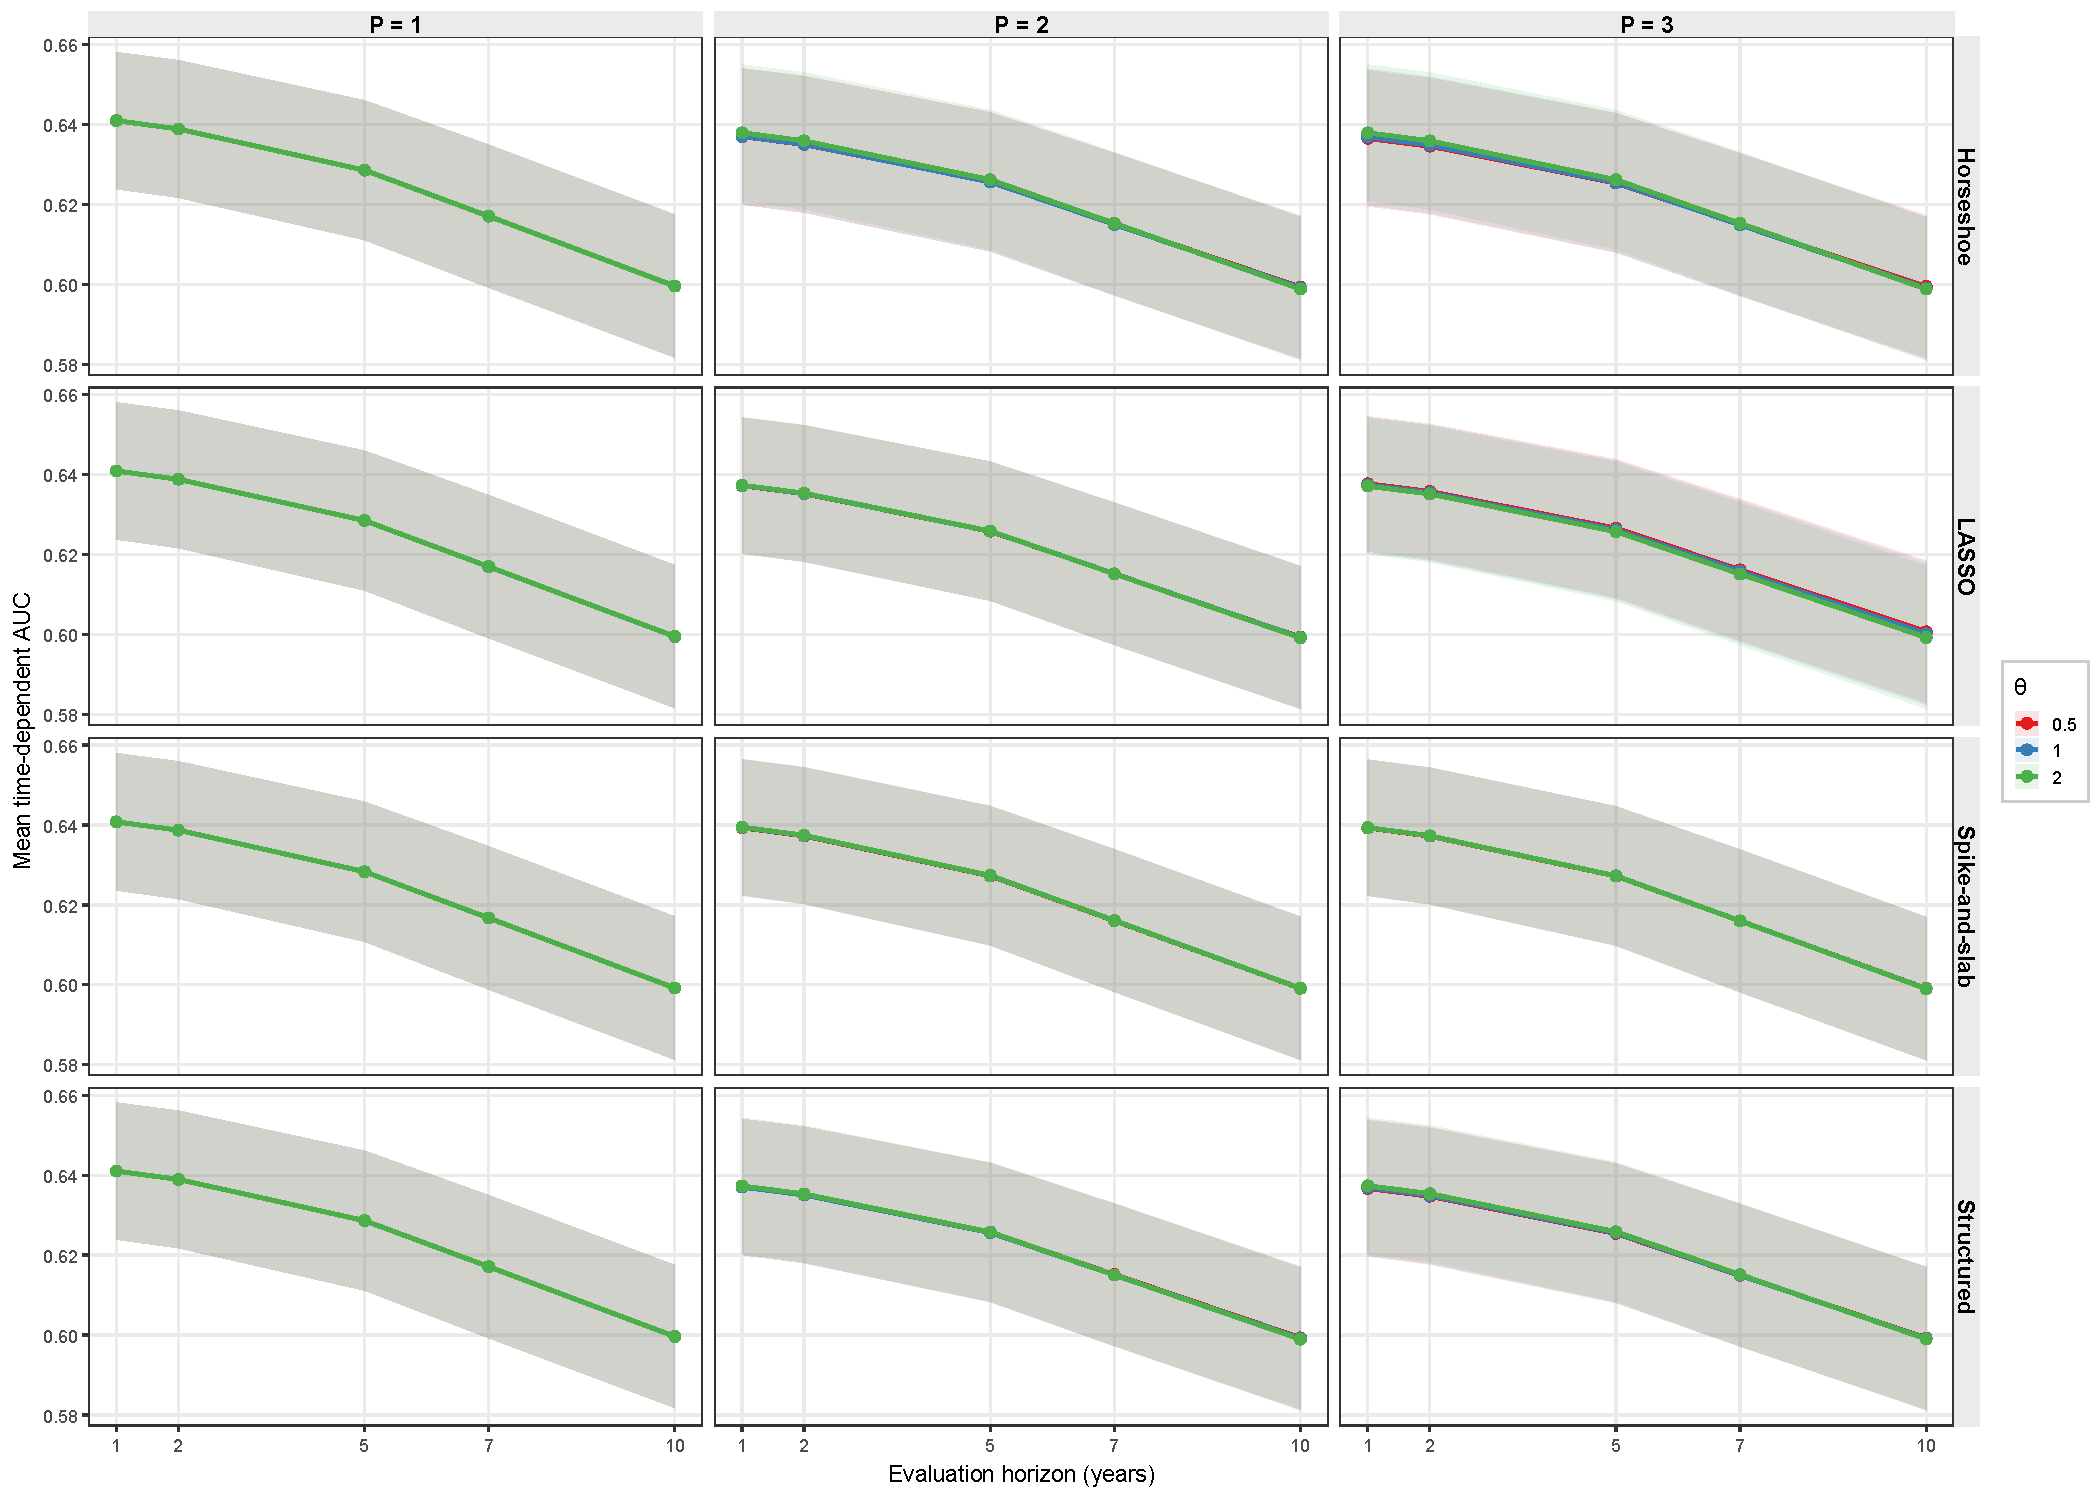
\includegraphics[width=\linewidth]{figures/fig_522_theta_sensitivity}
\caption{Sensitivity of mean tdAUC to the order penalty $\theta \in
\{0.5, 1.0, 2.0\}$, faceted by prior family and interaction order $P$.
Ribbons: $\pm1.96$\,SE.}
\label{fig:theta_sensitivity}
\end{figure}

\begin{figure}[htbp]
\centering
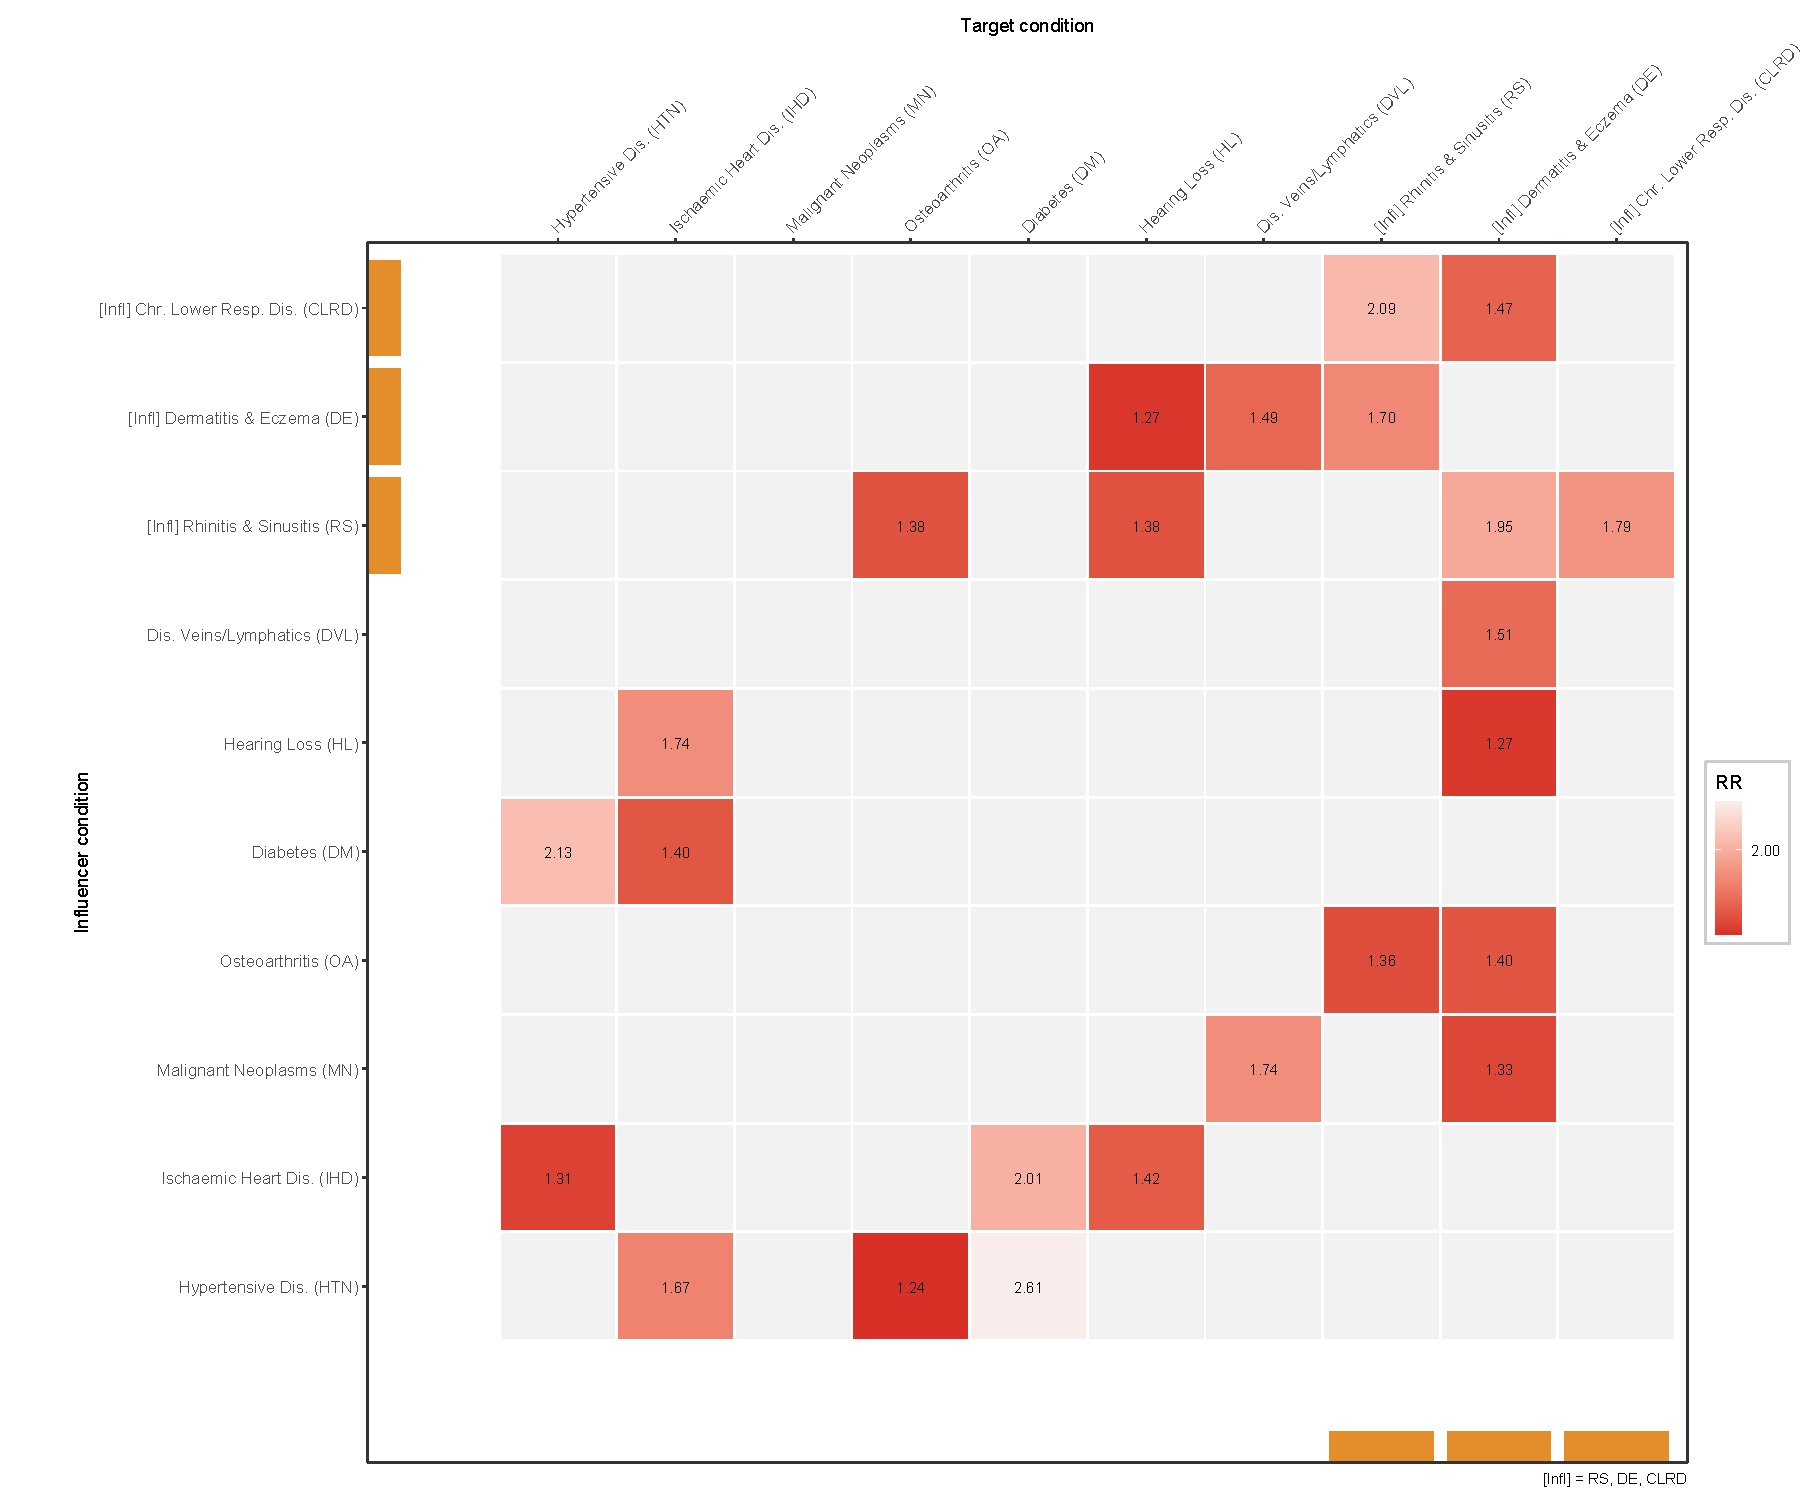
\includegraphics[width=\linewidth]{figures/fig_524b_rr_heatmap}
\caption{Posterior mean rate ratio for active edges (PIP $\geq 0.50$).
Blue = excitatory; red = inhibitory; grey = masked.  Amber bar = inflammatory
cluster.}
\label{figA:rr_network}
\end{figure}

\begin{figure}[htbp]
\centering
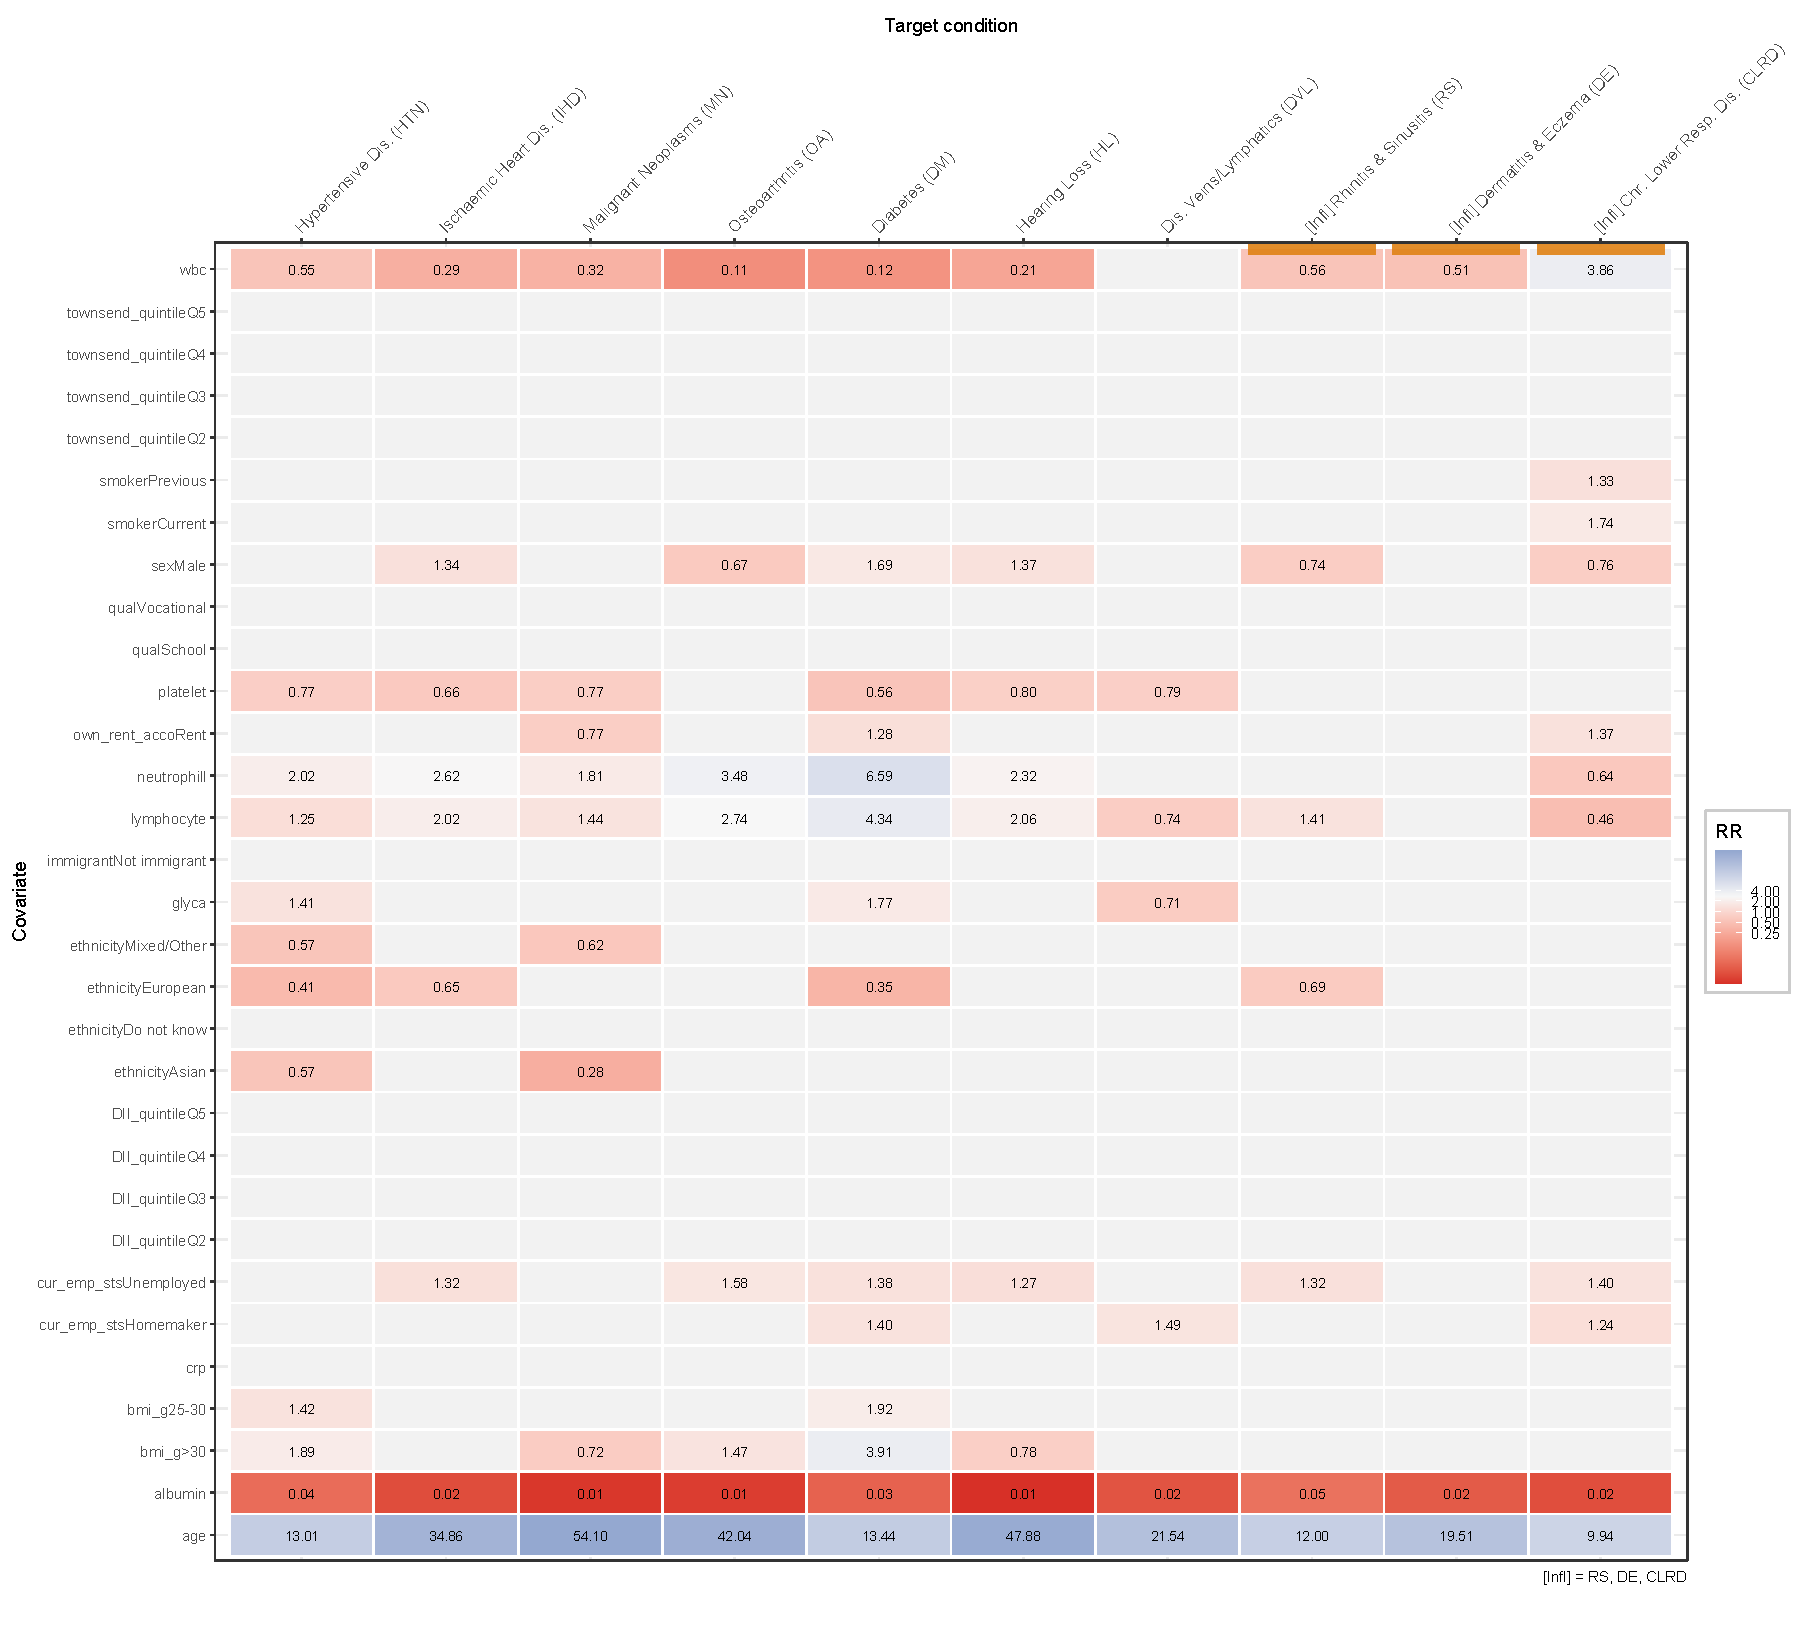
\includegraphics[width=\linewidth]{figures/fig_529b_rr_covariates}
\caption{Posterior mean rate ratio matrix for covariate--condition pairs.
Grey: PIP\,$<$\,0.50.  Amber bar = inflammatory targets.}
\label{figA:rr_covariates}
\end{figure}

\begin{figure}[htbp]
\centering
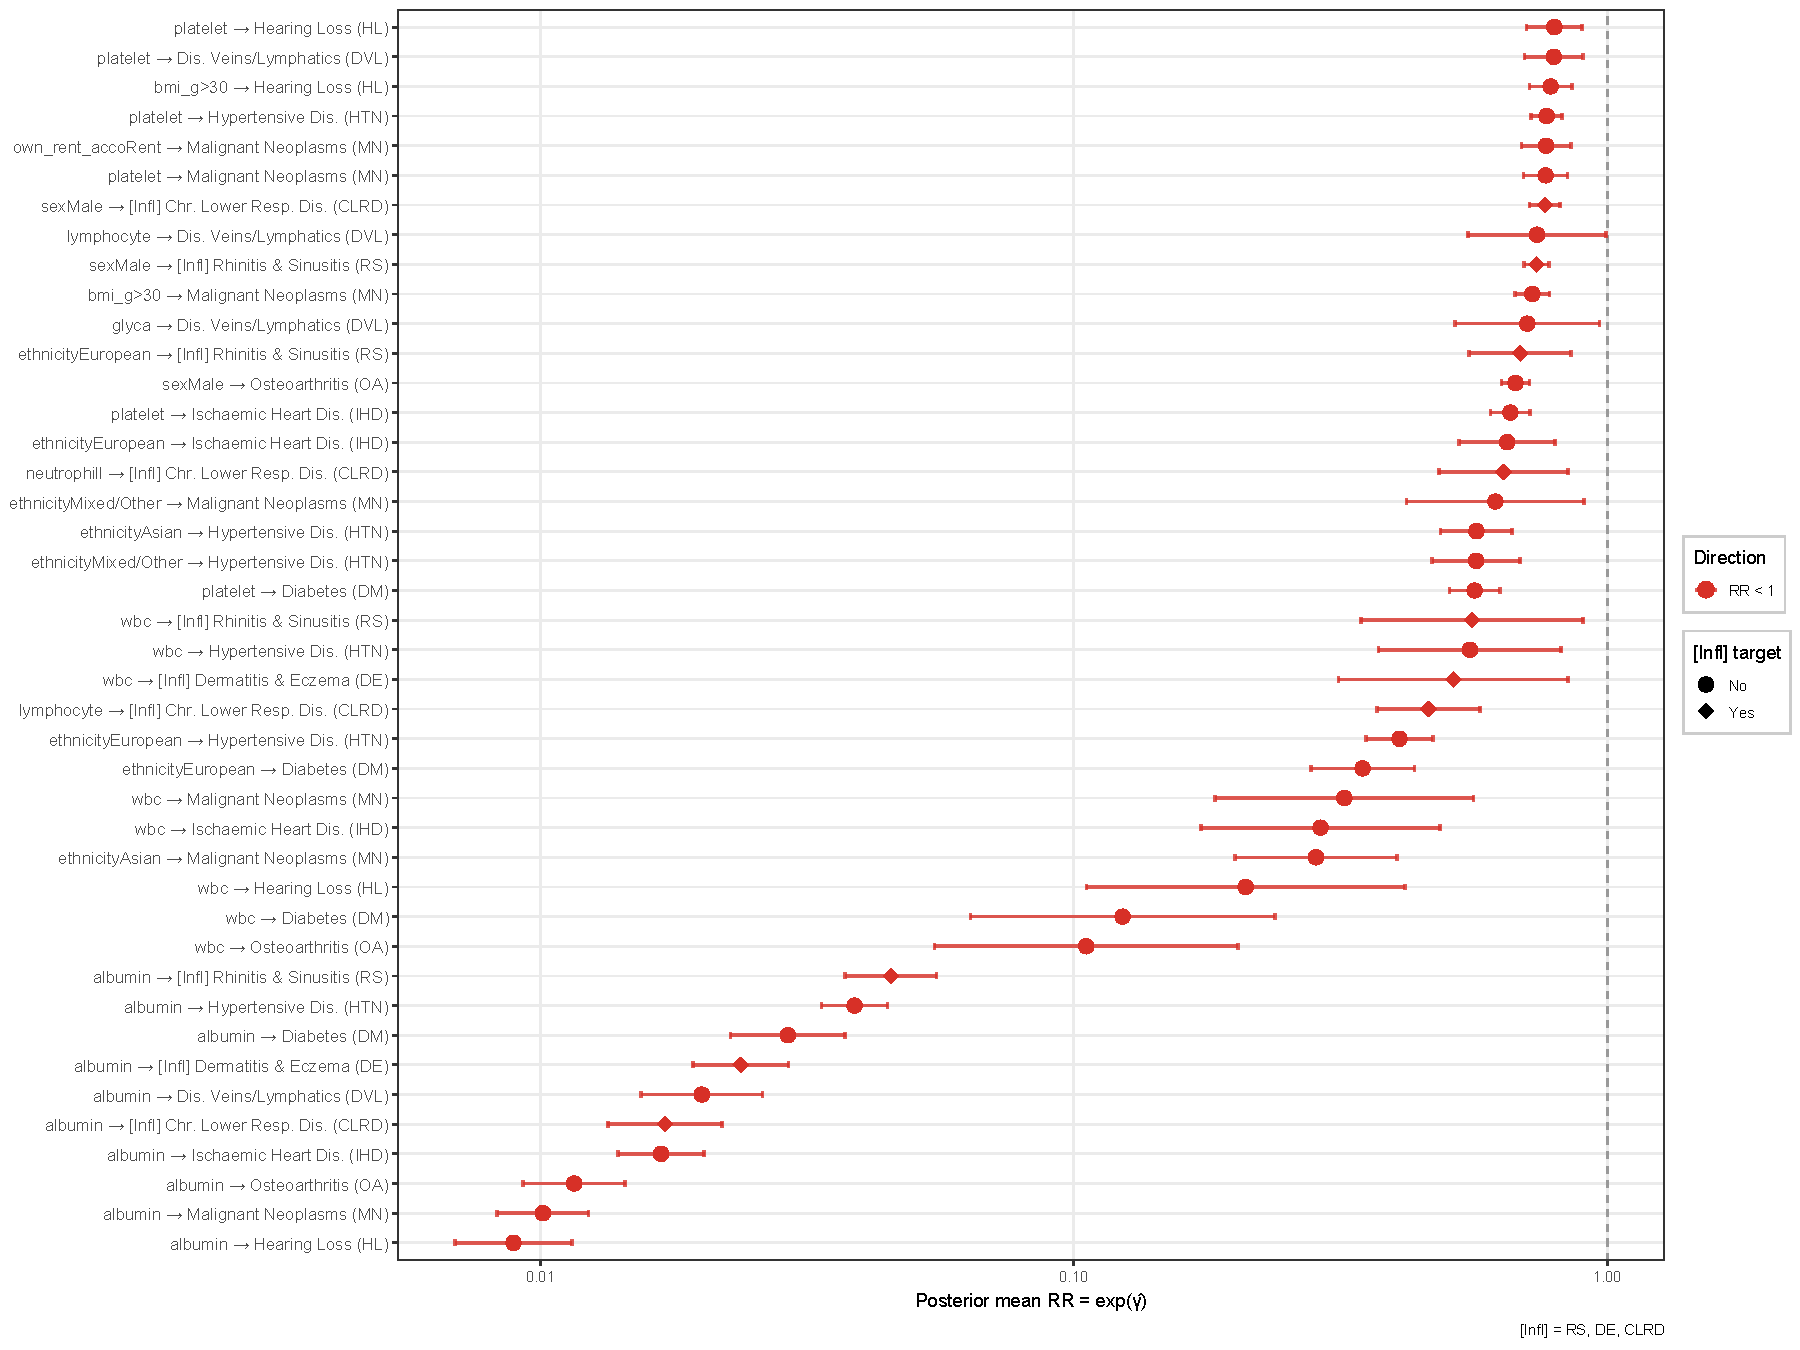
\includegraphics[width=\linewidth]{figures/fig_529d_covariate_forest}
\caption{Forest plot of posterior mean rate ratios for inhibitory covariates (RR $<1$ and PIP\,$\geq$\,0.50).  95\% credible intervals from NUTS. Spike-and-slab; $\theta=1$; $P=2$.}
\label{fig:rr_covariates_forest2}
\end{figure}




%%%%%%% Simulation supplemetary figure %%%%%%%%%%%%%%%

\begin{figure}[H]
\centering
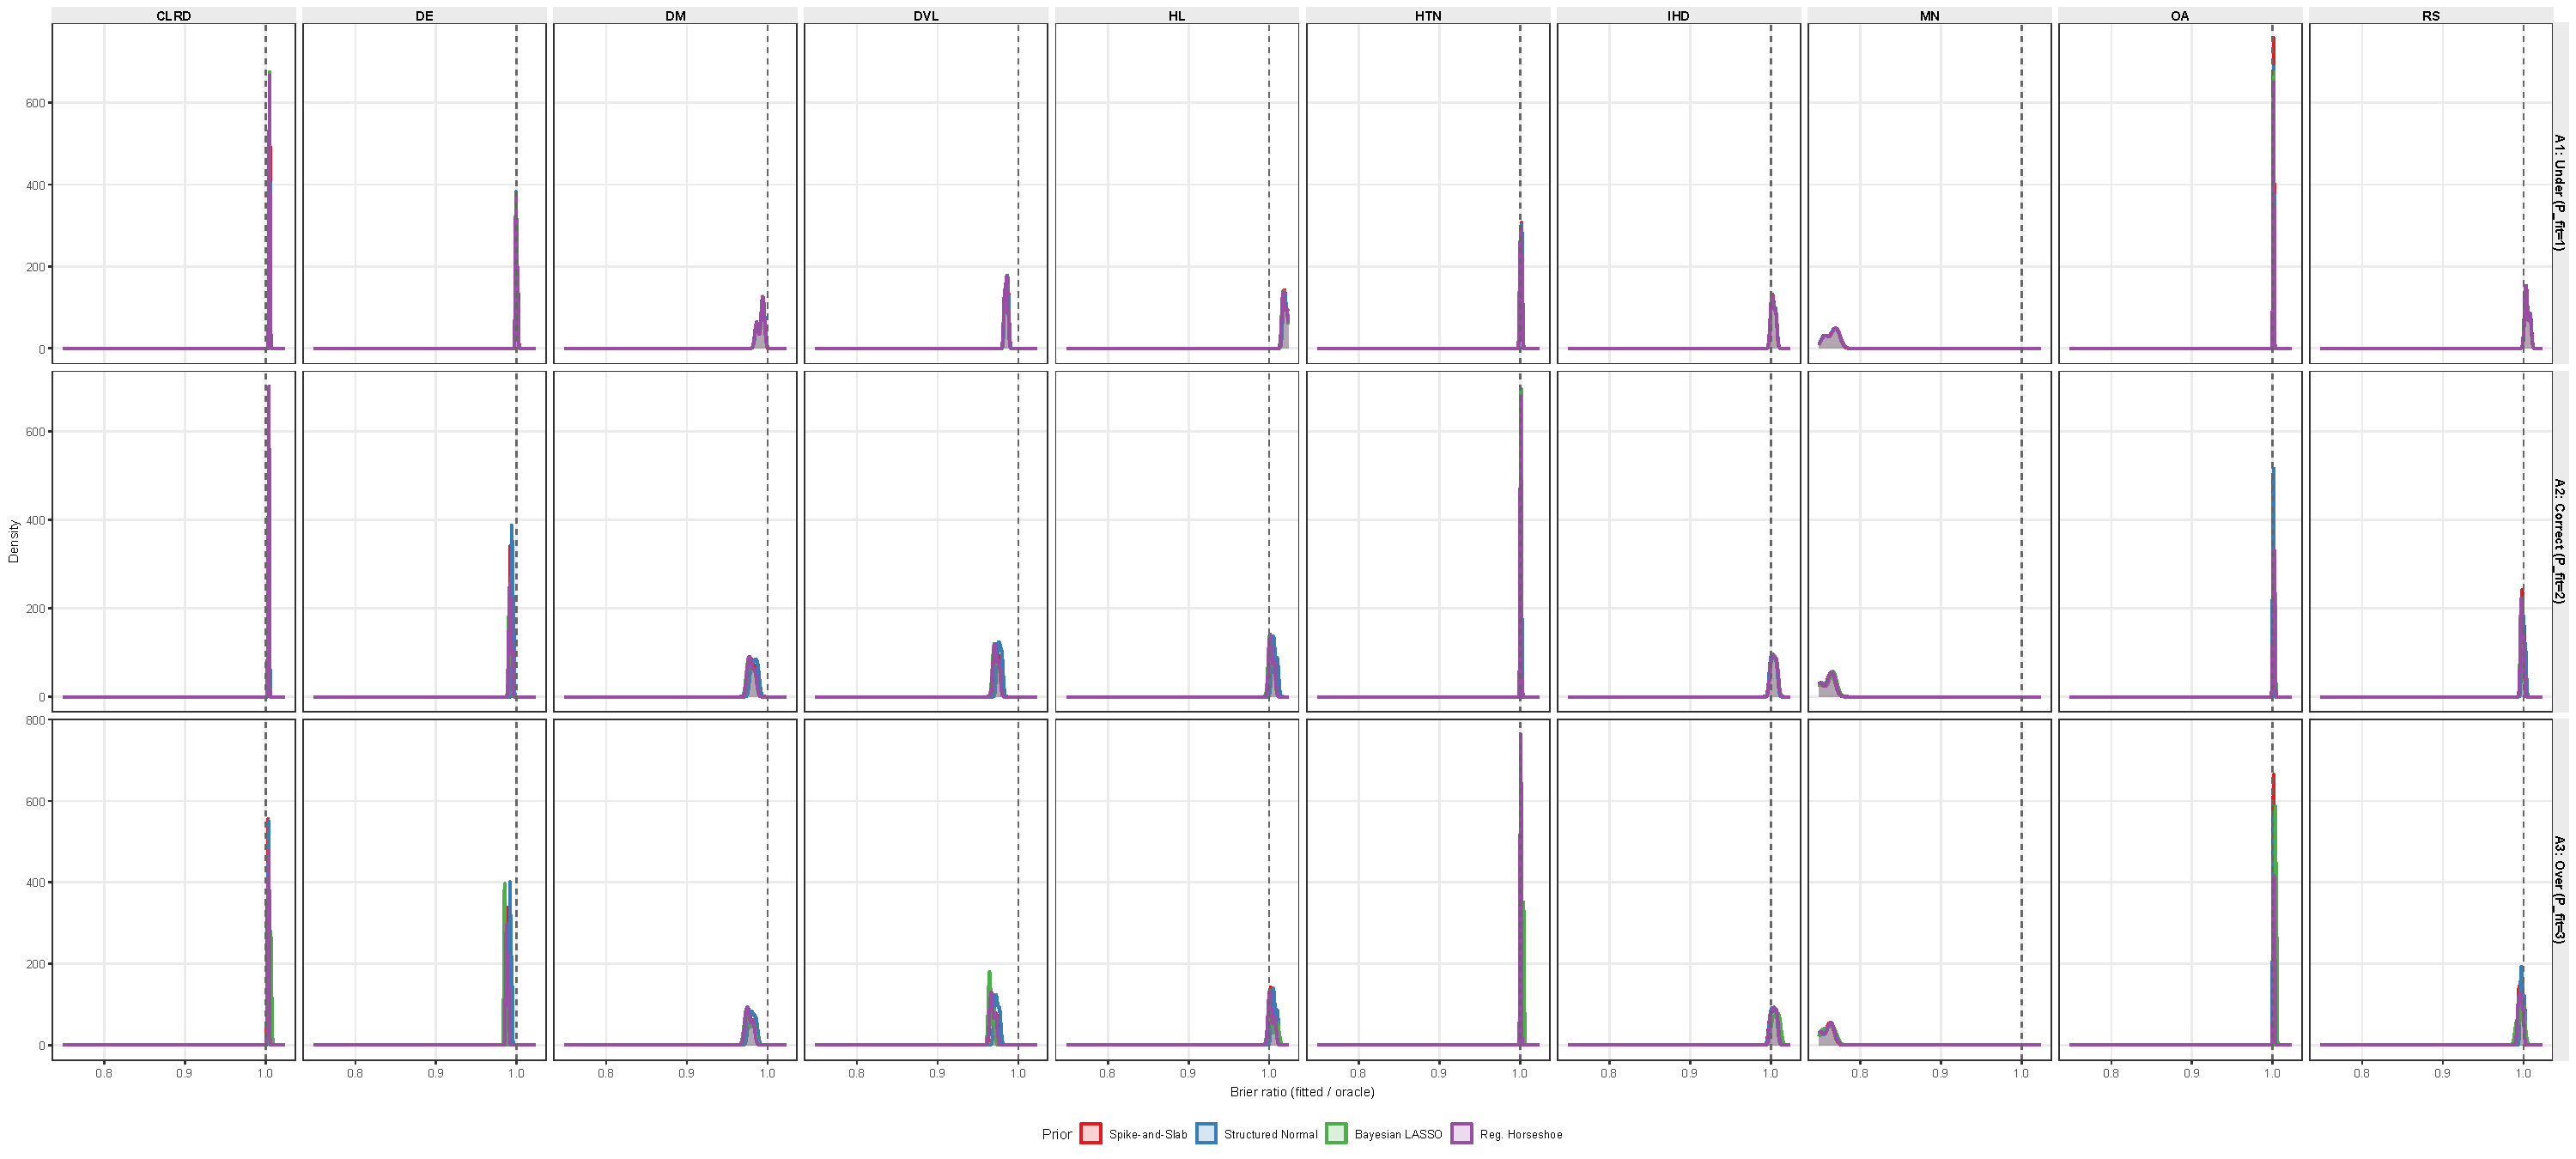
\includegraphics[width=\linewidth]{sim_results/figures/fig5d_oracle_efficiency.pdf}
\caption{Oracle efficiency (fitted Brier / oracle Brier) by analysis model,
condition, and prior.  Dashed line at 1.0; values above 1.0 indicate
efficiency loss relative to the true rate model.}
\label{fig:oracle}
\end{figure}

\end{document}
